\documentclass{amsart}

%Packages
%%%%%%%%%%%%%%%%%%%%%%%%%%%%%%%%%%%%%%%%%%%%%%%
\usepackage[alphabetic,initials,nobysame]{amsrefs}
\usepackage{amssymb,mathtools,mathrsfs,comment,todonotes,color}
\usepackage{hyperref} %cleveref has to be loaded after hyperref
\usepackage[shortlabels]{enumitem}
\usepackage{caption}
\usepackage[percent]{overpic}
\usepackage{esint} %average integral symbol

\usepackage{pgfplots}
\pgfplotsset{compat=1.13}
\usetikzlibrary{arrows}
%%%%%%%%%%%%%%%%%%%%%%%%%%%%%%%%%%%%%%%%%%%%%%%

\BibSpec{collection.article}{%
	+{}  {\PrintAuthors}				{author}
	+{,} { \textit}                     {title}
	+{.} { }                            {part}
	+{:} { \textit}                     {subtitle}
	+{,} { \PrintContributions}         {contribution}
	+{,} { \PrintConference}            {conference}
	+{}  {\PrintBook}                   {book}
	+{,} { }                            {booktitle}
	+{,} { }							{series}
	+{,} { }							{publisher}
	+{,} { }							{address}
	+{,} { \PrintDateB}                 {date}
	+{,} { pp.~}                        {pages}
	+{,} { }                            {status}
	+{,} { \PrintDOI}                   {doi}
	+{,} { available at \eprint}        {eprint}
	+{}  { \parenthesize}               {language}
	+{}  { \PrintTranslation}           {translation}
	+{;} { \PrintReprint}               {reprint}
	+{.} { }                            {note}
	+{.} {}                             {transition}
	+{}  {\SentenceSpace \PrintReviews} {review}
}

%Theorems
%%%%%%%%%%%%%%%%%%%%%%%%%%%%%%%%%%%%%%%%%%%%%%%%%%%%%%%
\theoremstyle{plain}
\newtheorem{theorem}{Theorem}
\newtheorem{lemma}[theorem]{Lemma}
\newtheorem{conjecture}{Conjecture}
\newtheorem{prop}[theorem]{Proposition}
\newtheorem{corollary}[theorem]{Corollary}
\newtheorem{fact}[theorem]{Fact}
\newtheorem{problem}[theorem]{Problem}

\theoremstyle{definition}
\newtheorem{definition}[theorem]{Definition}
\newtheorem{claim}[theorem]{Claim}

\newtheorem{innercustomthm}{Conclusion}
\newenvironment{conclusion}[1]
  {\renewcommand\theinnercustomthm{#1}\innercustomthm}
  {\endinnercustomthm}

\theoremstyle{remark}
\newtheorem{remark}[theorem]{Remark}
\newtheorem{question}[theorem]{Question}
\newtheorem{example}[theorem]{Example}
\newtheorem{note}[theorem]{Note}

\numberwithin{equation}{section}
\numberwithin{theorem}{section}
\numberwithin{conjecture}{section}
%%%%%%%%%%%%%%%%%%%%%%%%%%%%%%%%%%%%%%%%%%%%%%%%%%%%%

%Math Symbols
%%%%%%%%%%%%%%%%%%%%%%%%%%%%%%%%%%%%%%%%%%%%%%%%%%%%
\newcommand{\Conv}{\mathop{\scalebox{1.5}{\raisebox{0.0ex}{$\ast$\!}}}}%
\newcommand{\x}{\scalebox{1.2}{$\chi$} } 
\newcommand{\br}{\overline}
\newcommand{\R}{\mathbb R}
\newcommand{\T}{\mathbb T}
\newcommand{\C}{\mathbb C}
\newcommand{\D}{\mathbb D}
\newcommand{\Z}{\mathbb Z}
\newcommand{\N}{\mathbb N}
\newcommand{\Q}{\mathbb Q}
\newcommand{\p}{\mathbb P}
\newcommand{\E}{\mathbb E}
\newcommand{\1}{\mathbf 1}
\newcommand{\UHP}{\mathbb H}
\newcommand{\h}{\mathscr H}
\DeclareMathOperator{\J}{\mathcal{J}}
\DeclareMathOperator{\dist}{{\mathrm{dist}}}
\DeclareMathOperator{\diam}{{\mathrm{diam}}}
\DeclareMathOperator{\id}{{\mathrm{id}}}
\DeclareMathOperator{\inter}{{\mathrm{int}}}
\DeclareMathOperator{\re}{{\mathrm{Re}}}
\DeclareMathOperator{\im}{{\mathrm{Im}}}
\DeclareMathOperator{\length}{{\mathrm{length}}}
\DeclareMathOperator{\vol}{{\mathrm{Vol}}}
\DeclareMathOperator{\md}{\mathrm{Mod}}
\DeclareMathOperator{\cp}{\mathrm{Cap}}
\DeclareMathOperator{\area}{\mathrm{Area}}
\DeclareMathOperator{\loc}{\mathrm{loc}}
\DeclareMathOperator{\dimh}{\dim_{\mathscr H} }
\DeclareMathOperator{\proj}{\mathrm{proj}}
\DeclareMathOperator{\ver}{\mathrm{v}}
\DeclareMathOperator{\hor}{\mathrm{h}}
\DeclareMathOperator{\NED}{\mathit{NED}}
\DeclareMathOperator{\CNED}{\mathit{CNED}}
\DeclareMathOperator{\QCH}{\mathit{QCH}}
\DeclareMathOperator{\*ned}{\Conv\NED}
\DeclareMathOperator{\SH}{\mathit{SH}}
%%%%%%%%%%%%%%%%%%%%%%%%%%%%%%%%%%%%%%%%%%%%%%%%%%%%%%%%%


\begin{document}
\title{CNED sets: countably negligible for extremal distances}


\author{Dimitrios Ntalampekos}
\address{Mathematics Department, Stony Brook University, Stony Brook, NY 11794, USA.}

\thanks{The author is partially supported by NSF Grant DMS-2000096.}
\email{dimitrios.ntalampekos@stonybrook.edu}



\date{\today}
\keywords{Quasiconformal map, removable set, exceptional set, negligible set, modulus, extremal distance}
\subjclass[2020]{Primary 30C62, 30C65; Secondary 30C35, 30C75, 30C85, 31A15, 31B15, 46E35.}

\setcounter{tocdepth}{1}
%\makeatletter
%\def\l@subsection{\@tocline{2}{0pt}{2.5pc}{5pc}{}}
%\makeatother

\begin{abstract}
The author has recently introduced the class of $\CNED$ sets in Euclidean space, generalizing the classical notion of $\NED$ sets, and shown that they are quasiconformally removable. A set $E$ is $\CNED$ if the conformal modulus of a curve family is not affected when one restricts to the subfamily intersecting $E$ at countably many points. We prove that several classes of sets that were known to be removable are also $\CNED$, including sets of $\sigma$-finite Hausdorff $(n-1)$-measure and boundaries of domains with $n$-integrable quasihyperbolic distance. Thus, this work puts in common framework many known results on the problem  of quasiconformal removability and suggests that the $\CNED$ condition should also be necessary for  removability. We give a new necessary and sufficient criterion for closed sets to be (\textit{C})\textit{NED}. Applying this criterion, we show that countable unions of closed (\textit{C})\textit{NED} sets are (\textit{C})\textit{NED}. Therefore we enlarge significantly the known classes of quasiconformally removable sets. 
\end{abstract}

\maketitle

\tableofcontents

\section{Introduction}

\subsection{Definitions}

Before presenting our results, we first discuss some background. We assume throughout that $n\geq 2$. For an open set $U\subset \R^n$ and two continua  {$F_1,F_2\subset  U$} the family of curves joining $F_1$ and $F_2$ inside $U$ is denoted by $\Gamma(F_1,F_2;U)$. For a set $E\subset \R^n$ we denote by $\mathcal F_0(E)$ the family of curves in $\R^n$ that do not intersect $E$, {except possibly at the endpoints}, and by $\mathcal F_{\sigma}(E)$ the family of curves in $\R^n$ that intersect $E$  at countably many points, not counting multiplicity. 

A set $E\subset \R^n$ is \textit{negligible for extremal distances} if for every pair of non-empty, disjoint continua $F_1,F_2\subset \R^n$ we have
\begin{align*}
\md_n \Gamma(F_1,F_2;\R^n) =\md_n (\Gamma(F_1,F_2;\R^n)\cap \mathcal F_0(E)).
\end{align*}
In this case, we write $E\in \NED$; note that we suppress the dimension $n$ in this notation. If, instead, there exists a uniform constant $M\geq 1$ such that 
\begin{align*}
\md_n \Gamma(F_1,F_2;\R^n)\leq M\cdot\md_n (\Gamma(F_1,F_2;\R^n)\cap \mathcal F_0(E)),
\end{align*}
we say that $E$ is \textit{weakly} $\NED$ and we write $E\in \NED^w$. We remark that we do not require $E$ to be closed. %There is plenty of literature on closed $\NED$ sets. %Classically, one requires that the above equality holds for continua $F_1$ and $F_2$ that are disjoint from $E$. We show in Section \ref{section:ned_classical} that our definition agrees with the classical one for closed sets. 
For closed sets, the classes $\NED$ and $\NED^w$ agree \cite{AseevSycev:removable}. 

The author in \cite{Ntalampekos:metric_definition_qc} introduced the class of $\CNED$ sets, that is, \textit{countably negligible for extremal distances}. We say that a set $E\subset \R^n$ is of class $\CNED$ if
\begin{align*}
\md_n \Gamma(F_1,F_2;\R^n) =\md_n (\Gamma(F_1,F_2;\R^n)\cap \mathcal F_{\sigma}(E))
\end{align*}
for every pair of non-empty, disjoint continua $F_1,F_2\subset \R^n$. In this case we write $E\in \CNED$. As above, we also define the class $\CNED^w$ in the obvious manner. Again, $E$ need not be closed  and the dimension $n$ is suppressed in this notation. For closed sets we show in Theorem \ref{theorem:criterion_compact} that the classes $\CNED$ and $\CNED^w$ agree. The monotonicity of modulus implies that $\NED\subset \CNED \subset \CNED^w.$



\subsection{Properties of negligible sets}

Closed $\NED$ sets have been studied extensively in the plane by Ahlfors and Beurling in \cite{AhlforsBeurling:Nullsets}, where they proved that these sets coincide with the closed sets $E\subset \C$ that are \textit{removable for conformal embeddings} or else \textit{$S$-removable}; that is, every conformal embedding of $\C\setminus E$ into $\C$ is the restriction of a M\"obius transformation. See also Pesin's work \cite{Pesin:removable}. Equivalently, we may replace conformal with quasiconformal maps in this definition. See \cite{Younsi:removablesurvey} for a survey. V\"ais\"al\"a initiated the study of closed $\NED$ sets in higher dimensions \cite{Vaisala:null}, proving that closed sets of Hausdorff $(n-1)$-measure zero are of class $\NED$. The result of Ahlfors--Beurling was partially generalized in higher dimensions by Aseev--Sy\v{c}ev \cite{AseevSycev:removable} and Vodopyanov--Goldshtein \cite{VodopjanovGoldstein:removable}, who proved that if a closed set $E\subset \R^n$, $n\geq 3$, is of class $\NED$, then it is removable for quasiconformal embeddings. The converse is not known in dimensions $n\geq 3$. Finally, a characterization of closed $\NED$ sets in $\R^n$ was provided by Vodopyanov--Goldshtein \cite{VodopjanovGoldstein:removable}, who proved that closed $\NED$ sets coincide with sets that are removable for the Sobolev space $W^{1,n}$. We direct the reader to  the introduction of \cite{Aseev:nedhyperplane} for a survey of the known results. $\NED$ sets are closely related to quasiextremal distance ($\mathit{QED}$) exceptional sets, introduced by Gehring--Martio \cite{GehringMartio:QEDdomains}. As remarked, here we will work with $\NED$ sets that are not necessarily closed. 

The relation between $\CNED$ sets and quasiconformal maps was unveiled in \cite{Ntalampekos:metric_definition_qc}. We state a special case of the main theorem.

\begin{theorem}\label{theorem:removable}
Let $E\subset \R^n$ be a closed $\CNED$ set. Then every homeomorphism of $\R^n$ that is quasiconformal on $\R^n\setminus E$ is quasiconformal on $\R^n$. 
\end{theorem}

In fact, in \cite{Ntalampekos:metric_definition_qc}*{Theorem 1.2} the set $E$ is not assumed to be closed, in which case the quasiconformality of $f$ in the set $\R^n\setminus E$ has to be interpreted appropriately, using the metric definition or a variant. 


Closed sets $E$ satisfying the conclusion of Theorem \ref{theorem:removable} are called \textit{removable for quasiconformal homeomorphisms} or else \textit{$\QCH$-removable}. The difference to $S$-removable sets that we discuss above is that here we study global homeomorphisms of $\R^n$, instead of topological embeddings of $\R^n\setminus E$. Moreover, note that if a planar set is $S$-removable, then it is $\QCH$-removable. Although we have satisfactory characterizations of the former sets by Ahlfors--Beurling \cite{AhlforsBeurling:Nullsets} in dimension $2$, it is a notoriously difficult problem to characterize $\QCH$-removable sets even in dimension $2$. The current work suggests that $\CNED$ sets could provide a characterization. 

There are many open problems related to $\QCH$-removable sets, one of which is the problem of \textit{local removability} \cite{Bishop:flexiblecurves}*{Question 4}, \cite{Ntalampekos:gasket}*{Question 2}: if a closed set $E$ is $\QCH$-removable, is it true that every topological embedding of an open set $\Omega\subsetneq \R^n$ into $\R^n$ that is quasiconformal in $\Omega\setminus E$, is quasiconformal in $\Omega$? For $\CNED$ sets an affirmative answer is provided by \cite{Ntalampekos:metric_definition_qc}*{Theorem 1.2}.

Another open problem is whether the union of two $\QCH$-removable closed sets is removable \cite{JonesSmirnov:removability}. While for disjoint sets the answer is affirmative, in general, for intersecting sets this is known only in the cases of totally disconnected sets and quasicircles \cite{Younsi:RemovabilityRigidityKoebe}*{Theorem 4}. We prove here that countable unions of closed $\NED$ and $\CNED$ sets are $\NED$ and $\CNED$, respectively. 

\begin{theorem}\label{theorem:unions}
Let $E_i$, $i\in \N$, be a countable collection of closed subsets of $\R^n$.
\begin{enumerate}[\upshape(i)]\smallskip
	\item $\displaystyle{\textrm{If $E_i$ is $\NED$ for each $i\in \N$, then $\bigcup_{i\in \N} E_i$ is $\NED.$}}$\label{item:union:i}\smallskip
	\item $\displaystyle{\textrm{If $E_i$ is $\CNED$ for each $i\in \N$, then $\bigcup_{i\in \N} E_i$ is $\CNED.$}}$\label{item:union:ii}
\end{enumerate}
\end{theorem}

In the case that a countable union of closed $\NED$ sets is \textit{closed}, this result follows from the Baire category theorem \cite{Younsi:removablesurvey}*{Section 4}. The case of \textit{non-closed} unions is significantly more complicated, since they could even be dense.  The proof is given in Section \ref{section:union} and relies on an intricate characterization of $\NED$ and $\CNED$ sets from Section \ref{section:criteria}. We give a vague formulation of this characterization here. 

\begin{theorem}
A closed set $E\subset \R^n$ is $\NED$ (resp.\ $\CNED$) if and only if for every $n$-integrable metric $\rho\, ds$, almost every path $\gamma$ in $\R^n$ can be perturbed by an arbitrarily small amount of $\rho$-length to avoid the set $E$ (resp.\ to intersect the set $E$ at countably many points). 
\end{theorem}

See Theorem \ref{theorem:criterion_compact} for a precise statement. Another application of this characterization is the removability of $\CNED$ sets for continuous Sobolev functions. The proof is given in Section \ref{section:sobolev}.
\begin{theorem}\label{theorem:sobolev_intro}
Let $E\subset \R^n$ be a closed $\CNED$ set. Then every continuous function $f\colon \R^n\to \R$ with  $f\in W^{1,n}(\R^n\setminus E)$ lies in $W^{1,n}(\R^n)$. 
\end{theorem}


\subsection{Examples of negligible sets}
So far we understand some general classes of $\QCH$-removable sets. First, sets of $\sigma$-finite Hausdorff $(n-1)$-measure are removable as shown by Besicovitch  \cite{Besicovitch:Removable} in dimension $2$ and by Gehring \cite{Gehring:Rings} in higher dimensions. Thus, we can say that such sets are removable for \textit{rectifiability} reasons.

Next, it is known that sets with good geometry, such as quasicircles, are removable in dimension $2$. More generally, in all dimensions, boundaries of John domains, H\"older domains, and domains with $n$-integrable quasihyperbolic distance are removable  \cites{Jones:removability, JonesSmirnov:removability, KoskelaNieminen:quasihyperbolic}. Roughly speaking, all of these sets have either no outward cusps or  some outward cusps,  but not too many on average. Thus, these sets are removable for \textit{geometric} reasons.

Finally, $\NED$ sets are removable as well due to \cite{AhlforsBeurling:Nullsets} in dimension $2$ and   \cites{AseevSycev:removable,VodopjanovGoldstein:removable} in higher dimensions. Thus, one could say that $\NED$ sets are removable because they are small in a \textit{potential theoretic} sense. Note that all $\NED$ sets are necessarily totally disconnected in dimension $2$.

The three classes of sets are mutually singular in a sense. Namely, there are rectifiable sets that have bad geometry and are large from a potential theoretic point of view. For example, consider a rectifiable curve with a dense set of both inward and outward cusps. Likewise, there are sets with good geometry that are not rectifiable and are large for potential theory. As an example, take a quasicircle of Hausdorff dimension larger than $1$. Finally, there are sets that are small in a potential theoretic sense, but are large in terms of rectifiability and have bad geometry. For example, consider a Cantor set $E\subset \R$ of measure zero and Hausdorff dimension $1$, and then take the set $E\times E$; this is an $\NED$ set by \cite{AhlforsBeurling:Nullsets}*{Theorem 10} since its projections to the coordinate directions have measure zero. 

A natural question is whether one can reconcile these three different worlds. In other words, is there a common reason for which all of the above classes of sets are $\QCH$-removable?  We provide an affirmative answer to this question.


\begin{theorem}\label{theorem:cned}
The following sets are of class $\CNED$ in $\R^n$.
\begin{enumerate}[\upshape(i)]
	\item Sets of class $\NED$.\label{item:cned:i}
	\item Sets of $\sigma$-finite Hausdorff $(n-1)$-measure. \label{item:cned:ii}
	\item Boundaries of domains with $n$-integrable quasihyperbolic distance. \label{item:cned:iii}
\end{enumerate}
\end{theorem}

The class of sets in \ref{item:cned:iii} is defined and discussed in Section \ref{section:quasi}, where we also give the proof. This class includes quasicircles, boundaries of John domains, and boundaries of H\"older domains. As discussed earlier, \ref{item:cned:i} is immediate; however, the other conclusions are new. The technique used for the proof of \ref{item:cned:ii} allows us to generalize a result of V\"ais\"al\"a \cite{Vaisala:null}, stating that a closed set $E\subset \R^n$ with Hausdorff $(n-1)$-measure zero is of class $\NED$, to non-closed sets.

\begin{theorem}\label{theorem:zero}
Let $E\subset \R^n$ be a set of Hausdorff $(n-1)$-measure zero. Then $E$ is $\NED$.
\end{theorem}

Theorem \ref{theorem:cned} \ref{item:cned:ii} and Theorem \ref{theorem:zero} are proved in Section \ref{section:perturbation} with the aid of the notion of a \textit{family of curve perturbations}; see Theorem \ref{theorem:perturbation_hausdorff}. Roughly speaking, such curve families contain almost every parallel translate of a curve and almost every radial segment. The main theorem of that section is Theorem \ref{theorem:perturbation_family}, which asserts that the modulus of a curve family remains unaffected, if one restricts to the intersection of that family with a family of curve perturbations. 



Combining Theorems \ref{theorem:removable}, \ref{theorem:unions}, and \ref{theorem:cned}, we obtain the next removability result.

\begin{theorem}
Let $E\subset \R^n$ be a closed set that admits a decomposition into countably many sets $E_i$, $i\in \N$, each of which is contained in a closed set that is either $\NED$, or has $\sigma$-finite Hausdorff $(n-1)$-measure, or is the boundary of a domain with $n$-integrable quasihyperbolic distance. Then $E$ is $\CNED$ and $\QCH$-removable.
\end{theorem}

We also present some further examples. We show in Theorem \ref{theorem:projection} that planar sets (not necessarily closed) whose projection to each coordinate axis has measure zero are $\NED^w$, generalizing a result of Ahlfors--Beurling for closed sets \cite{AhlforsBeurling:Nullsets}*{Theorem 10}. Theorem \ref{theorem:projection} is used in the proof of Theorem \ref{example:ned} below. In Section \ref{section:nonmeasurable} we present an example of a non-measurable $\CNED$ set, constructed by Sierpi\'nski.


The results of this paper have already found an application in the problem of \textit{rigidity of circle domains}. A connected open set $\Omega$ in the Riemann sphere $\widehat{\C}$ is a \textit{circle domain} if each boundary component of $\Omega$ is either a circle or a point. A circle domain $\Omega$ is \textit{conformally rigid} if every conformal map from $\Omega$ onto another circle domain is the restriction of a M\"obius transformation of  $\widehat \C$. He--Schramm \cite{HeSchramm:Rigidity} proved that circle domains whose boundary has $\sigma$-finite Hausdorff $1$-measure are rigid. Later, Younsi and the author \cite{NtalampekosYounsi:rigidity} proved the rigidity of circle domains with $2$-integrable quasihyperbolic distance (as in Theorem \ref{theorem:cned} \ref{item:cned:iii}). It is conjectured that rigidity of a circle domain is equivalent to  $\QCH$-removability of the boundary. The next result incorporates all previous results and provides strong evidence towards this conjecture. 

\begin{theorem}[\cite{Ntalampekos:rigidity_cned}]
A circle domain is conformally rigid if every compact subset of its point boundary components is $\CNED$. 
\end{theorem}

The proof features especially Theorem \ref{theorem:unions} and the characterization of $\CNED$ sets given in Theorem \ref{theorem:criterion_compact}.

\subsection{Examples of non-negligible sets}
We remark that in Theorem \ref{theorem:unions} we are not requiring that the union of the closed sets $E_i$ be closed. However, both cases of the theorem fail without assuming that each individual set $E_i$ is closed. 

\begin{theorem}\label{example:ned}
There exist Borel $\NED$ sets $E_1,E_2 \subset \R^2$ such that $E_1\cup E_2$ is a closed set that is neither $\NED$ nor $\CNED$ nor $\QCH$-removable. 
\end{theorem}

The proof is given in Section \ref{section:nonexamples}. One can construct a more basic example with $E_1\cup E_2\notin \NED$ as follows. Tukia \cite{Tukia:hausdorff} gives an example of a set $E_1\subset [0,1]$ of full measure that can be mapped under a quasiconformal map of $\C$ onto a set of $1$-measure zero in the real line. Note that sets of $1$-measure zero are $\NED$ by Theorem \ref{theorem:zero} and such $\NED$ sets are quasiconformally invariant by Corollary \ref{corollary:qc_invariance}. Thus, $E_1$ is $\NED$. Also, $E_2=[0,1]\setminus E_1$ is $\NED$ because it has measure zero. However, $E_1\cup E_2=[0,1]$, which is not totally disconnected, so it is not $\NED$. 

Compared to $\NED$ sets, it is significantly harder to produce sets that are not $\CNED$. For the proof of Theorem \ref{example:ned} we use tools from the existing literature, and in particular from a work of Wu \cite{Wu:cantor}, to construct $\NED$ sets $E_1$ and $E_2$ such that $E_1\cup E_2$ is the product of a Cantor set in $\R$ with $[0,1]$. Such sets are not $\QCH$-removable (see \cite{Carleson:null} or the Introduction of \cite{Ntalampekos:removabilitydetour}) and thus they are not $\CNED$ by Theorem \ref{theorem:removable}; this can be proved directly in this simple situation.

As a corollary of Theorem \ref{example:ned} and \cite{Ntalampekos:metric_definition_qc}*{Theorem 1.2}, we obtain that unions of exceptional sets for the metric definition of quasiconformality are not necessarily exceptional. Here $H_f$ denotes the metric distortion of a map $f$; see \cite{Ntalampekos:metric_definition_qc}. 

\begin{corollary}
There exist Borel sets $E_1,E_2\subset \R^2$ such that $E_1\cup E_2$ is closed and for each $i\in \{1,2\}$, every homeomorphism $f$ of $\R^2$ with 
$$\sup_{x\in \R^2\setminus E_i}H_f(x)<\infty$$
is quasiconformal, but there exists a homeomorphism $g$ of $\R^2$ that is quasiconformal in $\R^2\setminus (E_1\cup E_2)$ and not quasiconformal in $\R^2$.
\end{corollary}


Finally, we end the introduction with some remarks on non-removable sets. In dimension $2$ it is known that all sets of positive area are not $\QCH$-removable \cite{KaufmanWu:removable}. There are Jordan curves of Hausdorff dimension $1$ that are non-removable \cites{Kaufman:graphnonremovable,Bishop:flexiblecurves}. Moreover, if $C\subset \R$ is a Cantor set, then $C\times [0,1]$ is non-removable as we discussed above. More interestingly, Wu \cite{Wu:cantor} proved that if $E,F\subset \R$ are Cantor sets and $E\notin \NED$, then $E\times F$ is non-removable; the converse is not true since $\NED$ sets can have positive length \cite{AhlforsBeurling:Nullsets}. More recently, the current author studied the problem of removability for fractals with infinitely many complementary components and proved that the Sierpi\'nski gasket and all Sierpi\'nski carpets are non-removable \cites{Ntalampekos:gasket,Ntalampekos:CarpetsNonremovable}. The latter result was generalized to higher dimensional carpets, known as Sierpi\'nski spaces, by the author and Wu \cite{NtalampekosWu:Sierpinski}. 

Gaskets and carpets fall into the general class of \textit{residual sets of packings}. A packing $\mathcal P$ in $\R^n$ is a collection of bounded, connected open sets $D_i$, $i\in \N\cup \{0\}$, such that $D_i\subset D_0$ for every $i\in \N$ and $D_i\cap D_j=\emptyset$ for $i,j\in \N$ with $i\neq j$.  The residual set of the packing $\mathcal P$ is the set 
\begin{align*}
\br {D_0} \setminus \bigcup_{i\in \N}D_i.
\end{align*}
We observe below that in many cases such residual sets  are not $\CNED$. 

\begin{prop}\label{proposition:packings}
Let $\mathcal P=\{D_i\}_{i\in \N\cup \{0\}}$ be a packing in $\R^n$ such that $\partial D_i\cap \partial D_j$ is  countable for $i\neq j$, $i,j\in \N\cup\{0\}$. Then the residual set of $\mathcal P$ is not  $\CNED$. 
\end{prop}

It was earlier observed that such residual sets in the plane can have Hausdorff dimension $1$ but not $\sigma$-finite Hausdorff $1$-measure \cite{MaioNtalampekos:packings}. Proposition \ref{proposition:packings} covers the Sierpi\'nski gasket and all Sierpi\'nski carpets. 

\subsection{Open problems}
Based on the results of this work, it is natural to propose the following problem, whose resolution would answer many of the open questions related to removable sets.

\begin{problem}\label{problem}
Do $\QCH$-removable sets coincide with closed $\CNED$ sets?
\end{problem}
We also formulate a series of questions for $\CNED$ sets.

\begin{question}\label{question:positive}
If $E\subset \R^n$ is a closed set that is not $\CNED$, does there exist a homeomorphism of $\R^n$ that is quasiconformal in $\R^n\setminus E$ and maps $E$ to a set of positive $n$-measure?
\end{question}
A positive answer to this question would resolve Problem \ref{problem} and thus it would also resolve among others the problems of local removability and of removability of unions of removable sets mentioned earlier. For closed $\NED$ sets in the plane the answer to the corresponding question is already known to be affirmative by Ahlfors--Beurling \cite{AhlforsBeurling:Nullsets}: if $E\notin \NED$, then there exists a conformal embedding $f\colon \R^2\setminus E \to \R^2$ such that the complement of $f(\R^2\setminus E)$ has positive area.
\begin{question}If $E\subset \R^n$ is a closed set that is not $\CNED$, does there exist a totally disconnected closed subset of $E$ that is not $\CNED$?
\end{question}
If yes, it would suffice to answer Question \ref{question:positive} for totally disconnected sets, which could be more approachable. Note that $\NED$ sets in the plane are already totally disconnected, so this makes the study of these sets more accessible.


\begin{problem}
Do removable sets for continuous $W^{1,n}$ functions  coincide with closed $\CNED$ sets?
\end{problem}
This problem is motivated by Theorem \ref{theorem:sobolev_intro}.  Obviously, the answer would be positive if the answer to Problem \ref{problem} were positive, in which case, $\QCH$-removable sets would coincide with removable sets for continuous $W^{1,n}$ functions. This is another open problem discussed in \cites{Bishop:flexiblecurves,JonesSmirnov:removability}. 


\subsection*{Acknowledgements}
The author would like to thank Hrant Hakobyan and Malik Younsi for their comments. 



\section{Preliminaries}\label{section:preliminaries}

\subsection{Notation and definitions}
We denote the Euclidean distance between points $x,y\in \R^n$ by $|x-y|$. For $x\in \R^n$ and $0\leq r<R$ we denote by $B(x,R)$ the open ball $\{y\in \R^n: |x-y|<R\}$ and by $A(x;r,R)$ the open ring $\{y\in \R^n: r<|x-y|<R\}$. The corresponding closed ball and ring are denoted by $\br B(x,r)$ and $\br A(x;r,R)$, respectively. If $B$ is an open (resp.\ closed) ball, then for $\lambda>0$ we denote by $\lambda B$ the open (resp.\ closed) ball with the same center as $B$ and radius multiplied by $\lambda$. We also set $S^{n-1}(x,r)=\partial B(x,r)$.  The open $\varepsilon$-neighborhood of a set $E\subset \R^n$ is denoted by $N_{\varepsilon}(E)$.

We use the notation $m_n$ for the $n$-dimensional Lebesgue measure in $\R^n$, $m_n^*$ for the outer $n$-dimensional Lebesgue measure, and $\int_{\R^n}\rho(x) \, dx$ or simply $\int \rho$ for the Lebesgue integral of a Lebesgue measurable extended function $\rho\colon \R^n\to [-\infty,\infty]$, if it exists. For such a function $\rho$, if $B$ is a measurable set with $m_n(B)\in (0,\infty)$, we define
$$\fint_B \rho= \frac{1}{m_n(B)} \int_B \rho.$$
For simplicity, extended functions will be called functions. A non-negative function is assumed to take values in $[0,\infty]$.


The cardinality of a set $E$ is denoted by $\#E$. For quantities $A$ and $B$ we write $A\lesssim B$ if there exists a constant $c>0$ such that $A\leq cB$. If the constant $c$ depends on another quantity $H$ that we wish to emphasize, then we write instead $A\leq c(H)B$ or $A\lesssim_H B$. Moreover, we use the notation $A\simeq B$ if $A\lesssim B$ and $B\lesssim A$. As previously, we write $A\simeq_H B$ to emphasize the dependence of the implicit constants on the quantity $H$. All constants in the statements are assumed to be positive even if this is not stated explicitly and the same letter may be used in different statements to denote a different constant.  

For $s\geq 0$ the \textit{$s$-dimensional Hausdorff measure} $\mathscr H^s(E)$ of a set $E\subset \R^n$ is defined by
$$\mathscr{H}^{s}(E)=\lim_{\delta \to 0} \mathscr{H}_\delta^{s}(E)=\sup_{\delta>0} \mathscr{H}_\delta^{s}(E),$$
where
$$
\mathscr{H}_\delta^{s}(E)=\inf \bigg\{ c(s)\sum_{j=1}^\infty \operatorname{diam}(U_j)^{s}: E \subset \bigcup_j U_j,\, \operatorname{diam}(U_j)<\delta \bigg\}
$$
for a normalizing constant $c(s)>0$ so that the $n$-dimensional Hausdorff measure agrees with Lebesgue measure in $\R^n$. Note that $c(1)=1$. The quantity $\mathscr{H}_\delta^{s}(E)$, $\delta\in (0,\infty]$, is called the \textit{$s$-dimensional Hausdorff $\delta$-content} of $E$. If $\delta=\infty$ we simply call this quantity the \textit{$s$-dimensional Hausdorff  content} of $E$. A standard fact that we will use is that 
\begin{align*}
\textrm{$\h^s(E)=0$ if and only if $\h^s_{\infty}(E)=0$. }
\end{align*}
We note that if $E\subset \R^n$ is a connected set, then (see 	\cite{BuragoBuragoIvanov:metric}*{Lemma 2.6.1, p.~53})
\begin{align*}
\h^1(E) \geq \h^1_{\infty}(E)=\diam(E).
\end{align*}

\begin{lemma}[\cite{Bojarski:inequality}]\label{lemma:bojarski}
Let $p\geq 1$ and $\lambda >0$. Suppose that $\{B_i\}_{i\in \N}$ is a collection of balls in $\R^n$ and $a_i$, $i\in \N$, is a sequence of non-negative numbers. Then
\begin{align*}
\left \|  \sum_{i\in \N} a_i \x_{\lambda B_i} \right \|_{L^p(\R^n)} \leq c({n,p,\lambda})  \left \|  \sum_{i\in \N} a_i \x_{B_i} \right \|_{L^p(\R^n)}.
\end{align*} 
\end{lemma}



\subsection{Rectifiable paths}
A \textit{path} or \textit{curve} is a continuous function $\gamma\colon I \to \R^n$, where $I\subset \R$ is a compact interval. The \textit{trace} of a path $\gamma$ is the image $\gamma(I)$ and will be denoted by $|\gamma|$. The \textit{endpoints} of a path $\gamma\colon [a,b]\to \R^n$ are the points $\gamma(a),\gamma(b)$ and we set $\partial \gamma= \{\gamma(a),\gamma(b)\}$. We say that a path $\widetilde \gamma$ is a \textit{weak subpath} of a path $\gamma$ if ${\#}\widetilde {\gamma}^{-1}(x)\leq \#\gamma^{-1}(x)$ for every $x\in \R^n$. In particular, this implies that $|\widetilde \gamma|\subset |\gamma|$. A path $\widetilde \gamma$ is a \textit{(strong) subpath} of a path $\gamma \colon I\to \R^n$ if $\widetilde \gamma$ is the restriction of $\gamma$ to a closed subinterval of $I$. Note that a strong subpath is always a weak subpath, but not vice versa. A path $\gamma$ is \textit{simple} if it is injective. Equivalently, $\#\gamma^{-1}(x)=1$ for each $x\in |\gamma|$. It is well-known that every path has a simple weak subpath with the same endpoints \cite{Willard:topology}*{Theorem 31.2, p.~219}. 

If $\gamma$ is a path and $E\subset \R^n$ is a set, then we say that $\gamma$ \textit{avoids} the set $E$ if $E\cap |\gamma|=\emptyset$ and intersects $E$ at (e.g.) finitely many points if $E\cap |\gamma|$ is a finite set; note that we are not taking into account the multiplicity in the latter case.

If $\gamma_i\colon [a_i,b_i]\to \R^n$, $i=1,2$, are paths such that $\gamma_1(b_1)=\gamma_2(a_2)$, then we can define the \textit{concatenation} of the two paths to be the path $\gamma\colon [a_1,b_2]\to \R^n$ such that $\gamma|_{[a_1,b_1]}=\gamma_1$ and $\gamma|_{[a_2,b_2]}=\gamma_2$. If $x,y\in \R^n$, then we denote the line segment from $x$ to $y$ by $[x,y]$. 

The \textit{length} of a path $\gamma$ is the total variation of the function $\gamma$ and is denoted by $\ell(\gamma)$. A path is \textit{rectifiable} if it has finite length. Let $\gamma\colon [a,b]\to \R^n$ be a path and $s\colon [c,d]\to [a,b]$ be an increasing or decreasing continuous surjection. Then the path $\gamma\circ s\colon [c,d]\to \R^n$ is called a  \textit{reparametrization} of $\gamma$ (by the function $s$). Every rectifiable path $\gamma$ admits a unique reparametrization $\widetilde \gamma \colon [0,\ell(\gamma)]\to \R^n$ by an increasing function so that $\ell(\widetilde \gamma|_{[0,t]})=t$ for all $t\in [0,\ell(\gamma)]$. The path $\widetilde \gamma$ is called the \textit{arclength parametrization} of $\gamma$.

If $\rho\colon \R^n \to [0,\infty]$ is a Borel function and $\gamma$ is a rectifiable path, then one can define the line integral $\int_{\gamma} \rho\, ds$ using the arclength parametrization of $\gamma$; see \cite{Vaisala:quasiconformal}*{Chapter 1, pp.~8--9}. Namely, if $\gamma\colon [0,\ell(\gamma)]\to \R^n$ is parametrized by arclength, then 
$$\int_{\gamma}\rho\, ds = \int_0^{\ell(\gamma)}\rho(\gamma(t))\, dt. $$
We gather some properties of line integrals below.

\begin{lemma}\label{lemma:paths}
Let $\gamma$ be a rectifiable path, $\widetilde \gamma$ be a weak subpath of $\gamma$, and $\rho\colon \R^n \to [0,\infty]$ be a Borel function. The following statements are true.
\begin{enumerate}[\upshape(i)]\smallskip
	\item\label{lemma:paths:i} $\displaystyle{\int_{\gamma}\rho\, ds}=  \int_{\R^n} \rho(x) \#\gamma^{-1}(x)\, d\h^1(x)$.\smallskip
	\item\label{lemma:paths:iv}$\displaystyle{\int_{|\gamma|} \rho\, d\h^1 \leq \int_{\gamma}\rho\, ds}$ with equality if $\gamma$ is simple.\smallskip
	\item\label{lemma:paths:ii} $\displaystyle{\int_{\widetilde \gamma}\rho\, ds\leq \int_{\gamma}\rho\, ds}$.\smallskip
	\item\label{lemma:paths:iii} If $G\subset \R^n$ is a Borel set such that $\h^1(G\cap |\gamma|)=0$, then 
	\begin{align*}
\int_{\gamma} \rho \, ds =  \int_{\gamma}\rho \x_{\R^n\setminus G}\, ds.
	\end{align*}
\end{enumerate}
In particular, the above statements hold for $\rho=1$, in which case $\displaystyle{\displaystyle{\int_{\gamma}\rho\, ds}=\ell(\gamma)}$.
\end{lemma}

\begin{proof}
Part \ref{lemma:paths:i} follows from \cite{Federer:gmt}*{Theorem 2.10.13, p.~177}. The inequality and equality in \ref{lemma:paths:iv} follow from \ref{lemma:paths:i}. Since $\widetilde \gamma$ is a weak subpath of $\gamma$, we have ${\#}\widetilde {\gamma}^{-1}(x)\leq \#\gamma^{-1}(x)$. Thus \ref{lemma:paths:i} implies \ref{lemma:paths:ii}. Part \ref{lemma:paths:iii} also follows from \ref{lemma:paths:i}  upon observing that $\x_{\R^n\setminus G}(x)\#\gamma^{-1}(x)= \#\gamma^{-1}(x)$ for $x\notin G\cap |\gamma|$ and thus for $\h^1$-a.e.\ $x\in \R^n$.  
\end{proof}



\subsection{Modulus}
Let $\Gamma$ be a family of curves in $\R^n$. A Borel function $\rho\colon \R^n \to [0,\infty]$ is \textit{admissible} for the path family $\Gamma$ if $$\int_{\gamma}\rho\, ds\geq 1$$
for all rectifiable paths $\gamma\in \Gamma$. For $p\geq 1$ we define the \textit{$p$-modulus} of $\Gamma$ as 
$$\md_p \Gamma = \inf_\rho \int \rho^p,$$
where the infimum is taken over all admissible functions $\rho$ for $\Gamma$. By convention, $\md_p \Gamma = \infty$ if there are no admissible functions for $\Gamma$. Note that unrectifiable paths do not affect modulus. Hence, we will assume that families of $p$-modulus zero appearing in the next considerations contain all unrectifiable paths. We will use the following standard facts about modulus:
\begin{enumerate}[label=(M\arabic*)]
\item The modulus $\md_p$ is an outer measure in the space of all curves in $\R^n$. In particular, it obeys the monotonicity and countable subadditivity laws. \label{m:outer_measure}

\item If every path of a family $\Gamma_1$ has a subpath lying in a family $\Gamma_2$, then $\md_p\Gamma_1\leq \md_p\Gamma_2.$\label{m:subordinate}

\item If $\Gamma_0$ is a path family with $\md_p\Gamma_0=0$, then the family of paths $\gamma$ that have a weak subpath in $\Gamma_0$ also has $n$-modulus zero (by Lemma \ref{lemma:paths} \ref{lemma:paths:ii}). Moreover, the family of paths that have a reparametrization contained in $\Gamma_0$ also has $p$-modulus zero. \label{m:subpath}

%\item If $\Omega\subset \R^n$ is an open set and $\rho\colon \Omega\to [0,\infty]$ is a Borel function with $\rho\in L^n_{\loc}(\Omega)$, then there exists a path family $\Gamma_0$  with $\md_n\Gamma_0=0$ such that for each path $\gamma\notin \Gamma_0$ with trace in $\Omega$ we have $\int_{\gamma}\rho\, ds<\infty$; here we implicitly assume that if $\gamma\notin \Gamma_0$, then $\gamma$ is rectifiable.\label{m:integrable}

\item If $\rho\colon \R^n\to [0,\infty]$ is a Borel function with $\rho=0$ a.e., then for the family $\Gamma_0$ of paths $\gamma$ with $\int_{\gamma}\rho\, ds>0$ we have  $\md_n\Gamma_0=0$. \label{m:zero_ae}

\item  The modulus $\md_p$ obeys the \textit{serial} law: if $\Gamma_i$, $i\in \N$, are curve families supported in disjoint Borel sets, then
\begin{align*}
\md_p\left(\bigcup_{i=1}^\infty \Gamma_i \right) \geq \sum_{i=1}^\infty \md_p \Gamma_i.
\end{align*}\label{m:serial}



%\item Suppose that $\md_p\Gamma=0$. Then the family of rectifiable curves that have a  weak subpath contained in $\Gamma$ has $p$-modulus zero (by Lemma \ref{lemma:paths} \ref{lemma:paths:ii}). Moreover, the family of curves that have a reparametrization contained in $\Gamma$ also has $p$-modulus zero. 

\item Let $E\subset \R^n$ be a set with $m_n(E)=0$. Let $\Gamma_0$ be the family of paths $\gamma$ such that $\h^1( |\gamma|\cap E)>0$. Then $\md_p\Gamma_0=0$. \label{m:positive_length}

\item For $p=n$ the modulus $\md_n$ is invariant under conformal maps.

\item Let $\Gamma=\Gamma(A(x;r,R))$ be the family of curves in $\R^n$ joining the boundary components of the ring $A(x;r,R)$.  Then 
$$\md_n\Gamma= \omega_{n-1}\left(\log\frac{R}{r} \right)^{1-n}.$$\label{m:ring}
\end{enumerate}
Here $\omega_{n-1}$ is the area of the unit sphere in $\R^n$. See \cite{Vaisala:quasiconformal}*{Chapter 1} and \cite{HeinonenKoskelaShanmugalingamTyson:Sobolev}*{Sections 5.2--5.3} for more details about modulus and proofs of these facts. 


For a path $\gamma\colon I\to \R^n$ and $x\in \R^n$ we define $\gamma+x$ to be the path $I\ni t\mapsto \gamma(t)+x$.  

\begin{lemma}\label{modulus:avoid}
Let $\Gamma$ be a family of paths in $\R^n$ with $\md_p\Gamma=0$.
\begin{enumerate}[\upshape(i)]
	\item For each rectifiable path $\gamma$ and for a.e.\ $x\in \R^n$ we have $\gamma+x\notin \Gamma$.
	\item For each line segment $L$ parallel to a direction $v\in \R^n$ and for $\h^{n-1}$-a.e.\ $x\in \{v\}^{\perp}$ we have $L+x\notin \Gamma$.
	\item For each $x\in \R^n$ and $w\in S^{n-1}(0,1)$ define $\gamma_w(t)=x+tw$, $t\geq 0$. Then for $0<r<R$ we have $\gamma_w|_{[r,R]}\notin \Gamma$ for $\h^{n-1}$-a.e.\ $w\in S^{n-1}(0,1)$.  
\end{enumerate}  
\end{lemma}
\begin{proof}
For each $\varepsilon>0$ there exists a function $\rho$ that is admissible  for $\Gamma$ with $\int \rho^p<\varepsilon$. 

For (i), let $\gamma$ be a rectifiable path in $\R^n$, parametrized by arclength. Let $r>0$ and $G_r$ be the set of $x\in B(0,r)$ such that $\gamma+x\in \Gamma$. We also fix $R>0$ such that $|\gamma+x|\subset B(0,R)$ whenever $x\in B(0,r)$. Then by Chebychev's inequality and Fubini's theorem we have
\begin{align*}
m_n^*(G_r) &\leq m_n \left(\left\{x \in B(0,r): \int_{\gamma+x} \rho\, ds \geq 1  \right\} \right) \leq \int_{B(0,r)} \int_0^{\ell(\gamma)} \rho(\gamma(t)+x)\, dtdx\\
&= \int_0^{\ell(\gamma)} \int_{B(0,r)} \rho(\gamma(t)+x)\, dxdt\leq \ell(\gamma)\|\rho\|_{L^1(B(0,R))}.
\end{align*}
As $\varepsilon\to 0$, we have $\|\rho\|_{L^p(B(0,R))} \to 0$, so $\|\rho\|_{L^1(B(0,R))}\to 0$. This shows that $m_n(G_r)=0$ for all $r>0$. Thus, $\gamma+x\notin \Gamma$ for a.e.\ $x\in \R^n$.

For part (ii), let $G_r$ be the set of $x\in B(0,r)\cap \{v\}^{\perp}$ such that $L+x\in \Gamma$. Then
\begin{align*}
\h^{n-1}(G_r) \leq \h^{n-1} \left( \left\{ x\in B(0,r)\cap \{v\}^{\perp} : \int_{L+x} \rho\, ds \geq 1  \right\}\right)\leq \|\rho\|_{L^1(D)},
\end{align*}
where $D$ is the cylinder of radius $r$ with axis $L$. We now let $\varepsilon\to 0$ as above.  

Finally, for (iii), let $G$ be the set of $w\in S^{n-1}(0,1)$ such that $\gamma_w|_{[r,R]}\in \Gamma$. Then, using polar integration we have
\begin{align*}
\h^{n-1}(G) &\leq \h^{n-1} \left( \left\{ w\in S^{n-1}(0,1) : \int_{\gamma_w|_{[r,R]}} \rho\, ds \geq 1  \right\}\right)\\
&\leq \int_{S^{n-1}(0,1)} \int_{r}^R \rho( x+tw)\, dt d\h^{n-1}(w)\lesssim_n r^{-n+1} \|\rho\|_{L^1(B(x,R))}.
\end{align*}
As before, we let $\varepsilon\to 0$ to obtain the conclusion. 
\end{proof}



\subsection{\texorpdfstring{Elementary properties of $\NED$ and $\CNED$ sets}{Elementary properties of NED and CNED sets}}\label{section:elementary}


We first recall the definitions. For an open set $U\subset \R^n$ and for any two closed sets {$F_1,F_2\subset \R^n$} the family of curves joining $F_1$ and $F_2$ inside $U$ is denoted by $\Gamma(F_1,F_2;U)$. In other words, this family contains the curves $\gamma\colon [a,b]\to \br U$ with $\gamma(a)\in F_1$, $\gamma(b)\in F_2$, and $\gamma((a,b))\subset U$.  For a set $E\subset \R^n$ we denote by $\mathcal F_0(E)$ the family of curves in $\R^n$ that do not intersect $E$, {except possibly at the endpoints}; that is, $\mathcal F_0(E)$ contains the curves $\gamma\colon [a,b]\to \R^n$ such that $|\gamma|\setminus \gamma(\{a,b\})$ does not intersect $E$. Moreover, we define $\mathcal F_{\sigma}(E)$ to be the family of curves in $\R^n$ that intersect $E$ in countably many points; that is, the set $E\cap |\gamma|$ is countable (finite or infinite). 

Let $E\subset \R^n$ be a set and $\Omega\subset \R^n$ be an open set. The set $E$ lies in $\NED(\Omega)$ if for every pair of non-empty, disjoint continua $F_1,F_2\subset \Omega$ we have
\begin{align*}
\md_n \Gamma(F_1,F_2;\Omega) =\md_n (\Gamma(F_1,F_2;\Omega)\cap \mathcal F_0(E)).
\end{align*}
If we have instead
\begin{align*}
\md_n \Gamma(F_1,F_2;\Omega) \leq M\cdot \md_n (\Gamma(F_1,F_2;\Omega)\cap \mathcal F_0(E))
\end{align*}
for a uniform constant $M\geq 1$, then $E$ lies in $\NED^w(\Omega)$. A set $E\subset \R^n$ lies in $\CNED(\Omega)$ and $\CNED^w(\Omega)$ if the above equality and inequality, respectively, hold with $\mathcal F_{\sigma}(E)$ in place of $\mathcal F_0(E)$. In the case that $\Omega=\R^n$, we simply use the notation $\NED$, $\NED^w$, $\CNED$, and $\CNED^w$.


We will use the notation $\*ned(\Omega)$ and $\mathcal F_*(E)$ for $\NED(\Omega)$ or $\CNED(\Omega)$ and for $\mathcal F_0(E)$ or $\mathcal F_{\sigma}(E)$, respectively. Similarly, we will use the notation $\*ned^w(\Omega)$ for $\NED^w(\Omega)$ or $\CNED^w(\Omega)$.  By the monotonicity of modulus, if $E\in \*ned(\Omega)$ (resp.\ $\*ned^w(\Omega)$) and $F\subset E$, then $F$ lies in $\*ned(\Omega)$ (resp.\ $\*ned^w(\Omega)$). Moreover, if $E\in \*ned^w(\Omega)$, it is immediate that $E\cap \Omega$ must have empty interior.

A set is \textit{non-degenerate} if it contains more than one points. For two non-degenerate sets $F_1,F_2\subset \R^n$ we define the \textit{relative distance} $\Delta(F_1,F_2)$ by
\begin{align*}
\Delta(F_1,F_2)=\frac{\dist(F_1,F_2)}{\min\{\diam(F_1),\diam(F_2)\}}.
\end{align*}
\begin{lemma}\label{lemma:measure_zero_loewner}
Let $E\subset \R^n$ be a set. Suppose that there exist constants $t,\phi>0$ such that for each $x_0\in \R^n$ there exists $r_0>0$ with the property that for every pair of non-degenerate, disjoint continua $F_1,F_2\subset B(x_0,r_0)$ with $\Delta(F_1,F_2)\leq t$ we have
\begin{align*}
\md_n(\Gamma(F_1,F_2;\R^n) \cap \mathcal F_*(E)) \geq \phi.
\end{align*}
If $E$ is Lebesgue measurable, then $m_n(E)=0$. 
\end{lemma}


\begin{proof}
Since $E$ is measurable, it differs from a Borel subset by a set of measure zero. Note also that the family $\mathcal F_*(E)$ increases when we pass to a subset of $E$.  Thus, we assume that $E$ is Borel itself. Suppose that $m_n(E)>0$ and that $x_0$ is a Lebesgue density point of $E$. Let $r_0$ be as in the assumption and consider $r<r_0$. Define $F_1=\partial B(x_0,r)$ and $F_2=\partial B(x_0,ar)$, where $a\in (0,1)$ is chosen so that 
\begin{align*}
\Delta(F_1,F_2)= \frac{1-a}{2a} \leq t. 
\end{align*} 
Consider the function 
$$\rho(x)=\frac{1}{|x-x_0|\log(a^{-1})} \x_{A(x_0;ar,r)}(x).$$
Then $\rho$ is admissible for $\Gamma(F_1,F_2;\R^n)$; see for example \cite{Heinonen:metric}*{7.14, pp.~52--53}. We set $\rho_1=\rho\x_{\R^n\setminus E}$, which is Borel measurable. If $\gamma$ is a curve in $\Gamma(F_1,F_2;\R^n)\cap \mathcal F_{*}(E)$, then $\gamma$ intersects $E$ at countably many points, so by Lemma \ref{lemma:paths} \ref{lemma:paths:iii} we have
\begin{align*}
	\int_{\gamma} \rho_1\, ds= \int_{\gamma}\rho\, ds\geq 1.
\end{align*}
Hence, $\rho_1$ is admissible for $\Gamma(F_1,F_2;\R^n)\cap \mathcal F_{*}(E)$. We conclude that
\begin{align*}
\phi\leq  \md_n (\Gamma(F_1,F_2;\R^n)\cap \mathcal F_{*}(E))\leq \int_{\R^n\setminus E} \rho^n\leq \frac{m_n( B(x_0,r)\setminus E)}{(\log (a^{-1}))^n a^n r^n} .
\end{align*} 
Letting $r\to 0$ contradicts the assumption that $x_0$ is a density point of $E$.  
\end{proof}

\begin{lemma}\label{lemma:measure_zero}
Let $\Omega\subset \R^n$ be an open set and $E\subset \Omega$ be a set with $E\in \*ned^w(\Omega)$. 
\begin{enumerate}[\upshape(i)]
\item If  $\br E\subset \Omega$, then $E$ satisfies the assumption of Lemma \ref{lemma:measure_zero_loewner}.\label{lemma:measure_zero:i}
\item If $E$ is Lebesgue measurable, then $m_n(E)=0$. \label{lemma:measure_zero:ii}
\end{enumerate}
\end{lemma}

It was proved in \cite{Vaisala:null}*{Theorem 1} that closed $\NED$ sets have measure zero. However, we remark that there exists a non-measurable set, constructed by Sierpi{\'n}\-ski for a different purpose, that is of class $\CNED$; see the discussion in Section \ref{section:nonmeasurable}.  

\begin{proof}
Let $\br E\subset \Omega$ as in \ref{lemma:measure_zero:i}. If $x_0\notin \br E$, there exists a ball $B(x_0,r_0)\subset \R^n\setminus E$. For any pair of non-degenerate, disjoint continua $F_1,F_2\subset B(x_0,r_0)$ we have 
\begin{align*}
\md_n(\Gamma(F_1,F_2;\R^n) \cap \mathcal F_*(E)) \geq \md_n\Gamma(F_1,F_2;B(x_0,r_0))
\end{align*}
by the monotonifity of modulus. If $x_0\in \br E$, consider a ball $B(x_0,r_0)\subset \Omega$. Since $E\in \*ned^w(\Omega)$, there exists a uniform constant $M\geq 1$ such that for $F_1,F_2\subset B(x_0,r_0)$ as above, we have
\begin{align*}
\md_n(\Gamma(F_1,F_2;\R^n) \cap \mathcal F_*(E)) &\geq \md_n(\Gamma(F_1,F_2;\Omega)\cap \mathcal F_*(E))\\
&\geq M^{-1} \cdot \md_n \Gamma(F_1,F_2;\Omega)\\
&\geq M^{-1} \cdot  \md_n \Gamma(F_1,F_2;B(x_0,r_0)). 
\end{align*} 
Each open ball in Euclidean space is a \textit{Loewner space} \cite{Heinonen:metric}*{Example 8.24 (a), p.~65}, so the latter modulus is uniformly bounded from below, provided that $\Delta(F_1,F_2)\leq 1$. Therefore the assumption of Lemma \ref{lemma:measure_zero_loewner} is satisfied.

For  \ref{lemma:measure_zero:ii}, note that each closed set $K\subset E$ is contained in $\Omega$, lies in $\*ned^w(\Omega)$, and by part \ref{lemma:measure_zero:i} satisfies the assumption of Lemma \ref{lemma:measure_zero_loewner}. By Lemma \ref{lemma:measure_zero_loewner}, $m_n(K)=0$. Since $E$ is measurable, $m_n(E)=0$.
\end{proof}



\subsection{\texorpdfstring{Comparison to classical definition of $\NED$ sets}{Comparison to classical definition of NED sets}}\label{section:ned_classical}


According to the classical definition, a \textit{closed} set $E\subset \R^n$ is $\NED$ if for every pair of non-empty, disjoint continua $F_1,F_2\subset \R^n\setminus E$ we have 
\begin{align*}
\md_n \Gamma(F_1,F_2;\R^n) = \md_n \Gamma(F_1,F_2;\R^n\setminus E)=\md_n (\Gamma(F_1,F_2;\R^n)\cap \mathcal F_0(E)).
\end{align*}
In our definition, we required the stronger condition that the above equality holds for all disjoint continua $F_1,F_2\subset \R^n$ regardless of whether they intersect the set $E$. The reason for allowing such a generality in our approach is that we impose no topological assumptions on $E$, which could be even dense in $\R^n$; therefore it would be too restrictive and unnatural to work with continua $F_1,F_2\subset \R^n\setminus E$.

We show that the two definitions agree. The proof relies on some results relating $n$-modulus with \textit{$n$-capacity}. Let $U\subset \R^n$ be an open set and $F_1,F_2\subset \br U$ be disjoint continua. The $n$-capacity of the \textit{condenser} $(F_1,F_2;U)$ is defined as 
\begin{align*}
\cp_n(F_1,F_2;U)= \inf_{u} \int_U |\nabla u|^n,
\end{align*}
where the infimum is taken over all functions $u$ that are continuous in $U\cup F_1\cup F_2$, ACL  in $U$ \cite{Vaisala:quasiconformal}*{Section 26, p.~88}, with $u=0$ in a neighborhood of $F_1$ and $u=1$ in a neighborhood of $F_2$ \cite{Hesse:capacity}*{Theorem 3.3}.  Equivalently, one can replace in this definition continuous ACL functions with the Dirichlet space $L^{1,n}(U)$ of locally integrable functions in $U$ with distributional derivatives of first order lying in $L^n(U)$. It has been shown by Hesse \cite{Hesse:capacity}*{Theorem 5.5} that whenever $F_1,F_2$ are continua in $U$ (specifically, not intersecting $\partial U$), then 
$$\cp_n(F_1,F_2;U) =\md_n\Gamma(F_1,F_2;U).$$
This result was generalized to the case that $F_1,F_2\subset \br U$, provided that $U$ is a $\mathit{QED}$ \textit{domain}, by Herron--Koskela \cite{HerronKoskela:QEDcircledomains}; see also the work of Shlyk \cite{Shlyk:CapacityModulus} for a more general result. By definition, a connected open set $U\subset \R^n$ is a $\mathit{QED}$ domain if there exists a constant $M\geq 1$ such that 
$$ \md_n \Gamma(F_1,F_2;\R^n)\leq M\cdot \md_n\Gamma(F_1,F_2;U)$$ 
for all pairs of non-empty, disjoint continua $F_1,F_2\subset U$.  

Suppose that $E$ is an $\NED$ set according to the classical definition. Then $U=\R^n\setminus E$ is a $\mathit{QED}$ domain, whose closure is $\R^n$; classical $\NED$ sets have empty interior \cite{Vaisala:null}. Thus, the result of Herron--Koskela gives
\begin{align*}
\cp_n(F_1,F_2;\R^n\setminus E) &=\md_n\Gamma(F_1,F_2;\R^n\setminus E)
\end{align*}
for all non-empty, disjoint continua $F_1,F_2\subset \R^n$. Summarizing, in order to show the equivalence of the classical definition to the current one, it suffices to show that 
\begin{align*}
\cp_n(F_1,F_2;\R^n)= \cp_n(F_1,F_2;\R^n\setminus E)
\end{align*}
for all non-empty, disjoint continua $F_1,F_2\subset \R^n$. Observe  that this equality already holds if $F_1,F_2\subset \R^n\setminus E$. Hence, $E$ is \textit{removable for $n$-capacity}, in the sense of Vodopyanov--Goldshtein \cite{VodopjanovGoldstein:removable}. By \cite{VodopjanovGoldstein:removable}*{Theorem 3.1, p.~46}, such sets coincide with the sets that are removable for the Dirichlet space $L^{1,n}$. That is, $m_n(E)=0$ and if $u\in L^{1,n}(\R^n\setminus E)$, then $u\in L^{1,n}(\R^n)$ and the distributional derivatives of $u$ are the same in both spaces.   Now, let $F_1,F_2$ be any non-empty, disjoint continua in $\R^n$; in particular, they might intersect the set $E$, as in the current definition of $\NED$ sets. We trivially have $$\cp_n(F_1,F_2;\R^n\setminus E)\leq \cp_n(F_1,F_2;\R^n).$$
Since $E$ is removable for the Dirichlet space $L^{1,n}$,  we also have the reverse inequality, completing the proof.



\section{Families of curve perturbations}\label{section:perturbation}
Let $\mathcal F$ be a path family in $\R^n$. We define $\partial \mathcal F$ to be the set of points $x\in \R^n$ that are endpoints of some path of $\mathcal F$ and $x\notin |\gamma|\setminus \partial \gamma$ for any path $\gamma\in \mathcal F$. In other words, $\partial \mathcal F$ contains endpoints of paths in $\mathcal F$ that are not interior points of any path of $\mathcal F$. For example, if $\mathcal F$ is the family $\Gamma( F_1,F_2;U)$, where $U$ is a ring $A(0;r,R)$ and $F_1,F_2$ are the boundary components of $U$, then $\partial \mathcal F=F_1\cup F_2$. Another example is the family $\mathcal F_0(E)$ for some set $E\subset \R^n$; recall its definition from Section \ref{section:elementary}. Then, $\partial \mathcal F_0(E)\supset E$. Indeed, every point $x\in E$ can be considered as a constant path in $\mathcal F_0(E)$; recall that paths of $\mathcal F_0(E)$ can have endpoints in $E$. Moreover, if $x\in E$, then $x\notin |\gamma|\setminus \partial \gamma$ for any $\gamma\in \mathcal F_0(E)$; thus $x\in \partial \mathcal F_0(E)$. 

\begin{definition}\label{definition:pfamily}
We say that a path family $\mathcal F$ in $\R^n$ is a \textit{family of curve perturbations}, or else, a \textit{$P$-family}, if
\begin{enumerate}[\upshape(P1)]
 	\item\label{perturbations:1} for all non-constant rectifiable paths $\gamma$ in $\R^n$ we have $\gamma+x\in \mathcal F$ for a.e.\ $x\in \R^n$,
 	\item\label{perturbations:2} for every $x\in \R^n$ and $r>0$, the radial segment $t\mapsto x+tw$, $0\leq t\leq r$, lies in $\mathcal F$ for $\h^{n-1}$-a.e.\ $w\in S^{n-1}(0,1)$,
 	\item\label{perturbations:3} $\mathcal F$ is closed under strong subpaths and reparametrizations, and
 	\item\label{perturbations:4} if two paths $\gamma_1,\gamma_2\in \mathcal F$ have a common endpoint that does not lie in $\partial \mathcal F$, then the concatenation of $\gamma_1$ with $\gamma_2$ on that endpoint lies in $\mathcal F$.
\end{enumerate}
\end{definition}


Property \ref{perturbations:4} holds always for families that are closed under concatenations; for example the family $\mathcal F_{\sigma}(E)$ of curves intersecting a given set $E$ at countably many points is such. The reason for requiring that the common endpoint of $\gamma_1$ and $\gamma_2$ does not lie in $\partial \mathcal F$ is that we wish to accommodate curve families such as $\mathcal F_0(E)$, which contains paths that do not intersect $E$ \textit{except possibly at the endpoints}. Since $\partial \mathcal F_0(E)\supset E$, we remark that $\mathcal F_0(E)$ always satisfies \ref{perturbations:4}. Finally, we note that \ref{perturbations:3} always holds for $\mathcal F_0(E)$ and $\mathcal F_{\sigma}(E)$. We summarize these remarks below.

\begin{remark}\label{remark:p3p4}
Properties \ref{perturbations:3} and \ref{perturbations:4} always hold for the families $\mathcal F_0(E)$ and $\mathcal F_{\sigma}(E)$, for each $E\subset \R^n$. 
\end{remark}



\begin{lemma}\label{lemma:intersection}
The intersection of countably many $P$-families $\mathcal F_i$, $i\in \N$, is again a $P$-family.
\end{lemma}
\begin{proof}
Let $\mathcal F=\bigcap_{i\in \N} \mathcal F_i$. Properties \ref{perturbations:1}, \ref{perturbations:2}, and \ref{perturbations:3} are immediate for $\mathcal F$. For \ref{perturbations:4}, note that every constant path in $\R^n$ lies in $\mathcal F_i$ for each $i\in \N$; this follows by combining \ref{perturbations:2} with \ref{perturbations:3}. Thus, if $x\in \partial \mathcal F_i$ for some $i\in \N$, then $x$ is the endpoint of a (constant) path in $\mathcal F$. Moreover, $x \notin |\gamma|\setminus \partial \gamma$ for any path $\gamma$ of $\mathcal F_i\supset \mathcal F$, so
\begin{align*}
\bigcup_{i\in \N} \partial \mathcal F_i\subset \partial \mathcal F.
\end{align*}
Now, if $\gamma_1,\gamma_2\in \mathcal F$ have a common endpoint that does not lie in $\partial \mathcal F$, then it also does not lie in $\partial \mathcal F_i$ for any $i\in \N$. Hence, by \ref{perturbations:4}, the concatenation of $\gamma_1$ with $\gamma_2$ lies in $\mathcal F_i$ for each $i\in \N$. This proves that \ref{perturbations:4} holds for $\mathcal F$.
\end{proof}

In Section \ref{section:perturbation:examples} we will see important examples of such families. Specifically, if $\mathscr H^{n-1}(E)=0$, then the family $\mathcal F_0(E)$ is a $P$-family and if $E$ has $\sigma$-finite Hausdorff $(n-1)$-measure, then $\mathcal F_{\sigma}(E)$ is a $P$-family.


\subsection{The invariance theorem}

The main result of the section states that $n$-modulus is not affected if we restrict a path family to a $P$-family.

\begin{theorem}\label{theorem:perturbation_family}
Let $\mathcal F$ be a family of curve perturbations in $\R^n$.  Then for every open set $U\subset \R^n$ and all pairs of non-empty, disjoint continua $F_1,F_2 \subset  U$ we have
\begin{align*}
\md_n \Gamma (F_1,F_2;U) = \md_n (\Gamma(F_1,F_2;U) \cap \mathcal F)
\end{align*}
\end{theorem}


We first establish several auxiliary results.

\begin{lemma}\label{lemma:loewner}
Let $\mathcal F$ be a family of curve perturbations in $\R^n$. Let $A=A(0;r,R)$, $0<7r\leq R$, and $F_1,F_2\subset \R^n$ be disjoint continua such that every sphere $S^{n-1}(0,\rho)$, $r<\rho<R$, intersects both $F_1$ and $F_2$. Then 
\begin{align*}
\md_n(\Gamma(F_1,F_2;A)\cap \mathcal F)\geq c(n) \log\left(\frac{R}{r}\right).
\end{align*}
\end{lemma}

The statement is also true for $r<R<7r$ but we do not prove this for the sake of brevity. The statement without restricting to the family $\mathcal F$ is classical and can be found in \cite{Vaisala:quasiconformal}*{Theorem 10.12, p.~31}. Our proof relies on the next lemma.

\begin{lemma}[\cite{KallunkiKoskela:quasiconformal}*{Lemma 2.1}]\label{lemma:kallunki_koskela}
Let $u\colon \R^n\to [0,\infty]$ be a Borel function and $F\subset \R^n$ be a continuum. Suppose that for each $y\in F$ there exists a set $D_y\subset S^{n-1}(y,1)$ with $\h^{n-1}(D_y)\geq a>0$ for some $a>0$ such that 
$$\int_{[y,w]}u\, ds \geq 1$$
for each $w\in D_y$. Then
$$\int_{\R^n} u^n \geq c(n,a) \diam (F).$$
\end{lemma}

\begin{proof}[Proof of Lemma \ref{lemma:loewner}]
We will first prove the statement for $R=7r$. We will perform several normalizations and reductions. By the conformal invariance of $n$-modulus, we may assume that $r=1$. There exist closed balls ${B_i}=\br B(z_i,1/2)$ with $z_i\in F_i\cap S^{n-1}(0,9/2)$, and  disjoint continua $F_i'\subset F_i\cap B_i$ with $\diam(F_i')\geq 1/2$ for $i=1,2$. We will find a uniform lower bound for $\md_n\Gamma(F_1',F_2';A)$, which will give a uniform lower bound for $\md_n\Gamma(F_1,F_2;A)$ by the monotonicity of modulus. From now on, we denote $F_i'$ by $F_i$, $i=1,2$, for simplicity. 

By applying a conformal map, we assume that $B_1$ and $B_2$ are symmetric with respect to the hyperplane $ \R^{n-1}\times\{0\}$ and their centers have non-negative first coordinate. The choice of the balls and of the normalization is such that for all points $w$ in the $(n-1)$-dimensional disk $S=B((6,0,\dots,0),1)\cap (\{6\}\times \R^{n-1})$ and for all $y\in B_i$, $i=1,2$, the segment $[y,w]$ lies in the original ring $A$; see Figure \ref{figure:rings}. %To see this, note that by the normalization on $B_1$ and $B_2$, they lie outside the half-cone $C$ of angle $2\pi/3$, defined by $x_2^2+\dots +x_n^2\leq 3x_1^2$, $x_1\leq 0$. Then one checks that for any fixed point $y\in  \br A(0;4,5)\setminus C \supset B_1\cup B_2$ and for $w_0=(6,0\dots,0)\in S$, the segment $[y,w_0]$ has distance larger than $2$ from the origin, hence it lies outside $\br B(0,1)$. Finally, for any point $w\in S$, we have $|w-w_0|<1$, so $\dist(z,[y,w_0])<1$ for each $z\in [y,w]$. It follows that the distance from $[y,w]$ to the origin is larger than $1$, so it lies outside $\br B(0,1)$, as desired.

\begin{figure}
	\section{Applications}
\label{sec:applications}

This section highlights four applications of \DF, including learning regression models, building Chow-Liu trees, 
computing listing or factorized representations of the results of conjunctive queries, 
and multiplying a sequence of matrices.
They behave the same in the key space, yet differ in the rings used to define the payloads.


%%%%%%%%%%%%%%%%%%%%%%%%%%%%
\subsection{Covariance Matrix and Linear Regression}
%\subsection{Gradient Computation for Learning Linear Regression Models over Joins}
\label{sec:application-lr}

We next introduce the covariance matrix ring used for training linear regression models.

\paragraph{\textbf{Linear Regression.}}
Consider a training dataset that consists of $k$ samples with $(X_i)_{i\in[m-1]}$ features and a label $X_m$ arranged into a design matrix ${\bf M}$ of size $k \times m$; in our setting, this design matrix is the result of a join query. The goal of linear regression is to learn the parameters $\Th = \TR{[\theta_1 \ldots \theta_m]}$ of a linear function\footnote{We consider wlog: $\theta_1$ is the bias parameter and then $X_1=1$ for all tuples in the input data; $\theta_m$ remains fixed to $-1$ and corresponds to the label/response $X_m$ in the data.} $f(X_1,...,X_{m-1}) = \sum_{i\in[m-1]}\theta_iX_i$ best satisfying ${\bf M} \Th \approx {\bf 0}_{k\times 1}$, where ${\bf 0}_{k\times 1}$ is the zero matrix of size $k \times 1$.

We can solve this optimization problem using batch gradient descent. This method iteratively updates the model parameters in the direction of the gradient to decrease the squared error loss and eventually converge to the optimal value. Each convergence step iterates over the entire training dataset to update the parameters, $\Th := \Th - \alpha\TR{\bf M}{\bf M}\Th$, where $\alpha$ is an adjustable step size. The complexity of each step is $\bigO{mk}$. The {\em covariance matrix}  $\TR{\bf M}{\bf M}$ quantifies the degree of correlation for each pair of features (or feature and label) in the data. Its computation can be done once for all convergence steps~\cite{SOC:SIGMOD:2016}. This is crucial for performance in case $m \ll k$ as each iteration step now avoids processing the entire training dataset and takes time $\bigO{m^2}$. 

We next show how to compute the covariance matrix assuming all features have continuous domains; we consider the case with categorical features later on. 

The covariance matrix $\TR{\bf M}{\bf M}$ accounts for the interactions {\tt SUM(X*Y)} of variables $X$ and $Y$ with continuous domains.
We can factorize their computation over training datasets defined by arbitrary join queries~\cite{SOC:SIGMOD:2016}. We can further share their computation by casting the covariance matrix computation as the computation of one compound aggregate. 
This compound aggregate is a triple 
$(\LRringC,\LRringS,\LRringQ)$, where $\LRringC$ is the number of tuples in the training dataset (size $k$ of the design matrix), $\LRringS$ is an $m\times 1$ matrix (or vector) with one sum of values per variable, and $\LRringQ$ is an $m\times m$ matrix of sums of products of values for any two variables. The covariance matrix computation can be captured by a ring.
% 
\begin{definition}
  \label{def:lr_ring_parameterized}
  Fix a ring $(\RING, +, *, \RINGZERO, \RINGONE)$ and $m \in \mathbb{N}$.
  Let $\mathsf{C}$ denote the set of triples $({\bf D}, {\bf D}^{m}, {\bf D}^{m \times m})$,
  $\RINGZERO^{\mathsf{C}} = (\RINGZERO, \RINGZERO_{m \times 1}, \RINGZERO_{m \times m})$, and 
  $\RINGONE^{\mathsf{C}} = (\RINGONE, \RINGZERO_{m \times 1}, \RINGZERO_{m \times m})$, 
  where $\RINGZERO_{m \times n}$ is an $m \times n$ matrix with all zeros from $\RING$. 
  For $a = (\LRringC_a, \LRringS_a, \LRringQ_a) \in {\mathsf{C}}$ and $b = (\LRringC_b, \LRringS_b, \LRringQ_b) \in {\mathsf{C}}$, define the operations $+^{\mathsf{C}}$ and $*^{\mathsf{C}}$ over ${\mathsf{C}}$ as:
  \begin{align*}
  & a +^{\mathsf{C}} b = (\LRringC_a {\,\scriptstyle+\,} \LRringC_b,\; \LRringS_a {\,\scriptstyle+\,} \LRringS_b,\; \LRringQ_a {\,\scriptstyle+\,} \LRringQ_b) \\
  &a *^{\mathsf{C}} b \hspace{-0.05em}=\hspace{-0.05em} (\LRringC_a \LRringC_b,\; \LRringC_b \LRringS_a {\,\scriptstyle+\,} \LRringC_a \LRringS_b,\; \LRringC_b \LRringQ_a {\,\scriptstyle+\,} \LRringC_a \LRringQ_b {\,\scriptstyle+\,} \LRringS_a \TR{\LRringS_b} {\,\scriptstyle+\,} \LRringS_b \TR{\LRringS_a}) 
  \end{align*}
  using matrix addition, scalar multiplication, and matrix multiplication over $\RING$. 
  We refer to $(\mathsf{C}, +^{\mathsf{C}}, *^{\mathsf{C}}, \RINGZERO^\mathsf{C}, \RINGONE^\mathsf{C})$ as the {\em covariance structure of degree $m$ over $\RING$}.
\end{definition}

\begin{theorem}
  For $m\in\mathbb{N}$ and a ring $\RING$, the covariance structure of degree $m$ over $\RING$ forms a commutative ring. 
\end{theorem}

\begin{definition}\label{def:lr_ring}
  The {\em continuous covariance ring of degree $m$} is the covariance structure of degree $m$ over $\mathbb{R}$.
\end{definition}


We next show how to use this ring to compute the covariance matrix over a training dataset defined by a join with relations $(\VIEW{R_i})_{i\in[n]}$ over variables $(X_j)_{j\in[m]}$. The payload of each tuple in a relation is the identity $\RINGONE^{\mathsf{C}}$ from the continuous covariance ring of degree $m$. The query computing the covariance matrix is:
\begin{align*}
\quad \VIEW{Q} = \textstyle\VSUM_{X_1}{} \cdots \VSUM_{X_m}{\VPRODBIG_{i \in [n]} \VIEW[\mathit{\sch(R_i)}]{R_i}}
\end{align*}
For each $X_j$-value $x$, the lifting function is $g_{X_j}(x) = (1, \LRringS, \LRringQ)$, where $\LRringS$ is an $m \times 1$ vector with all zeros except the value of $x$ at position $j$, i.e., $\LRringS_j=x$, and $\LRringQ$ is an $m \times m$ matrix with all zeros except the value $x^2$ at position $(j,j)$: $\LRringQ_{(j,j)}=x^2$.



\begin{example}
\label{ex:gradient-computation}
We show how to compute the covariance matrix using the join and view tree from 
Figure~\ref{fig:example_payloads} and the database from Figure~\ref{fig:count}.
We assume alphabetical order of the five variables in the covariance matrix. The leaf relations $\VIEW{R}$, $\VIEW{S}$, and $\VIEW{T}$ map tuples to $\RINGONE^{\mathsf{C}}$ from the continuous covariance ring of degree 5. 

In the view $\VIEW{V^{@D}_{T}}$, each $D$-value $d$ is lifted to a triple $(1, \LRringS, \LRringQ)$, where $\LRringS$ is a $5\times 1$ vector with one non-zero element $\LRringS_4=d$, and $\LRringQ$ is a $(5 \times 5)$ matrix with one non-zero element $\LRringQ_{(4,4)} = d^2$. Those covariance triples with the same key $c$ are summed up, yielding:

\vspace{-8pt}
{\small
\begin{align*}
\quad \VIEW{V^{@D}_{T}}[c_1] &= (1,\LRringS_4=d_1, \LRringQ_{(4,4)}=d_1^2) \\
\quad \VIEW{V^{@D}_{T}}[c_2] &= (2,\LRringS_4=d_2+d_3, \LRringQ_{(4,4)}=d_2^2+d_3^2) \\
\quad \VIEW{V^{@D}_{T}}[c_3] &= (1,\LRringS_4=d_4, \LRringQ_{(4,4)}=d_4^2)
\end{align*}
}

The views $\VIEW{V^{@B}_{R}}$ and $\VIEW{V^{@E}_{S}}$ are computed similarly.
The view $\VIEW{V^{@C}_{ST}}$ joins $\VIEW{V^{@D}_{T}}$ and $\VIEW{V^{@E}_{S}}$ and marginalizes $C$. For instance, the payload for the key $a_2$ is:

% \vspace{-8pt}
{\setlength{\arraycolsep}{1.35pt}
% \small
\begin{align*}
\VIEW{V^{@C}_{ST}}[a_2] &= \VIEW[\mathit{c_2}]{V^{@D}_{T}} *^{\mathsf{C}} \VIEW[\mathit{a_2, c_2}]{V^{@E}_{S}} *^{\mathsf{C}} g_{C}(c_2) \\[0.5ex]
&=
\VIEW[\mathit{c_2}]{V^{@D}_{T}}
*^{\mathsf{C}}
\left(\!
    1,
    \begin{vmatrix}
    0 \\ 0 \\ 0 \\ 0 \\ e_4
    \end{vmatrix},
    \begin{vmatrix}
    0 & 0 & 0 & 0 & 0 \\
    0 & 0 & 0 & 0 & 0 \\
    0 & 0 & 0 & 0 & 0 \\
    0 & 0 & 0 & 0 & 0 \\
    0 & 0 & 0 & 0 & e_4^2
    \end{vmatrix}
\right) 
\hspace{-0.2em} *^{\mathsf{C}} \hspace{-0.2em}
\left(\!
    1,
   \begin{vmatrix}
     0 \\ 0 \\ c_2 \\ 0 \\ 0
    \end{vmatrix},
    \begin{vmatrix}
    0 & 0 & 0 & 0 & 0 \\
    0 & 0 & 0 & 0 & 0 \\
    c_2^2 & 0 & 0 & 0 & 0\\
    0 & 0 & 0 & 0 & 0 \\
    0 & 0 & 0 & 0 & 0
    \end{vmatrix}
\right)\\[0.5ex]
&= 
\left(
  2,
  \begin{vmatrix}
    0 \\ 0 \\ 2 c_2 \\ d_2 + d_3 \\ 2 e_4
  \end{vmatrix},
  \begin{vmatrix}
    0 & 0 & 0 & 0 & 0 \\
    0 & 0 & 0 & 0 & 0 \\
    0 & 0 & 2c_2^2 & c_2(d_2 + d_3) & 2 c_2 e_4 \\
    0 & 0 & c_2(d_2 + d_3) & d_2^2 + d_3^2 & (d_2 + d_3)e_4 \\
    0 & 0 & 2 c_2 e_4 & (d_2 + d_3)e_4 & 2 e_4^2
  \end{vmatrix}
\right)
\end{align*}
}

The root view $\VIEW{V^{@A}_{RST}}$ maps the empty tuple to the ring element $\sum_{i\in[2]}\VIEW[a_i]{V^{@B}_{R}} *^{\mathsf{C}} \VIEW[a_i]{V^{@C}_{ST}} *^{\mathsf{C}} g_{A}(a_i)$.
This payload has aggregates for the entire join result: the count of tuples in the result, the vector with one sum of values per variable, and the covariance matrix.
\punto
\end{example}

%%%%%%%%%%%%%%%%%%%%%%%%%%%%

\paragraph{\textbf{Linear Regression with Categorical Variables.}}
Real-world datasets consists of both continuous and categorical variables. The latter take on values from predefined sets of possible values (categories). It is common practice to one-hot encode categorical variables as indicator vectors. This encoding can blow up the size of the covariance matrix and increase its sparsity.

Instead of blowing up the covariance matrix with one-hot encoding, we can capture the interactions between continuous and categorical variables as group-by queries: 
{\tt SUM(X)} group by $Y$, when $X$ is continuous and $Y$ is categorical, and
{\tt SUM(1)} group by $X$ and $Y$, when $X$ and $Y$ are categorical.
Using the group-by queries ensures a compact representation of such interactions by considering only those categories and interactions that exist in the join result.
We can encode those interactions as values from the relational data ring, introduced next. 

\begin{definition}\label{def:relational_ring}
  Let $\mathbb{F}[\mathbb{R}]$ denote the set of relations over the $\mathbb{R}$ ring, 
  the zero $\RINGZERO$ in $\mathbb{F}[\mathbb{R}]$ is the empty relation $\{\}$, which maps every tuple to  $0\in\mathbb{R}$, and the identity ${\bf 1}$ is the relation $\{ () \rightarrow 1 \}$, which maps the empty tuple to $1 \in\mathbb{R}$ and all other tuples to $0 \in\mathbb{R}$. The structure $(\mathbb{F}[\mathbb{R}], \VPLUS, \VPROD, \RINGZERO, \RINGONE)$ forms the {\em relational data} ring.\footnote{
  To form a proper ring, we need a generalization~\cite{Koch:Ring:2010:PODS} of relations and join and union operators, where: 
  tuples have their own schemas; union applies to tuples with possibly different schemas; join accounts for multiple derivations of output tuples. For our needs this generalization is not necessary.}
\end{definition}
  

We generalize the continuous covariance ring from Definition~\ref{def:lr_ring} to uniformly treat continuous and categorical variables as follows: 
we use relations from the relational data ring as values in $c$, $\LRringS$, and $\LRringQ$ instead of scalars;
we use union and join instead of scalar addition and multiplication;
we use the empty relation $\RINGZERO$ instead of the zero scalar.
The operations $+^\mathsf{C}$ and $*^\mathsf{C}$ over triples $(c, \LRringS, \LRringQ)$ remain unchanged.
% This {\em generalized covariance ring} is a composition of the continuous covariance ring and the relational data ring.

\begin{definition}
\label{def:generalized_lr_ring}
  The {\em generalized covariance ring of degree $m$} is the covariance structure of degree $m$ over $\mathbb{F}[\mathbb{R}]$.
\end{definition}

For clarity, we show the operations $+^\mathsf{C}$ and $*^\mathsf{C}$ of the generalized covariance ring $\mathsf{C}$ of degree $m$.
% For $a = (\LRringC', \LRringS', \LRringQ') \in {\mathsf{C}}$ and $b = (\LRringC'', \LRringS'', \LRringQ'') \in {\mathsf{C}}$, we have:
$$(\LRringC', \LRringS', \LRringQ') +^\mathsf{C} (\LRringC'', \LRringS'', \LRringQ'') = (\LRringC, \LRringS, \LRringQ)$$ 
where
$\LRringC = c' \VPLUS c''$,  
$\LRringS_j = \LRringS'_{j} \uplus \LRringS''_j$, 
$\LRringQ_{(i,j)} = \LRringQ''_{(i,j)} \uplus \LRringQ''_{(i,j)}$;
$$(\LRringC', \LRringS', \LRringQ') *^\mathsf{C} (\LRringC'', \LRringS'', \LRringQ'') = (\LRringC, \LRringS, \LRringQ)$$
where
$\LRringC = c' \VPROD c''$,  
$\LRringS_j = (\LRringC'' \VPROD \LRringS'_{j}) \uplus (\LRringC' \VPROD \LRringS''_j)$, and
$\LRringQ_{(i,j)} = (\LRringC'' \VPROD \LRringQ'_{(i,j)}) \uplus (\LRringC' \VPROD \LRringQ''_{(i,j)}) \uplus (\LRringS'_{i} \VPROD \LRringS''_{j}) \uplus (\LRringS''_{i} \VPROD \LRringS'_{j})$.

The lifting function $g_{X_j}$ now depends on whether $X_j$ is continuous or categorical.
For each $X_j$-value $x$, 
$g_{X_j}(x) = (\bm{1}, \LRringS, \LRringQ)$, 
where $\bm{1} = \{() \to 1\}$,
$\bm{s}$ is an $m\times1$ vector with all $\RINGZERO$s 
except $\LRringS_j = \{ () \to x \}$ if $X_j$ is continuous and $\LRringS_j =\{ x \to 1 \}$ otherwise, 
and $\LRringQ$ is an $m \times m$ matrix with all $\RINGZERO$s 
except $\LRringQ_{(j,j)} = \{ () \to x^2 \}$ if $X_j$ is continuous and $\bm{Q}_{(j,j)} = \{ x \to 1 \}$ otherwise.

\begin{example}\label{ex:covariance-matrix-mixed}
  We compute the covariance matrix using the view tree and database from 
  Example~\ref{ex:gradient-computation} assuming that $C$ is categorical. 
  % The computation follows the same pattern as in the continuous-only case with the only difference being the ring used for payloads.
  Since $B$, $D$, and $E$ are continuous, 
  the contents of $\VIEW{V^{@B}_{R}}$, $\VIEW{V^{@D}_{T}}$, and $\VIEW{V^{@E}_{S}}$ are similar to those of Example~\ref{ex:gradient-computation}
  except that every scalar value $x$ in their payloads is replaced by the relation $\{ () \to x \}$.
  The view $\VIEW{V^{@C}_{ST}}$ marginalizes $C$, lifting every $C$-value $c$ to $(\RINGONE, \LRringS_3 = \{c \to 1\},  \LRringQ_{(3,3)} = \{ c \to 1\})$, and the other entries in $\LRringS$ and $\LRringQ$ are $\RINGZERO$s.
  The payload $\VIEW{V^{@C}_{ST}}[a_2]$ encodes 
  the result of {\tt SUM(1)} group by $C$ as $\LRringS_3 = \LRringQ_{(3,3)} = \{ c_2 \to 2 \}$,
  the result of {\tt SUM(D)} group by $C$ as $\LRringQ_{(3,4)} = \{ c_2 \to d_2 + d_3 \}$, and 
  the result of {\tt SUM(E)} group by $C$ as $\LRringQ_{(3,5)} = \{ c_2 \to 2e_4 \}$. The remaining entries in the payload $\VIEW{V^{@C}_{ST}}[a_2]$ are relations mapping the empty tuple to the same scalar value from $\VIEW{V^{@C}_{ST}}[a_2]$ in  
  Example~\ref{ex:gradient-computation}. 
  The root view $\VIEW{V^{@A}_{RST}}$ computes the payload associated with the empty tuple in the same manner as in the continuous-only case but under the generalized covariance ring.
  \punto
\end{example}

\begin{remark}
For performance reasons, we only store as payloads blocks of matrices with non-zero values and assemble larger matrices as the computation progresses towards the root of the view tree. We further exploit the symmetry of the covariance matrix to compute only the entries above and including the diagonal.
For the generalized covariance ring, we store relations, which have the empty tuple as key, as scalar values.
\end{remark}

%%%%%%%%%%%%%%%%%%%%%%%%%%%%%%%%%
\subsection{Mutual Information and Chow-Liu Tree}
\label{sec:mutual-information}
The mutual information (MI) of two random variables $X$ and $Y$ quantifies their degree of correlation~\cite{murphy2013}: 
\[
  I(X,Y) = \hspace{-0.3cm} \sum_{x \in \Dom{(X)}} \sum_{y \in \Dom{(Y)}} p_{XY}(x,y) \log \frac{p_{XY}(x,y)}{p_X(x)p_Y(y)}
\]
where $p_{XY}(x,y)$ is the joint probability of $X=x$ and $Y=y$, and $p_X(x)$ and $p_Y(y)$ are the marginal probabilities of $X = x$ and $Y = y$, respectively.
A value close to $0$ means the variables are almost independent, while a large value means they are highly correlated.
It can be used to identify variables that predict a given label variable and can thus be used for model selection~\cite{murphy2013}. 

In our case, we are given the joint probability of several categorical variables as a relation, or the join of several relations. The probabilities defining the MI of any pair of variables can be computed as group-by aggregates over this relation. Let 
$C_{\emptyset} = {\tt SUM(1)}$, $C_{X} = {\tt SUM(1)}$ group by $X$, $C_{Y} = {\tt SUM(1)}$ group by $Y$, and $C_{XY} = {\tt SUM(1)}$ group by $X,Y$. Then, 
$p_{XY}(x,y) = \frac{C_{XY}(x,y)}{C_{\emptyset}}$,
$p_{X}(x) = \frac{C_{X}(x)}{C_{\emptyset}}$,  
$p_{Y}(y) = \frac{C_{Y}(y)}{C_{\emptyset}}$, and 
\[
  I(X,Y) = \hspace{-0.4cm} \sum_{x \in \Dom{(X)}} \sum_{y \in \Dom{(Y)}} \frac{C_{XY}(x,y)}{C_{\emptyset}} \log \frac{C_\emptyset C_{XY}(x,y)}{C_{X}(x)C_{Y}(y)}
\]
%
The aggregates $C_\emptyset$, $C_X$, and $C_{XY}$ define the covariance matrix over categorical variables, so we can use the generalized covariance ring to compute and maintain them 
(Section~\ref{sec:application-lr}). To compute the MI for continuous variables, we first discretize their domains into finitely many bins, so we turn them into categorical variables.

Mutual information is used for learning the structure of Bayesian networks. 
 Let a graph with one node per variable and one edge per pair of variables weighted by their MI,
 a Chow-Liu tree is a maximum weight spanning tree.
The Chow-Liu algorithm~\cite{Chow-Liu-trees:1968} constructs such a tree  in several rounds: 
it starts with a single node in the tree and in each round it connects a new node to a node already in the tree such that their pairwise MI is maximal among all pairs of variables not chosen yet.

%%%%%%%%%%%%%%%%%%%%%%%%%%%%%%%%%%%%%%
\subsection{Factorized Representation of Query Results}
\label{sec:relational-ring}

Our framework can also support scenarios where the view payloads are themselves relations representing results of conjunctive queries, or even their factorized representations. Factorized representations can be much smaller than the listing representation of a query result~\cite{Olteanu:FactBounds:2015:TODS}, with orders of magnitude size gaps reported in practice~\cite{SOC:SIGMOD:2016}. They nevertheless remain lossless and support constant-delay enumeration of the tuples in the query result as well as subsequent aggregate processing in one pass. Besides the factorized view computation and the factorizable updates, this is the third instance where our framework exploits factorization.

We store entire relations as payloads using a variant of the relational data ring (c.f. Definition~\ref{def:relational_ring}) where values are relations over the $\mathbb{Z}$ ring. We denote this ring as $\mathbb{F}[\mathbb{Z}]$.
When marginalizing a variable, we move its values from the key space to the payload space. The tuple payloads in a view are now relations over the same schema. These relations have themselves payloads in the $\mathbb{Z}$ ring used to maintain the multiplicities of their tuples. 

We model conjunctive queries as count queries that marginalize {\em every} variable but use different lifting functions for the free and bound variables. 
For a free variable $X$ and any of its values $x$, we define $g_{X}(x) = \{ x \to 1 \}$, i.e., the lifting function 
maps $x$ to the unary relation that consists of the single value $x$ whose payload is $1$.
In case $X$ is bound, we define $g_{X}(x) = \RINGONE = \{ () \to 1 \}$, i.e.,
the lifting function maps $x$ to the identity element $\RINGONE$ of the relational data ring. 
This element is the unique relation that consist of the empty tuple whose payload is $1$.
 We have relational operations occurring at two levels: for keys, we join views and marginalize variables as before; for payloads, we interpret multiplication and addition of payloads as join and union of relations.


 
 
% 
\begin{example}
\label{ex:relational_ring}
Consider the conjunctive query
\begin{align*}
Q(A,B,C,D) = R(A,B), S(A,C,E), T(C,D)
\end{align*}
over the three relations from Figure~\ref{fig:count}, where each tuple gets the identity payload $\{ \tuple{} \to 1 \} \in \mathbb{F}[\mathbb{Z}]$. The corresponding view marginalizes all the variables:
\begin{align*}
 \VIEW[~]Q = \textstyle\VSUM_{A}\ldots\VSUM_{E} \VIEW[A,B]{R} \VPROD \VIEW[A,C,E]{S} \VPROD \VIEW[C,D]{T}
\end{align*}
The lifting function for $E$ maps each value to $\{() \to 1 \}$, while the lifting functions for all other variables map value $x$ to $\{x \to 1 \}$.

Figure~\ref{fig:factorized_listing_ring} shows the contents of the views with relational data payloads (in black and red) for the view tree from Figure~\ref{fig:example_payloads} and the database from Figure~\ref{fig:count}. The view keys gradually move to payloads as the computation progresses towards the root. The view definitions are identical to those of the {\tt COUNT} query (but under a different ring!). The view $\VIEW{V^{@D}_{T}}$ lifts each $D$-value $d$ from $\VIEW{T}$ to the relation $\{ d \to 1 \}$ over schema $\{D\}$, multiplies (joins) it with the payload $\RINGONE$ of each tuple, and sums up (union) all payloads with the same $c$-value. The views at $\VIEW{V_R^{@B}}$ and $\VIEW{V_S^{@E}}$ are computed similarly, except the latter lifts $e$-values to $\RINGONE$ since $E$ is a bound variable. 
The view {\color{red}$\VIEW{V^{@C}_{ST}}$} assigns to each $A$-value a payload that is a union of Cartesian products of the payloads of its children and the lifted $C$-value. The root view {\color{red}$\VIEW{V^{@A}_{RST}}$} similarly computes the payload of the empty tuple, which represents the query result (both views are at the right).
\punto
\end{example}

%%%%%%%%%%%%%%%%%%%%%%%%%%%%
\begin{figure}[t]
  %\hspace*{-3mm}
    %\hspace{-0.25cm}
    \begin{minipage}{\linewidth}
      \centering
      \small
      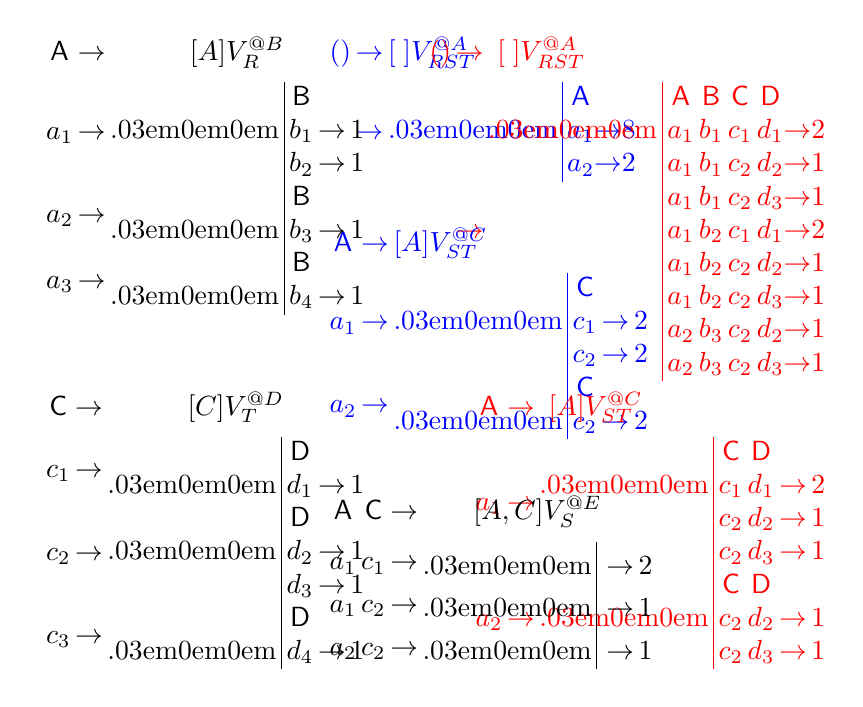
\begin{tikzpicture}[xscale=1.8, yscale=1.01]
  
        % factorized @A
        \node [text=blue, anchor=north west] at (3, 1) {
          \begin{tabular}{@{}l@{\,} @{\,}c@{\,}c@{\,}l@{}}
            & $()$ & $\to$ & $\VIEW[\;]{V^{@A}_{RST}}$ \\[1ex]\toprule 
             & $\tuple{}$ & $\rightarrow$ &
              \begin{tabular}{@{}l@{\,}!{\vrule width 0.03em}@{\,}c@{}c@{}c@{}}
                & $\mathsf{A}$ & & \\
                \specialrule{.03em}{0em}{0em} 
                & $a_1$ & $\rightarrow$ & $8$ \\
                & $a_2$ & $\rightarrow$ & $2$ \\
              \end{tabular}\\\bottomrule 
          \end{tabular}
        };
  
        % flat @A
        \node [text=red, anchor=north east] at (6.7, 1) {
          \begin{tabular}{@{}l@{\,}  @{\,}c@{\,}c@{\,}l@{}}
            & $()$ & $\rightarrow$ & \ $\VIEW[\;]{V^{@A}_{RST}}$ \\[1ex]\toprule
              & $\tuple{}$ & $\rightarrow$ & 
              \begin{tabular}{@{}l@{\,}!{\vrule width 0.03em}@{\,}c@{\,}c@{\,}c@{\,}c@{}c@{}c@{}}
                & $\mathsf{A}$ & $\mathsf{B}$ & $\mathsf{C}$ & $\mathsf{D}$ & & \\
                \specialrule{.03em}{0em}{0em} 
                & $a_1$ & $b_1$ & $c_1$ & $d_1$ & $\rightarrow$ & $2$ \\
                & $a_1$ & $b_1$ & $c_2$ & $d_2$ & $\rightarrow$ & $1$ \\
                & $a_1$ & $b_1$ & $c_2$ & $d_3$ & $\rightarrow$ & $1$ \\
                & $a_1$ & $b_2$ & $c_1$ & $d_1$ & $\rightarrow$ & $2$ \\
                & $a_1$ & $b_2$ & $c_2$ & $d_2$ & $\rightarrow$ & $1$ \\
                & $a_1$ & $b_2$ & $c_2$ & $d_3$ & $\rightarrow$ & $1$ \\
                & $a_2$ & $b_3$ & $c_2$ & $d_2$ & $\rightarrow$ & $1$ \\
                & $a_2$ & $b_3$ & $c_2$ & $d_3$ & $\rightarrow$ & $1$ \\
              \end{tabular}\\\bottomrule
          \end{tabular}
        };
  
        % factorized @C
        \node [text=blue, anchor=north west] at (3, -1.4) {
          \begin{tabular}{@{}l@{\,} @{\,}c@{\,}c@{\,}l@{}}
            & $\mathsf{A}$ & $\rightarrow$ & $\VIEW[A]{V^{@C}_{ST}}$ \\[1ex]\toprule
             & $a_1$ & $\rightarrow$ &
              \begin{tabular}{@{}l@{\,}!{\vrule width 0.03em}@{\,}c@{\,}c@{\,}c@{}}
                & $\mathsf{C}$ & & \\
                \specialrule{.03em}{0em}{0em} 
                & $c_1$ & $\rightarrow$ & $2$ \\
                & $c_2$ & $\rightarrow$ & $2$ \\
              \end{tabular} \\
            \rule{0mm}{4mm} & $a_2$ & $\rightarrow$ &
              \begin{tabular}{@{}l@{\,}!{\vrule width 0.03em}@{\,}c@{\,}c@{\,}c@{}}
                  & $\mathsf{C}$ & & \\
                  \specialrule{.03em}{0em}{0em} 
                  & $c_2$ & $\rightarrow$ & $2$ \\
              \end{tabular}\\\bottomrule 
          \end{tabular}
        };
  
        % flat @C
        \node [text=red, anchor=south east] at (6.7, -7.2) {
          \begin{tabular}{@{}l@{\,} @{\,}c@{\,}c@{\,}l@{}}
            & $\mathsf{A}$ & $\to$ & \ $\VIEW[A]{V^{@C}_{ST}}$ \\[1ex]\toprule
             & $a_1$ & $\rightarrow$ & 
              \begin{tabular}{@{}l@{\,}!{\vrule width 0.03em}@{\,}c@{\,}c@{\,}c@{\,}c@{}}
                & $\mathsf{C}$ & $\mathsf{D}$ & & \\
                \specialrule{.03em}{0em}{0em} 
                & $c_1$ & $d_1$ & $\rightarrow$ & $2$ \\
                & $c_2$ & $d_2$ & $\rightarrow$ & $1$ \\
                & $c_2$ & $d_3$ & $\rightarrow$ & $1$ \\
              \end{tabular}\\
            \rule{0mm}{6mm} & $a_2$ & $\rightarrow$ & 
              \begin{tabular}{@{}l@{\,}!{\vrule width 0.03em}@{\,}c@{\,}c@{\,}c@{\,}c@{}}
                  & $\mathsf{C}$ & $\mathsf{D}$ & & \\
                  \specialrule{.03em}{0em}{0em} 
                  & $c_2$ & $d_2$ & $\rightarrow$ & $1$ \\
                  & $c_2$ & $d_3$ & $\rightarrow$ & $1$ \\
              \end{tabular}\\\bottomrule
          \end{tabular}
        };
  
        % flat/factorized @E
        \node [anchor=south west] at (3, -7.2) {
          \begin{tabular}{@{}l@{\,} @{\,}c@{\,}c@{\,}c@{\,}c@{}}
            %  
            & $\mathsf{A}$ & $\mathsf{C}$ & $\to$ & $\VIEW[A,C]{V^{@E}_{S}}$ \\[1ex]\toprule
             & $a_1$ & $c_1$ & $\rightarrow$ & 
              \begin{tabular}{@{}l@{\,}!{\vrule width 0.03em}@{\,}c@{\,}c@{\,}c@{}}
                & & & \\[-2ex]
                \specialrule{.03em}{0em}{0em} 
                & $\tuple{}$ & $\rightarrow$ & $2$ \\
              \end{tabular} \\
            \rule{0mm}{3mm} & $a_1$ & $c_2$ & $\rightarrow$ & 
              \begin{tabular}{@{}l@{\,}!{\vrule width 0.03em}@{\,}c@{\,}c@{\,}c@{}}
                  & & & \\[-2ex]
                  \specialrule{.03em}{0em}{0em} 
                  & $\tuple{}$ & $\rightarrow$ & $1$ \\
              \end{tabular}\\
            \rule{0mm}{3mm} & $a_2$ & $c_2$ & $\rightarrow$ &
              \begin{tabular}{@{}l@{\,}!{\vrule width 0.03em}@{\,}c@{\,}c@{\,}c@{}}
                  & & & \\[-2ex]
                  \specialrule{.03em}{0em}{0em} 
                  & $\tuple{}$ & $\rightarrow$ & $1$ \\
              \end{tabular}\\\bottomrule
          \end{tabular}
        };
  
        % flat factorized @B
        \node [anchor=north west] at (1, 1) {
          \begin{tabular}{@{}l@{\,} @{\,}c@{\,}c@{\,}c@{}}
            %  
            & $\mathsf{A}$ & $\to$ & $\VIEW[A]{V^{@B}_{R}}$ \\[1ex]\toprule
             & $a_1$ & $\rightarrow$ &
              \begin{tabular}{@{}l@{\,}!{\vrule width 0.03em}@{\,}c@{\,}c@{\,}c@{}}
                & $\mathsf{B}$ & & \\
                \specialrule{.03em}{0em}{0em} 
                & $b_1$ & $\rightarrow$ & $1$ \\
                & $b_2$ & $\rightarrow$ & $1$ \\
              \end{tabular} \\
            \rule{0mm}{4mm} & $a_2$ & $\rightarrow$ &
              \begin{tabular}{@{}l@{\,}!{\vrule width 0.03em}@{\,}c@{\,}c@{\,}c@{}}
                  & $\mathsf{B}$ & & \\
                  \specialrule{.03em}{0em}{0em} 
                  & $b_3$ & $\rightarrow$ & $1$ \\
              \end{tabular} \\
            \rule{0mm}{4mm} & $a_3$ & $\rightarrow$ &
              \begin{tabular}{@{}l@{\,}!{\vrule width 0.03em}@{\,}c@{\,}c@{\,}c@{}}
                  & $\mathsf{B}$ & & \\
                  \specialrule{.03em}{0em}{0em} 
                  & $b_4$ & $\rightarrow$ & $1$ \\
              \end{tabular}\\\bottomrule 
          \end{tabular}
        };
  
        % flat/factorized @D
        \node [anchor=south west] at (1, -7.2) {
          \begin{tabular}{@{}l@{\,} @{\,}c@{\,}c@{\,}c@{}}
            %  
            & $\mathsf{C}$ & $\to$ & $\VIEW[C]{V^{@D}_{T}}$ \\[1ex]\toprule
             & $c_1$ & $\rightarrow$ &
              \begin{tabular}{@{}l@{\,}!{\vrule width 0.03em}@{\,}c@{\,}c@{\,}c@{}}
                  & $\mathsf{D}$ & & \\
                  \specialrule{.03em}{0em}{0em} 
                  & $d_1$ & $\rightarrow$ & $1$ \\
              \end{tabular} \\
            \rule{0mm}{6mm} & $c_2$ & $\rightarrow$ & 
              \begin{tabular}{@{}l@{\,}!{\vrule width 0.03em}@{\,}c@{\,}c@{\,}c@{}}
                & $\mathsf{D}$ & & \\
                \specialrule{.03em}{0em}{0em} 
                & $d_2$ & $\rightarrow$ & $1$ \\
                & $d_3$ & $\rightarrow$ & $1$ \\
              \end{tabular} \\
            \rule{0mm}{4.5mm} & $c_3$ & $\rightarrow$ &
              \begin{tabular}{@{}l@{\,}!{\vrule width 0.03em}@{\,}c@{\,}c@{\,}c@{}}
                  & $\mathsf{D}$ & & \\
                  \specialrule{.03em}{0em}{0em} 
                  & $d_4$ & $\rightarrow$ & $1$ \\
              \end{tabular}\\\bottomrule 
          \end{tabular}
        };
      \end{tikzpicture}
    \end{minipage}
  %}
  \caption{
  Computing the query from Example~\ref{ex:relational_ring} 
  over the database
   in Figure~\ref{fig:count} 
   and the relational ring, where $\forall i\in[12]: p_i=\{ () \to 1 \}$.
   The computation uses 
   the view tree $\tau$
  in Figure~\ref{fig:example_payloads}.
   The red views (rightmost column) have payloads storing the listing representation of the intermediate and final query results. The blue views (top two views in the middle column) encode a factorized representation of these results distributed over their payloads. The remaining (black) views remain the same for both representations.
  }
  \label{fig:factorized_listing_ring}
\end{figure}
  
  

%%%%%%%%%%%%%%%%%%%%%%%%%%%%
We next show how to construct a factorized representation of the query result. In contrast to the scenarios discussed above, this representation is {\em not} available as one payload at the root view, but {\em distributed} over the payloads of all views. This hierarchy of payloads, linked via the keys of the views, becomes the factorized representation. A further difference lies with the multiplication operation. For the listing representation, the multiplication is the Cartesian product. For a given view, it is used to concatenate payloads from its child views. For the factorized representation, we further project away values for all but the marginalized variable. More precisely, for each view $\VIEW[\mathcal{S}]{V^{@X}_{rels}}$ and each of its keys $a_{\mathcal{S}}$, let $\VIEW[\mathcal{T}]{P} = \VIEW[a_\mathcal{S}]{V^{@X}_{rels}}$ be the corresponding payload relation. Then, instead of computing this payload, we compute $\VSUM_{Y\in \mathcal{T}-\{X\}}\VIEW[\mathcal{T}]{P}$ by marginalizing the variables in $\mathcal{T}-\{X\}$ and summing up the multiplicities of the tuples in $\VIEW[\mathcal{T}]{P}$ with the same $X$-value.

\begin{example}
\label{ex:factorized_ring}
We continue Example~\ref{ex:relational_ring}. 
Figure~\ref{fig:factorized_listing_ring} shows the contents of the views with factorized payloads (first two columns in black and blue). 
Each view stores relational payloads that have the schema of the marginalized variable. 
Together, these payloads form a factorized representation over the variable order $\omega$ used to define the view tree in Figure~\ref{fig:example_payloads}. At the top of the factorization, we have a union of two $A$-values: $a_1$ and $a_2$. This is stored in the payloads of (middle) {\color{blue}$\VIEW[\;]{V^{A}_{RST}}$}. The payloads of (middle) {\color{blue}$\VIEW[A]{V^{@C}_{ST}}$} store a union of $C$-values $c_1$ and $c_2$ under $a_1$, and a singleton union of $c_2$ under $a_2$. The payloads of $\VIEW[A]{V^{@B}_R}$ store a union of $B$-values $b_1$ and $b_2$ under $a_1$ and a singleton union of $b_3$ under $a_2$. Note the (conditional) independence of the variables $B$ and $C$ given a value for $A$. This is key to succinctness of factorization. In contrast, the listing representation explicitly materializes all pairings of $B$ and $C$-values for each $A$-value, as shown in the payload of (right) {\color{red}$\VIEW[\;]{V^{A}_{RST}}$}. Furthermore, the variable $D$ is independent of the other variables {\em given} $C$. This is a further source of succinctness in the factorization: Even though $c_2$ occurs under both $a_1$ and $a_2$, the relations under $c_2$, in this case the union of $d_2$ and $d_3$, is only stored once in $\VIEW[C]{V^{@D}_T}$. Each value in the factorization keeps a multiplicity, that is, the number of its derivations from the input data. This is necessary for maintenance. 

This factorization is over a variable order that can be used for all queries with same body and different free variables: As long as their free variables sit on top of the bound variables, the variable order is valid and so is the factorization over it. For instance, if the variable $D$ were not free, then the factorization for the new query would be the same except that we would discard the $D$-values from the payload of the view $\VIEW{V^{@D}_{T}}$.\punto
\end{example}


%%%%%%%%%%%%%%%%%%%%%%%%%%%%

\subsection{Matrix Chain Multiplication}
\label{sec:mcm}

Consider the problem of computing a product of a sequence of matrices $\bm{A}_1, \ldots, \bm{A}_n$ over some ring $\RING$, where matrix $\bm{A}_i[x_i, x_{i+1}]$ has the size $p_{i} \times p_{i+1}$, $i \in [n]$. The product $\bm{A} = \bm{A}_1 \cdots \bm{A}_n$ is a matrix of size $p_1 \times p_{n+1}$ and can be formulated as follows:

\begin{align*}
\bm{A}[x_1, x_{n+1}] = \sum_{x_2 \in[p_2]} \cdots \sum_{x_n\in [p_n]} \prod_{i\in[n]} \bm{A}_i[x_i, x_{i+1}]
\end{align*}

We model a matrix $\bm{A}_i$ as a relation $\VIEW[X_i, X_{i+1}]{A_i}$ with the payload carrying matrix values. The query that computes the matrix $\bm{A}$ is:
\begin{align*}
\VIEW[X_1, X_{n+1}]{A} = \VSUM_{X_2} \cdots \VSUM_{X_n} \VPRODBIG_{i \in [n]} \VIEW[X_i, X_{i+1}]{A_i}
\end{align*}
where each of the lifting functions $\{g_{X_j}\}_{j \in [2,n]}$ maps any key value to payload $\RINGONE\in\RING$.
Different variable orders lead to different evaluation plans for matrix chain multiplication. The optimal variable order corresponds to the optimal sequence of matrix multiplications that minimizes the overall multiplication cost, which is the textbook Matrix Chain Multiplication problem~\cite{Cormen:2009:Algorithms}.

\begin{example}
\label{ex:MCM-factorized-update}
Consider a multiplication chain of $4$ matrices of equal size $p \times p$ encoded as relations $\VIEW[X_i, X_{i+1}]{A_i}$. Let $\mathcal{F} = \{ X_1, X_5 \}$ be the set of free variables and $\omega$ be the variable order $X_1 - X_5 - X_3 - \{ X_2, X_4 \}$, i.e., $X_2$ and $X_4$ are children of $X_3$, with the matrix relations placed below the leaf variables in $\omega$. The view tree $\tau(\omega, \mathcal{F})$ has the following views (from bottom to top; the views at $X_5$ and $X_1$ are equivalent to the view at $X_3$):
\begin{align*}
\VIEW[X_1,X_3]{V^{@X_2}_{A_1A_2}} &= \textstyle\VSUM_{X_2} \VIEW[X_1,X_2]{A_1} \VPROD \VIEW[X_2,X_3]{A_2} \\
\VIEW[X_3,X_5]{V^{@X_4}_{A_3A_4}} &= \textstyle\VSUM_{X_4} \VIEW[X_3,X_4]{A_3} \VPROD \VIEW[X_4,X_5]{A_4} \\
\VIEW[X_1,X_5]{V^{@X_3}_{A_1A_2A_3A_4}} &=\hspace{-0.05em} \textstyle\VSUM_{X_3}\hspace{-0.05em} \VIEW[X_1,X_3]{V^{@X_2}_{A_1A_2}} \hspace{-0.05em}\VPROD\hspace{-0.05em} \VIEW[X_3,X_5]{V^{@X_4}_{A_3A_4}}
\end{align*}
Recomputing these views from scratch for each update to an input matrix takes $\bigO{p^3}$ time. A single-value change in any input matrix causes changes in one row or column of the parent view, and propagating them to compute the final delta view takes $\bigO{p^2}$ time. 
% 
Updates to $\VIEW{A_2}$ and $\VIEW{A_3}$ change every value in $\VIEW{A}$. 
In case of a longer matrix chain, propagating $\VIEW{\delta{A}}$ further requires $\bigO{p^3}$ matrix multiplications, same as recomputation.


We exploit factorization to contain the effect of such changes. For instance, if $\VIEW{\delta{A_2}}$ is a factorizable update  expressible as 
$\VIEW[X_2,X_3]{\delta{A_2}} = \VIEW[X_2]{u} \VPROD \VIEW[X_3]{v}$ (see Section~\ref{sec:factorizable_updates}), then we can propagate deltas more efficiently, as products of 
subexpressions:
\begin{align*}
\quad&\VIEW[X_1,X_3]{\delta{V}^{@X_2}_{A_1A_2}} = \underbrace{\left( \textstyle\VSUM_{X_2} \VIEW[X_1,X_2]{A_1} \VPROD \VIEW[X_2]{u} \right)}_{\VIEW[X_1]{u_2}} \VPROD \VIEW[X_3]{v} \\
&\VIEW[X_1,X_5]{\delta{V}^{@X_3}_{A_1A_2A_3A_4}} = \VIEW[X_1]{u_2} \VPROD \left( \textstyle\VSUM_{X_3} \VIEW[X_3]{v} \VPROD \VIEW[X_3,X_5]{V^{@X_4}_{A_3A_4}} \right)
\end{align*}
Using such factorizable updates enables the incremental computation in $\bigO{p^2}$ time. The final delta is also in factorized form, suitable for further propagation. 

In general, for a chain of $k$ matrices of size $p \times p$, using a binary view tree of the lowest depth, incremental maintenance with factorizable updates takes $\bigO{p^2\log{k}}$ time, while reevaluation takes $\bigO{p^3 k}$ time. The space needed in both cases is $\bigO{p^2 k}$.
\punto
\end{example}

The above example recovers the main idea of LINVIEW~\cite{NEK:SIGMOD:2014}: use factorization in the incremental computation of linear algebra programs where matrix changes are encoded as vector outer products, $\delta{A} = u \TR{v}$. Such rank-$1$ updates can capture many practical update patterns such as perturbations of one complete row or column, or even changes of the whole matrix when the same vector is added to every row or column. \DF generalizes this idea to arbitrary join-aggregate queries. 


	\caption{}\label{figure:rings}
\end{figure}

We remark that $1/2\leq \diam(F_i)\leq 1$, $\diam(S)=2$, and $1\leq \dist(F_i,S)\leq 14=2R$ for $i=1,2$. Thus, $\diam(S)\simeq \diam(F_i)\simeq \dist(F_i,S)\simeq 1$. For $y\in F_1$, $w\in S$, and $z\in F_2$ consider the concatenation $\gamma(y,w,z)$ of the line segments $[y,w]$ and $[w,z]$.  Note that $\gamma(y,w,z)\subset A$ and $\gamma(y,w,z)\in \Gamma(F_1,F_2;A)\cap \mathcal F$ for each $y\in F_1$, $z\in F_2$, and a.e.\ $w\in S$, by the properties of a $P$-family. Indeed, \ref{perturbations:2} and \ref{perturbations:3} imply that for a.e.\ $w\in S$ the segments $[y,w]$ and $[w,z]$ lie in $\mathcal F$. Moreover, the same properties imply that a.e.\ $w\in S$ does not lie in $\partial \mathcal F$. Hence, by \ref{perturbations:4}, the concatenation of the segments $[y,w]$ and $[w,z]$ lies in $\mathcal F$. 

For each fixed $y\in F_i$ consider the map $S\ni w\mapsto \Phi_y(w)= \frac{w-y}{|w-y|}$. By the relative position of $y$ and $S$, this map is uniformly bi-Lipschitz. Thus, if $S'\subset S$ and $\h^{n-1}(S') \geq a$ for some $a>0$, then  $\h^{n-1}( \Phi_y(S'))\gtrsim_n a$.  We note that the implicit constants are independent of the point $y\in F_i$.

Now, let $\rho$ be an admissible function for $\Gamma(F_1,F_2;A)\cap \mathcal F$. We have 
\begin{align*}
\int_{\gamma(y,w,z)} \rho\, ds\geq 1
\end{align*}
for all $y\in F_1$, $z\in F_2$ and a.e.\ $w\in S$. Suppose that for each $y\in F_1$ there exists $S_y\subset S$ with $\h^{n-1}(S_y)\geq \frac{1}{2}\h^{n-1}(S)$ such that we have $$\int_{[y,w]}\rho\, ds \geq 1/2$$
for all $w\in S_y$. Then for the set $D_y= \Phi_y(S_y)$ we have $\h^{n-1}(D_y)\gtrsim_n 1$.  Lemma \ref{lemma:kallunki_koskela} now implies that $$\int \rho^n \gtrsim_n 1. $$

The other case is that there exists $y\in F_1$ such that there exists a subset $S'$ of $S$ with $\h^{n-1}(S')\geq \frac{1}{2}\h^{n-1}(S)$, and 
$$\int_{[y,w]}\rho\, ds < 1/2$$
for each $w\in S'$. This implies that for each $z\in F_2$ and for a.e.\ $w\in S'$ we have $$\int_{[z,w]} \rho\, ds\geq 1/2.$$
As before, Lemma \ref{lemma:kallunki_koskela} gives that 
$$\int \rho^n \gtrsim_n 1.$$ 
Therefore, we have shown that 
$$\md_n(\Gamma(F_1,F_2;A)\cap \mathcal F)  \geq c(n)>0$$
for a uniform constant $c(n)$ depending only on $n$, whenever $R=7r$.

In the general case, let $k\in \N$ be the largest integer such that $R\geq 7^kr$. Consider the rings $A_i=A(0;7^{i-1}r, 7^ir)$, $i\in \{1,\dots,k\}$. By the serial law \ref{m:serial}, we have
\[
\md_n(\Gamma(F_1,F_2;A)\cap \mathcal F)\geq \sum_{i=1}^k \md_n(\Gamma(F_1,F_2;A_i)\cap \mathcal F)\gtrsim_n k \gtrsim_n \log(R/r). \qedhere\]
\end{proof}

\begin{lemma}\label{lemma:path_bound_modulus}
Let $x\in \R^n$, $R>0$, and $\rho\colon \R^n\to [0,\infty]$  be a Borel function with $\rho \in L^n(\R^n)$.
\begin{enumerate}[\upshape(i)]
	\item\label{lemma:path_bound_modulus:i} For $M>0$, let $\Gamma_M$ be the family of paths $\gamma$ that intersect the ball $B(x,R)$ and satisfy $\ell(\gamma)>MR$. Then $\md_n \Gamma_M\to 0$ as $M\to\infty$.\smallskip
	\item\label{lemma:path_bound_modulus:ii}  Let  $\Gamma$ be a path family with $\md_n\Gamma>a$ for some $a>0$ such that each path $\gamma\in \Gamma$ intersects the ball $B(x,R)$. Then there exists a path $\gamma\in \Gamma$ with
\begin{align*}
\int_{\gamma}\, \rho \, ds \leq c(n,a) \left(\int_{B(x,c(n,a)R)} \rho^n \right)^{1/n}\quad \textrm{and}\quad \ell(\gamma)\leq c(n,a)R.
\end{align*}
\end{enumerate}
\end{lemma}


\begin{proof}
Both statements are conformally invariant. Hence, using a conformal transformation, we may assume that $x=0$ and $R=1$. For $M>1$, the family $\Gamma_M$ is contained in the union of the families
\begin{align*}
\Gamma_1&= \{ \gamma: \ell(\gamma)> M \,\,\, \textrm{and}\,\,\, |\gamma|\subset B(0,\sqrt{M})\} \\
\Gamma_2&=\{\gamma: |\gamma|\cap \partial B(0,1)\neq \emptyset \,\,\, \textrm{and}\,\,\, |\gamma|\cap \partial B(0,\sqrt{M})\neq \emptyset \}
\end{align*}
By the subadditivity of modulus, it suffices to show that $\md_n\Gamma_i$ converges to $0$ as $M\to\infty$ for $i=1,2$. The function $M^{-1}\x_{B(0,\sqrt{M})}$ is admissible for $\Gamma_1$, so $\md_n\Gamma_1\leq c(n)M^{-n/2}$. The modulus of $\Gamma_2$ is given by the explicit formula $\md_n\Gamma_2=c(n)( \log \sqrt{M})^{1-n}$;see property \ref{m:ring}. This proves part \ref{lemma:path_bound_modulus:i}.

Now we prove \ref{lemma:path_bound_modulus:ii}. Let $M=M(n,a)$ be sufficiently large, so that $\md_n\Gamma_M<a/2$. Define $\rho_1=\rho \x_{ B(0,M+1)}$ and let $\Gamma_{1}$ be the family of paths $\gamma\in \Gamma$ such that 
\begin{align*}
\int_{\gamma}\, \rho_1 \, ds >  2^{1/n}a^{-1/n} \|\rho_1\|_{L^n(\R^n)}.
\end{align*}
Then the function $$2^{-1/n}a^{1/n}\|\rho_1\|_{L^n(\R^n)}^{-1}\rho_1$$
is admissible for $\Gamma_1$, provided that $\|\rho_1\|_{L^n(\R^n)}\neq 0$, in which case we have $\md_n\Gamma_1 \leq a/2$. If $\|\rho_1\|_{L^n(\R^n)}=0$, then $\md_n\Gamma_1=0$ by property \ref{m:zero_ae}.  Also, let $\Gamma_2$ be the family of paths $\gamma\in \Gamma$ such that $\ell(\gamma)>M$, so $\md_n\Gamma_2\leq \md_n\Gamma_M <a/2$. By the subadditivity of modulus we have 
$\md_n(\Gamma_1\cup \Gamma_2)<a <\md_n\Gamma$. It follows that   $\Gamma\setminus (\Gamma_1\cup \Gamma_2)$ has positive modulus, and in particular it is non-empty. Thus, there exists a path $\gamma\in \Gamma$ with $\ell(\gamma)\leq M$ and 
$$\int_{\gamma}\rho_1\, ds \leq 2^{1/n}a^{-1/n} \|\rho_1\|_{L^n(\R^n)}.$$
Finally, note that $|\gamma|\subset  B(0,M+1)$ since $|\gamma|\cap B(0,1)\neq \emptyset$ and $\ell(\gamma)\leq M$. Thus,
\begin{align*}
\int_{\gamma}\rho\, ds =\int_{\gamma}\rho_1\, ds,
\end{align*}
which completes the proof, with $c(n,a)=\max\{ M(n,a)+1, 2^{1/n}a^{-1/n}\}$. 
\end{proof}

For a continuum $F\subset \R^n$ and $r>0$ we define $F^r$ to be the continuum $F+\br B(0,r)=\{x+y: x\in F, y\in \br B(0,r)\}$. 

\begin{lemma}\label{lemma:fattening}
Let $\mathcal F$ be a family of curve perturbations in $\R^n$. Then for every open set $U\subset \R^n$ and all pairs of non-empty, disjoint continua $F_1,F_2 \subset  U$ we have
\begin{align*}
\md_n (\Gamma(F_1,F_2;U) \cap \mathcal F)=\lim_{r\to 0} \md_n (\Gamma(F_1^r,F_2^r;U) \cap \mathcal F).
\end{align*}
\end{lemma}

Our proof relies on the properties of $P$-families, which is a new concept, but the main ideas originate in the proof of \cite{Vaisala:null}*{Lemma 2}. 

\begin{proof}Note that $\Gamma(F_1,F_2;U)\cap \mathcal F\subset \Gamma(F_1^r,F_2^r;U)\cap \mathcal F$ for every $r>0$, so one inequality is immediate. Also, if $F_i$ is a point $x_0$ for some $i=1,2$, then there exists $R>0$ such that by properties \ref{m:subordinate} and \ref{m:ring} we have
$$\md_n (\Gamma(F_1^r,F_2^r;U) \cap \mathcal F) \leq \md_n \Gamma(A(x_0;r,R))= c(n) \left(\log\frac{R}{r}\right)^{1-n}$$
for all sufficiently small $r>0$. Taking $r\to 0$, we obtain the desired conclusion.

We suppose that $\diam(F_i)>0$ for $i=1,2$. Let $\rho \in L^n(\R^n)$ be admissible for $\Gamma(F_1,F_2;U)\cap \mathcal F$. We will show that for each $q<1$ we have 
$$\int_{\gamma}\rho\, ds \geq q$$
for all sufficiently small $r>0$ and $\gamma\in \Gamma(F_1^r,F_2^r;U)\cap \mathcal F$. This will imply that $$\limsup_{r\to 0} \md_n (\Gamma(F_1^r,F_2^r;U) \cap \mathcal F) \leq q^{-n}\int \rho^n.$$
Letting $q\to 1$ and then infimizing over $\rho$ gives the desired
$$\limsup_{r\to 0} \md_n (\Gamma(F_1^r,F_2^r;U) \cap \mathcal F) \leq \md_n (\Gamma(F_1,F_2;U)\cap \mathcal F).$$


Arguing by contradiction, assume that there exists $0<q<1$ and  $r_k\to 0^+$ such that for each $k\in \N$ there exists a path $\gamma_{r_k}\in \Gamma(F_1^{r_k},F_2^{r_k};U)\cap \mathcal F$ with
$$\int_{\gamma_{r_k}}\rho\, ds < q<1.$$
By passing to a subpath, we assume in addition that $|\gamma_{r_k}|$ is disjoint from $F_1\cup F_2$; here we use property \ref{perturbations:3}. We fix $R_0>0$ such that $F_i^{R_0}\subset U$, $\diam(F_i)>2R_0$ for $i=1,2$, and $F_1^{R_0}\cap F_2^{R_0}=\emptyset$. For each  $r_k<R_0$ and $i=1,2$, there exists $x_{i,k}\in F_i$ such that $|\gamma_{r_k}|$ connects the boundary components of the ring $A_{i,k}=A(x_{i,k};r_k,R_0)$. Note that $F_i$ also connects the boundary components of the ring $A_{i,k}$, since $\diam(F_i)>\diam(A_{i,k})$. By passing to a further subpath, we assume in addition that the endpoints of $\gamma_{r_k}$ lie in the inner boundary components of $A_{i,k}$.

We fix $\varepsilon=(1-q)/2>0$. By Lemma \ref{lemma:loewner} we have that if $r_k<R_0/8$, then
\begin{align*}
\md_n (\Gamma( |\gamma_{r_k}|,F_i; A_{i,k}) \cap \mathcal F)\geq c(n) \log(R_0/r_k) \gtrsim_n 1.
\end{align*}
Lemma \ref{lemma:path_bound_modulus} \ref{lemma:path_bound_modulus:ii} implies that if $r_k$ is sufficiently small, depending on $\varepsilon$, then there exists a path $\gamma_i\in \Gamma( |\gamma_{r_k}|,F_i; A_{i,k}) \cap \mathcal F$ such that 
\begin{align*}
\int_{\gamma_i} \rho\, ds\leq c(n) \left(\int_{B(x_{i,k},c(n)r_k)} \rho^n \right)^{1/n} <\varepsilon.
\end{align*}
We concatenate $\gamma_i$, $i=1,2$, with a suitable subpath of $\gamma_{r_k}$; note that the endpoint of $\gamma_i$ that lies in $|\gamma_{r_k}|$ is not in $\partial \mathcal F$ because it is an interior point of a path of $\mathcal F$. By property \ref{perturbations:4}, the concatenation lies in $\mathcal F$.   In this way, we obtain a path $\gamma \in \Gamma( F_1,F_2;U)\cap \mathcal F$ such that 
$$\int_{\gamma} \rho\, ds \leq \int_{\gamma_{r_k}}\rho\, ds + \int_{\gamma_1}\rho\, ds+\int_{\gamma_2}\rho\, ds<q+2\varepsilon=1.$$  
This contradicts the admissibility of $\rho$. 
\end{proof}
\begin{remark}\label{remark:fattening}
From the proof we see that Lemma \ref{lemma:fattening} is valid more generally for families $\mathcal F$ satisfying \ref{perturbations:3}, \ref{perturbations:4}, and the conclusion of Lemma \ref{lemma:loewner} (or a variant of it, such as Lemma \ref{lemma:loewner_proj}, which uses rectangular instead of spherical rings). Recall that $\mathcal F_*(E)$ always satisfies \ref{perturbations:3} and \ref{perturbations:4}; see Remark \ref{remark:p3p4}.
\end{remark}


Our ultimate preliminary result before the proof of Theorem \ref{theorem:perturbation_family} is the following theorem, which is a version of the Lebesgue differentiation theorem for line integrals.

\begin{theorem}\label{theorem:lebesgue_differentiation_lp}
Let $\rho\colon \R^n\to [-\infty,\infty]$ be a Borel function with $\rho\in L^p_{\loc}(\R^n)$ for some $p>1$. Then there exists a path family $\Gamma_0$ with $\md_p\Gamma_0=0$ such that for every rectifiable path $\gamma\notin \Gamma_0$ we have $\int_{\gamma}|\rho|\, ds<\infty$ and 
\begin{align*}
\lim_{r\to 0} \fint_{B(0,r)} \int_{\gamma+x} \rho\, ds= \int_{\gamma}\rho\, ds.
\end{align*} 
\end{theorem}
\begin{proof}
By the subadditivity of modulus, it suffices to prove the statement for paths $\gamma$ contained in a compact set. Thus, we may assume that $\rho\in L^p(\R^n)$. For continuous functions $\rho$ with compact support the statement is trivially true for all rectifiable paths by uniform continuity. For the general case, for fixed $\lambda>0$ consider the  family  $\Gamma_\lambda$ of rectifiable paths $\gamma$ with $\int_{\gamma} |\rho|\, ds<\infty$ and
$$\limsup_{r\to 0} \left|  \fint_{B(0,r)}\int_{\gamma+x}\rho\, ds -\int_{\gamma} \rho\, ds \right| >\lambda.$$
It suffices to show that $\md_p\Gamma_\lambda=0$ for each $\lambda>0$. Let $\phi$ be a continuous function with compact support. Then,  $\Gamma_{\lambda}\subset \Gamma_1\cup \Gamma_2$, where $\Gamma_1$ is the family of rectifiable paths $\gamma$ with  
\begin{align*}
\limsup_{r\to 0}   \fint_{B(0,r)}\int_{\gamma+x}|\rho-\phi|\, ds >\lambda/2
\end{align*}
and $\Gamma_2$ is the family of rectifiable paths $\gamma$ with
\begin{align*}
\int_{\gamma} |\rho-\phi|\, ds>\lambda/2.
\end{align*}
We note that 
$$\md_p\Gamma_2\leq 2^p\lambda^{-p} \|\rho-\phi\|_{L^p(\R^n)}^p.$$
Moreover, if $\gamma$ is parametrized by arclength, we have
\begin{align*}
 \fint_{B(0,r)}\left(\int_{\gamma+x}|\rho-\phi|\, ds\right)dx = \int_{0}^{\ell(\gamma)} \left(\fint_{B(\gamma(t),r)}|\rho-\phi|\right)\, dt \leq \int_{\gamma}M(\rho-\phi)\, ds,
\end{align*}
where $M(\cdot )$ denotes the centered Hardy--Littlewood maximal function. Hence,
\begin{align*}
\int_{\gamma} M(\rho-\phi)\, ds >\lambda/2
\end{align*}
for $\gamma\in \Gamma_1$. The Hardy--Littlewood maximal $L^p$-inequality \cite{Ziemer:Sobolev}*{Theorem 2.8.2, p.~84} implies that 
\begin{align*}
\md_p\Gamma_1 \leq 2^p \lambda^{-p} \|M(\rho-\phi)\|^p_{L^p(\R^n)} \leq c(n,p) 2^p\lambda^{-p} \|\rho-\phi\|_{L^p(\R^n)}^p.
\end{align*}
Altogether,
\begin{align*}
\md_p\Gamma_{\lambda}\leq \md_p\Gamma_1+\md_p\Gamma_2\lesssim_{n,p,\lambda} \|\rho-\phi\|_{L^p(\R^n)}^p
\end{align*}
Since $\phi$ was arbitrary, we conclude that $\md_p\Gamma_{\lambda}=0$, as desired.
\end{proof}

\begin{proof}[Proof of Theorem \ref{theorem:perturbation_family}]
By the monotonicity of modulus, it suffices to prove that 
\begin{align*}
\md_n \Gamma (F_1,F_2;U) \leq  \md_n (\Gamma(F_1,F_2;U) \cap \mathcal F).
\end{align*}
By Lemma \ref{lemma:fattening}, it suffices to prove that 
\begin{align*}
\md_n \Gamma (F_1,F_2;U) \leq  \md_n (\Gamma(F_1^r,F_2^r;U) \cap \mathcal F)
\end{align*}
for all sufficiently small $r>0$. We fix $r>0$ so that $F_1^r,F_2^r\subset U$. Let $\rho\colon \R^n \to [0,\infty]$ be an admissible function for $\Gamma(F_1^r,F_2^r;U) \cap \mathcal F$ with $\rho\in L^n(\R^n)$. Consider the curve family $\Gamma_0$ with $\md_n\Gamma_0=0$, given by Theorem \ref{theorem:lebesgue_differentiation_lp} and corresponding to $\rho$. Let $\gamma\in \Gamma(F_1,F_2;U)\setminus \Gamma_0$ be a rectifiable path. Since $\mathcal F$ is a family of curve perturbations, by \ref{perturbations:1}, for a.e.\ $x\in B(0,r)$ we have $\gamma+x\in  \Gamma(F_1^r,F_2^r;U) \cap \mathcal F$. Now, the admissibility of $\rho$ for $\Gamma(F_1^r,F_2^r;U) \cap \mathcal F$ and Theorem \ref{theorem:lebesgue_differentiation_lp} imply that $\int_{\gamma}\rho\, ds\geq 1$, so $\rho$ is admissible for $\Gamma(F_1,F_2;U)\setminus \Gamma_0$. Therefore,
\[
\md_n \Gamma (F_1,F_2;U)=\md_n (\Gamma (F_1,F_2;U)\setminus \Gamma_0)\leq \md_n (\Gamma(F_1^r,F_2^r;U) \cap \mathcal F).
\qedhere\]
\end{proof}


\subsection{Examples of families of curve perturbations}\label{section:perturbation:examples}
The next theorem, combined with Theorem \ref{theorem:perturbation_family}, gives Theorem \ref{theorem:cned} \ref{item:cned:ii} and Theorem \ref{theorem:zero}.

\begin{theorem}\label{theorem:perturbation_hausdorff}
Let $E\subset \R^n$ be a set.
\begin{enumerate}[\upshape(i)]
	\item\label{theorem:perturbation_hausdorff:i} If $\h^{n-1}(E)=0$, then $\mathcal F_0(E)$ is a $P$-family.\smallskip
	\item\label{theorem:perturbation_hausdorff:ii} If $E$ has $\sigma$-finite Hausdorff $(n-1)$-measure, then $\mathcal F_{\sigma}(E)$ is a $P$-family. 
\end{enumerate} 
\end{theorem}



The case of Hausdorff $(n-1)$-measure zero, as in \ref{theorem:perturbation_hausdorff:i}, has already been considered by V\"ais\"al\"a \cite{Vaisala:null}*{Lemma 5}, where it is proved that for a.e.\ $x\in \R^n$ we have $\gamma+x\in \mathcal F_0(E)$; that is, \ref{perturbations:1} is satisfied. Recall also that \ref{perturbations:3} and \ref{perturbations:4} are always satisfied for $\mathcal F_0(E)$ and $\mathcal F_{\sigma}(E)$; see Remark \ref{remark:p3p4}. We first prove two preliminary lemmas that will be used in the proof of both cases  \ref{theorem:perturbation_hausdorff:i} and \ref{theorem:perturbation_hausdorff:ii} of the theorem. 

\begin{lemma}\label{lemma:p2}
Let $E\subset \R^n$ and $\gamma$ be a non-constant rectifiable path. For $N\in \N$, let $F_N$ be the set of $x\in \R^n$ such that $E\cap |\gamma+x|$ contains at least $N$ points. Then 
\begin{align*}
m_n^*(F_1)&\leq c(n) \max\{\ell(\gamma),\diam(E)\} \diam(E)^{n-1}\quad \textrm{and}\\
m_n^*(F_N) &\leq c(n) \ell(\gamma)N^{-1} \h^{n-1}(E).
\end{align*}
\end{lemma}
\begin{proof}
%Now, suppose that $\diam(|\gamma|)>4\diam(E)$. Let $x_0\in E$ and $\varepsilon>0$ be such that $\diam(|\gamma|)>4\diam(E)+4\varepsilon$. Consider the ball $B_0=B(x_0,\diam(E) +\varepsilon)$. If $E\cap |\gamma+x|\neq \emptyset$, then $|\gamma+x|\cap \partial B_0\neq \emptyset$ and $|\gamma+x|\cap \partial(2B_0)\neq \emptyset$. Thus, 
%$$\int_{\gamma+x} \x_{2B_0}\, ds \geq \diam(E)+\varepsilon$$
%when $E\cap |\gamma+x|\neq \emptyset$. By Chebychev's inequality and Fubini's theorem, we have
%\begin{align*}
%m_n^*( F_1 ) &\leq m_n\left( \left\{x\in \R^n: \int_{\gamma+x}\x_{2B_0}\, ds\geq \diam(E)+\varepsilon\right\}\right) \\ &\leq (\diam(E)+\varepsilon)^{-1} \int_{\R^n} \int_{\gamma+x} \x_{2B_0}\, ds dx\\&=(\diam(E)+\varepsilon)^{-1} \ell(\gamma)m_n(2B_0)=c(n) \ell(\gamma) (\diam(E)+\varepsilon)^{n-1}.
%\end{align*}
%Finally, we let $\varepsilon\to 0$ to obtain the conclusion.
First we show the second inequality. For $k\in \N$ we define $F_{N,k}$ to be the set of $x\in F_N$ such that $E\cap |\gamma+x|$ contains $N$ points with mutual distances bounded below by $1/k$.  We have $F_{N,k+1} \supset F_{N,k}$, $F_N=\bigcup_{k=1}^\infty F_{N,k}$, and $m_n^*(F_N)=\lim_{k\to\infty}m_{n}^* (F_{N,k})$; see \cite{Bogachev:measure}*{Proposition 1.5.12}. We estimate $m_n^*(F_{N,k})$. We fix a large $k\in \N$ so that $\frac{1}{2k}<{\diam(|\gamma|)}/{4}$. Consider an arbitrary cover of $E$ by sets $U_i$, $i\in I$, with $\diam(U_i)<\frac{1}{2k}$. For each $i\in I$ there exists a closed ball $B_i\supset U_i$ of radius $r_i=\diam(U_i)<\frac{1}{2k}<\diam(|\gamma|)/4$. Define the function 
$$\rho= \frac{1}{N} \sum_{i\in I} \frac{1}{r_i} \x_{2B_i}.$$
If $x\in F_{N,k}$, then $|\gamma+x|$ intersects at least $N$ balls $B_i$ and is not contained in any ball $2B_i$. Therefore,
\begin{align*}
\int_{\gamma+x}\rho\, ds  \geq 1.
\end{align*} 
By Chebychev's inequality and Fubini's theorem, we have
\begin{align*}
m_n^*(F_{N,k}) &\leq\ell(\gamma) \| \rho\|_{L^1(\R^n)}\simeq_n \ell(\gamma) N^{-1} \sum_{i\in I}\diam(U_i)^{n-1}.
\end{align*}
The cover of $E$ by  sets $U_i$, $i\in I$, of diameter less than $\frac{1}{2k}$ was arbitrary, so
$$m_n^*(F_{N,k}) \lesssim_n \ell(\gamma)N^{-1} \mathscr H^{n-1}_{(2k)^{-1}}(E).$$
Letting $k\to \infty$ gives
\[m_n^*(F_N) \lesssim_n \ell(\gamma)N^{-1} \mathscr H^{n-1}(E).\]

For the first inequality, consider two cases. If $\diam(|\gamma|)>4\diam(E)$, then we cover $E$ by a closed ball $B$ of radius $r$ with $0\leq \diam(E)<r<\diam(|\gamma|)/4$. If $x\in F_1$, then $|\gamma+x|$ intersects $B$ and is not contained in $2B$. The above argument for $N=1$ gives $m_n^*(F_1)\lesssim_n \ell(\gamma) r^{n-1}$. Now, we let $r\to \diam(E)$ to obtain $m_n^*(F_1)\lesssim_n \ell(\gamma)\diam(E)^{n-1}$. Next, assume that $\diam(|\gamma|)\leq 4\diam(E)$. In this case, if $x\in F_1$, then $|\gamma+x|\subset \br B(x_0,5\diam(E))$ for a fixed $x_0\in E$. Thus, $m_n^*(F_1)\leq m_n (\br B(x_0,5\diam(E))) =c(n) \diam(E)^n$.
\end{proof}

\begin{lemma}\label{lemma:p3}
Let $E\subset \R^n$, $x\in \R^n$, $r>0$, and for $w\in S^{n-1}(0,1)$ define $\gamma_w(t)=x+tw$, $r/2\leq t\leq r$. For $N\in \N$, let $F_N$ be the set of $w\in S^{n-1}(0,1)$ such that $E\cap |\gamma_w|$ contains at least $N$ points. Then 
\begin{align*}
\h^{n-1}(F_1)&\leq c(n)  r^{-n+1} \min\{r,\diam(E)\}^{n-1}\quad \textrm{and}\\
\h^{n-1}(F_N) &\leq c(n) r^{-n+1}N^{-1} \h^{n-1}(E).
\end{align*}
\end{lemma}
\begin{proof}
For the first inequality, note that $F_1+x$ is equal to the radial projection of $E\cap \{y\in \R^n: r/2\leq |x-y|\leq r\}$ to the sphere $S^{n-1}(x,1)$. This projection is the composition of a uniformly Lipschitz map (projection of $\{y\in \R^n: r/2\leq |x-y|\leq r\}$ to $S^{n-1}(x,r)$) with a scaling by $1/r$. Thus, 
\begin{align*}
\diam(F_1)\lesssim r^{-1} \diam(E\cap \{y\in \R^n: r/2\leq |x-y|\leq r\}) \lesssim r^{-1}\min\{r,\diam(E)\}.
\end{align*}
Moreover, $F_1$ is contained in the intersection of a ball $B_0=\br B(x_0,\diam(F_1))$, where $x_0\in F_1$, with $S^{n-1}(0,1)$. Thus,
\begin{align*}
\h^{n-1}(F_1)\leq \h^{n-1}(B_0\cap S^{n-1}(0,1)) \simeq_n \diam(F_1)^{n-1}.
\end{align*}
This completes the proof of the first inequality.

For the second inequality, we proceed as in the proof of Lemma \ref{lemma:p2}, by defining $F_{N,k}$ to be the set of $w\in S^{n-1}(0,1)$ such that $E\cap |\gamma_w|$ contains $N$ points with mutual distances bounded below by $1/k$. We define the function $\rho$ exactly as in Lemma \ref{lemma:p2}, using an arbitrary cover of $E$ by sets $U_i$ and corresponding balls $B_i\supset U_i$ with $r_i=\diam(U_i)<\frac{1}{2k}<\frac{r}{8}$. Note that if $w\in F_{N,k}$, then 
$$\int_{\gamma_w}\rho\, ds =\int_{r/2}^r \rho( x+tw)\, ds \geq 1.$$
By Chebychev's inequality and polar integration, it follows that 
\begin{align*}
\h^{n-1}( F_{N,k}) &\leq \int_{S^{n-1}(0,1)} \int_{r/2}^r \rho( x+tw)\, dt d\h^{n-1}(w)\\
&\lesssim_n r^{-n+1} \|\rho\|_{L^1(\R^n)} \simeq_n r^{-n+1}  N^{-1} \sum_{i\in I}\diam(U_i)^{n-1}.
\end{align*}
We now proceed as before, infimizing over the covers of $E$ and letting $k\to \infty$. 
\end{proof}

\begin{proof}[Proof of Theorem \ref{theorem:perturbation_hausdorff}]
By Remark \ref{remark:p3p4}, \ref{perturbations:3} and \ref{perturbations:4} are automatically satisfied for $\mathcal F_0(E)$ and $\mathcal F_{\sigma}(E)$. We will establish below properties \ref{perturbations:1} and \ref{perturbations:2}.

Suppose first that $\h^{n-1}(E)=0$ as in \ref{theorem:perturbation_hausdorff:i}. If $\gamma$ is a non-constant rectifiable path, by the second inequality of Lemma \ref{lemma:p2} (for $N=1$) we have that $E\cap |\gamma+x|=\emptyset$, i.e., $\gamma+x\in \mathcal F_0(E)$, for a.e.\ $x\in \R^n$. Hence, \ref{perturbations:1} holds. 

Next, if $x\in \R^n$, $r>0$, and $w\in S^{n-1}(0,1)$, define $\gamma_w(t)=x+tw$, $0\leq t\leq r$. By applying Lemma \ref{lemma:p3} countably many times (for $N=1$) to the paths $\gamma_w|_{[2^{-k}r,2^{-k+1}r ]}$, we have $E\cap \gamma_w([2^{-k}r,2^{-k+1}r ])=\emptyset$ for all $k\in \N$ and for a.e.\ $w\in S^{n-1}(0,1)$. Hence, $E\cap \gamma_w( (0,r])=\emptyset$ for a.e.\ $w\in S^{n-1}(0,1)$. Recall that a path in $\mathcal F_0(E)$, by definition, is allowed to intersect $E$ only at the endpoints. Hence, $\gamma_w\in \mathcal F_0(E)$ for a.e.\ $w\in S^{n-1}(0,1)$. This completes the proof of \ref{perturbations:2} and of  \ref{theorem:perturbation_hausdorff:i}.
    
Next, we suppose that $E$ has $\sigma$-finite Hausdorff $(n-1)$ measure, as in \ref{theorem:perturbation_hausdorff:ii}. We write $E=\bigcup_{k=1}^\infty E_k$, where $\h^{n-1}(E_k)<\infty$ for each $k\in \N$. If we show that $\mathcal F_{\sigma}(E_k)$ is a $P$-family for each $k\in \N$, then $\mathcal F_{\sigma}(E)$ will also be a $P$-family, since the intersection of countably many $P$-families is a $P$-family by Lemma \ref{lemma:intersection}. Hence, for \ref{theorem:perturbation_hausdorff:ii} it suffices to assume that $\h^{n-1}(E)<\infty$. 

Let $\gamma$ be a non-constant rectifiable path. We define $F$ to be the set of $x\in \R^n$ such that $E\cap |\gamma+x|$ is infinite and consider the set $F_N$ as in Lemma \ref{lemma:p2}. Observe that $F=\bigcap_{N=1}^\infty F_N$.  Since 
$$m_n^*(F_N) \lesssim_n \ell(\gamma)N^{-1} \h^{n-1}(E),$$
by letting $N\to \infty$ we obtain $m_n(F)=0$. This proves  \ref{perturbations:1}. 

For \ref{perturbations:2} we fix $x\in \R^n$, $r>0$, and for $w\in S^{n-1}(0,1)$ consider the segment $\gamma_w(t)=x+tw$, $0\leq t\leq r$, as above. For fixed $k\in \N$ we apply Lemma \ref{lemma:p3} to the paths $\gamma_w|_{[2^{-k}r,2^{-k+1}r ]}$ and conclude (by letting $N\to \infty)$ that the set $E\cap \gamma_w([2^{-k}r,2^{-k+1}r ])$ is finite for a.e.\ $w\in S^{n-1}(0,1)$. Hence, for a.e.\ $w\in S^{n-1}(0,1)$ the set $E\cap |\gamma_w|$ is  countable, i.e., $\gamma_w\in \mathcal F_{\sigma}(E)$. 
\end{proof}

\section{Criteria for negligibility}\label{section:criteria}


In this section we prove criteria for the membership of a set $E$ in $\NED$ or $\CNED$. The first of these criteria is crucially used in the proof of Theorem \ref{theorem:unions} regarding the unions of $\NED$ and $\CNED$ sets. Recall that $\*ned$ denotes either $\NED$ or $\CNED$. Also, recall from Section \ref{section:elementary} the definitions of $\*ned(\Omega)$ and $\*ned^w(\Omega)$, and the definition of the relative distance $\Delta(F_1,F_2)$ of two sets $F_1,F_2\subset \R^n$. Let $\gamma\colon [a,b]\to \R^n$ be a non-constant path. If $[c,d]\subset (a,b)$, then the strong subpath $\gamma|_{[c,d]}$ of $\gamma$ is called \textit{strict}.

\begin{theorem}[Main criterion]\label{theorem:criterion_compact}
Let $E\subset \R^n$ be a set such that either $E$ is closed or $m_n(\br E)=0$. The following are equivalent.
\begin{enumerate}[\upshape(I)]
	\item\label{cc:i} $E\in \*ned(\Omega)$ for all open sets $\Omega\subset \R^n$.
	\item\label{cc:ii} $E\in \*ned$.
	\item\label{cc:iii} $E\in \*ned^w(\Omega)$ for some open set $\Omega\subset \R^n$ with $\Omega\supset \br E$.
	\item\label{cc:loewner}There exist constants $t,\phi>0$ such that for each $x_0\in \R^n$ there exists $r_0>0$ with the property that for every pair of non-degenerate, disjoint continua $F_1,F_2\subset B(x_0,r_0)$ with $\Delta(F_1,F_2)\leq t$ we have
\begin{align*}
\md_n(\Gamma(F_1,F_2;\R^n) \cap \mathcal F_*(E)) \geq \phi.
\end{align*}
	\item\label{cc:iv} For each Borel function $\rho\colon \R^n\to [0,\infty]$ with $\rho\in L^n_{\loc}(\R^n)$ there exists a path family $\Gamma_0$ with $\md_n\Gamma_0=0$ such that Conclusion \ref{conclusion:a} below holds for each rectifiable path $\gamma\notin \Gamma_0$ with distinct endpoints. Moreover, $\Gamma_0$ has the property that if $\{\eta_j\}_{j\in J}$ is a finite collection of paths outside $\Gamma_0$ and $\gamma$ is a path with $|\gamma|\subset \bigcup_{j\in J} |\eta_j|$, then $\gamma\notin \Gamma_0$.
	\item\label{cc:v} For each Borel function $\rho\colon \R^n\to [0,\infty]$ with $\rho\in L^n_{\loc}(\R^n)$ there exists a path family $\Gamma_0$ with $\md_n\Gamma_0=0$ such that Conclusion \ref{conclusion:b} below holds for each rectifiable path $\gamma\notin \Gamma_0$ with distinct endpoints.
%	\item\label{cc:vi} $m_n(E)=0$ and part \ref{cc:v} is true for paths $\gamma$ with endpoints not lying in $E$. 
\end{enumerate}	
Moreover, the following implications 
are true for all sets $E\subset \R^n$.
\begin{align*}
\textrm{\ref{cc:iv} $\Rightarrow$ \ref{cc:v}  $\Rightarrow$ \ref{cc:i} $\Rightarrow$ \ref{cc:ii} $\Rightarrow$ \ref{cc:iii} $\Rightarrow$ \ref{cc:loewner} } 
\end{align*}
	
\begin{conclusion}{A}[A$(E,\rho,\gamma)$]\label{conclusion:a}
For each open neighborhood $U$ of $|\gamma|\setminus \partial\gamma$  and for each $\varepsilon>0$ there exists a collection of paths $\{\gamma_i\}_{i\in I}$ and a simple path $\widetilde\gamma$ such that
\begin{enumerate}[\upshape({A}-i)]\smallskip
	\item\label{criterion:i} $\widetilde \gamma \in  \mathcal F_*(E)$,\smallskip
	\item\label{criterion:ii} $\partial \widetilde \gamma=\partial \gamma$, $\displaystyle{|\widetilde \gamma|\setminus \partial \gamma\subset {(|\gamma|\setminus  E)}\cup \bigcup_{i\in I} |\gamma_i| }$, and $\bigcup_{i\in I} |\gamma_i|\subset U$,  
	\item\label{criterion:iii} $\displaystyle{\sum_{i\in I}\ell(\gamma_i)<\varepsilon}$, and \smallskip
	\item\label{criterion:iv} $\displaystyle{\sum_{i\in I} \int_{\gamma_i}\rho\, ds <\varepsilon.}$
\end{enumerate}
The paths $\gamma_i$, $i\in I$, may be taken to lie outside a given path family $\Gamma'$ with $\md_n\Gamma'=0$.  If $\br E\cap \partial \gamma=\emptyset$, then $I$ may be taken to be finite. In general, the trace of each strict subpath of $\widetilde \gamma$ intersects finitely many traces $|\gamma_i|$, $i\in I$.
\end{conclusion}	
	
\begin{conclusion}{B}[B$(E,\rho,\gamma)$]\label{conclusion:b}
For each open neighborhood $U$ of $|\gamma|$ and for each $\varepsilon>0$ there exists a simple path $\widetilde \gamma$ such that
\begin{enumerate}[\upshape({B}-i)]
	\item\label{criterion:bi} $\widetilde \gamma\in \mathcal F_*(E)$,\smallskip
	\item\label{criterion:bii} $\partial \widetilde \gamma=\partial \gamma$ and $|\widetilde \gamma|\subset U$,\smallskip
	\item\label{criterion:biii} $\ell(\widetilde \gamma)\leq \ell(\gamma)+\varepsilon$, and  \smallskip
	\item\label{criterion:biv} $\displaystyle{\int_{\widetilde \gamma} \rho\, ds \leq \int_{\gamma} \rho\, ds +\varepsilon.}$
\end{enumerate}
\end{conclusion}

\end{theorem}
Note that the implications \ref{cc:i} $\Rightarrow$ \ref{cc:ii} $\Rightarrow$ \ref{cc:iii} are trivial. Moreover,  \ref{cc:iii} $\Rightarrow$ \ref{cc:loewner} follows immediately from Lemma \ref{lemma:measure_zero}. Conclusion \ref{conclusion:b} in \ref{cc:v} is only a less technical statement  that follows easily from Conclusion \ref{conclusion:a} in \ref{cc:iv}. Indeed, \ref{criterion:biii} and \ref{criterion:biv} follow from \ref{criterion:ii}, \ref{criterion:iii}, and \ref{criterion:iv}, using Lemma \ref{lemma:paths} \ref{lemma:paths:iv}.  Hence, we will show implications \ref{cc:loewner} $\Rightarrow$ \ref{cc:iv}, which is the most technical one,  and \ref{cc:v} $\Rightarrow$ \ref{cc:i}.

Roughly speaking, Conclusions \ref{conclusion:a} and \ref{conclusion:b} say that with small cost we can alter the path $\gamma$ to bring it inside the curve family $\mathcal F_*(E)$. The assumption that $E$ is closed or $m_n(\br E)=0$ will be crucially used in the proof of \ref{cc:loewner} $\Rightarrow$ \ref{cc:iv} (see Lemma \ref{lemma:exceptional_family}) and it is doubtful whether this implication holds without that assumption.  

An immediate corollary of Theorem \ref{theorem:criterion_compact} is the quasiconformal and bi-Lipschitz invariance of compact $\*ned$ sets.
\begin{corollary}\label{corollary:qc_invariance}
Let $E\subset \R^n$ be a bounded set such that either $E$ is closed or $m_n(\br E)=0$. Let $\Omega\subset \R^n$ be an open set with $\br E\subset \Omega$, and $f\colon \Omega\to \R^n$ be a quasiconformal embedding. If $E\in \*ned$, then $f(E)\in \*ned$. 
\end{corollary}
\begin{proof}
Under either assumption, we have $m_n(\br E)=0$ by Lemma \ref{lemma:measure_zero}. Observe that $f(\br E)=\br{f(E)}$ and that this is a compact subset of $f(\Omega)$ having $n$-measure zero by quasiconformality.  Since $f$ distorts the $n$-modulus of each curve family in $\Omega$ by a bounded multiplicative factor, we see that $f(E)\in \*ned^w (f(\Omega))$.  By Theorem \ref{theorem:criterion_compact}, we conclude that $f(E)\in \*ned$. 
\end{proof}


We also prove an alternative criterion in terms of $P$-families; recall the definition of a $P$-family from Section \ref{section:perturbation}. The result is also true for the case of $\NED$ sets but we do not prove it here to avoid some technicalities.

\begin{theorem}[$P$-family criterion]\label{theorem:criterion_pfamily}
Let $E\subset \R^n$ be a set such that either $E$ is closed or $m_n(\br E)=0$. The following are equivalent.
\begin{enumerate}[\upshape(I)]
	\item\label{cp:i} $E\in \CNED$.
	\item\label{cp:ii} For each Borel function $\rho\colon \R^n\to [0,\infty]$ with $\rho\in L^n(\R^n)$ the following statements are true.
		\begin{enumerate}[\upshape({II}-1)]
			\item\label{cp:ii:i} For each rectifiable path $\gamma$, a.e.\ $x\in \R^n$, and every strong subpath $\eta$ of $\gamma+x$ with distinct endpoints, Conclusion \ref{conclusion:b}$(E,\rho,\eta)$ is true.
			\item\label{cp:ii:ii} For $x\in \R^n$, $0<r<R$, and $w\in S^{n-1}(0,1)$ define $\gamma_{w}(t)=x+tw$, $t\in [r,R]$. Then for $\h^{n-1}$-a.e.\ $w\in S^{n-1}(0,1)$,  and for every strong subpath $\eta$ of $\gamma_w$, Conclusion \ref{conclusion:b}$(E,\rho,\eta)$ is true.
		\end{enumerate}
	\item\label{cp:iii} For each Borel function $\rho\colon \R^n\to [0,\infty]$ with $\rho\in L^n(\R^n)$ there exists a $P$-family $\mathcal F$ such that if $\gamma\in \mathcal F$ is a rectifiable path, then  Conclusion \ref{conclusion:b}$(E,\rho,\eta)$ is true for each strong subpath $\eta$ of $\gamma$ with distinct endpoints.
\end{enumerate}
\end{theorem}



Ahlfors--Beurling  \cite{AhlforsBeurling:Nullsets}*{Theorem 10} proved that if a closed set $E\subset \R^n$ is $\NED$ then any two points in $\R^n\setminus E$ can by joined by a curve in $\R^n\setminus E$ of short length. The analogous statement is true for closed $\CNED$ sets.

\begin{corollary}
Let $E\subset \R^n$ be a closed set with $E\in \CNED$. Then for every $\varepsilon>0$ and points $x,y\in \R^n$ there exists a path $\gamma \in \mathcal F_\sigma(E)$ connecting $x$ and $y$ with $\ell(\gamma)\leq  |x-y|+\varepsilon$.
\end{corollary}

\begin{proof}
Let $x,y\in \R^n$ be distinct points, $\gamma$ be the line segment $[x,y]$, and $\varepsilon>0$. Let $\rho \equiv 0$ and consider the $P$-family $\mathcal F$ given by Theorem \ref{theorem:criterion_pfamily} \ref{cp:iii}. By property \ref{perturbations:1} of the $P$-family $\mathcal F$, for a.e.\ $z\in \R^n$ the path $\gamma+z$ lies in $\mathcal F$. Using spherical coordiantes we see that for a.e.\ $r>0$ and for $\h^{n-1}$-a.e.\ $w\in S^{n-1}(0,1)$ the above is true for $z=rw$. We fix  $r<\varepsilon/5$ such that this is true. Using property \ref{perturbations:2} of a $P$-family, for $\h^{n-1}$-a.e.\ $w\in S^{n-1}(0,1)$ the radial segments $\gamma_w^x(t)= x+tw$ and $\gamma_w^y(t)= y+tw$, $0\leq t\leq r$, lie in $\mathcal F$. Thus, there exists $w\in S^{n-1}(0,1)$ such that both radial segments lie in $\mathcal F$ and $\gamma+rw\in \mathcal F$. We now apply Conclusion \ref{conclusion:b} \ref{criterion:biii} (with $\varepsilon=r$) to each of $\gamma_w^x$, $\gamma_w^y$, and $\gamma+rw$, to conclude that there exist paths $\eta_x,\eta_y,\eta\in\mathcal F_{\sigma}(E)$ with the same endpoints as $\gamma_w^x,\gamma_w^y,\gamma+rw$, respectively, such that $\ell(\eta_x) \leq 2r$, $\ell(\eta_y)\leq 2r$, and $\ell(\gamma+rw) \leq |x-y|+r$. Concatenating these paths gives a path in $\mathcal F_{\sigma}(E)$ connecting $x$ and $y$ with length bounded by $|x-y|+ 5r<|x-y|+\varepsilon$.
\end{proof}


\subsection{Auxiliary results}

We will need some auxiliary results before we prove Theorems \ref{theorem:criterion_compact} and \ref{theorem:criterion_pfamily}. The following lemma is elementary.

\begin{lemma}\label{claim:lambda}
Let $E\subset \R^n$ be a compact set with $m_n(E)=0$, $g\colon \R^n\to [0,\infty]$ be a function in $L^1(\R^n)$, and $\lambda>0$. For each $\varepsilon>0$ there exists $\delta>0$ such that if $0<r<\delta$ and $B_i=B(x_i,r)$,   $i\in \{1,\dots,N\}$, is a family of pairwise disjoint balls centered at $E$, then 
\begin{align*}
\sum_{i=1}^N\int_{\lambda B_i} g<\varepsilon.
\end{align*}
\end{lemma}

\begin{proof}
Let $\lambda,\varepsilon>0$. Since $E$ is compact with $m_n(E)=0$ and $g\in L^1(\R^n)$, there exists $\delta>0$ such that
\begin{align}\label{claim:ineq}
\int_{N_{\lambda \delta}(E)}g<C(n,\lambda)^{-1}\varepsilon 
\end{align}
for a constant $C(n,\lambda)>0$ to be determined. Let $0<r<\delta$ and consider a family of finitely many disjoint balls $B_i=B(x_i,r)$, $i\in \{1,\dots,N\}$, centered at $E$. Suppose that $\lambda>1$. If $x\in \lambda B_i$, then $B_i\subset \lambda B_i\subset B(x,2\lambda r)$. Since the balls $B_i$, $i\in \{1,\dots,N\}$, are disjoint, by volume comparison we see that 
\begin{align*}
\sum_{i=1}^N \x_{\lambda B_i }\leq 2^n\lambda^n \x_{\bigcup_{i=1}^N \lambda B_i} \leq 2^n\lambda^n \x_{N_{\lambda r }(E)}.
\end{align*}
The same inequality is trivially true when $0<\lambda\leq 1$ with constant $1$ in place of $2^n\lambda^n$. We now set $C(n,\lambda)=\max\{1,2^n\lambda^n\}$ and by \eqref{claim:ineq} we  obtain
\[
\sum_{i=1}^N \int_{\lambda B_i} g= \int g \sum_{i=1}^N \x_{\lambda  B_i}\leq C(n,\lambda) \int_{N_{\lambda r}(E)} g<\varepsilon.\qedhere
\]
\end{proof}



\begin{lemma}\label{lemma:exceptional_family}
Let $E\subset \R^n$ be a closed set with $m_n(E)=0$. Then for each non-negative function $\rho\in L^n_{\loc}(\R^n)$  {and for each $\lambda>0$}
\begin{enumerate}[\upshape(i)]
	\item there exists a path family $\Gamma_0$ with $\md_n\Gamma_0=0$ and
	\item\label{lemma:exceptional_family_radii} for each $m\in \N$ there exists a family of balls $\{B_{i,m}=B(x_{i,m}, r_{i,m})\}_{i\in I_m}$ covering $E$ with $r_{i,m}<1/m$, $i\in I_m$,
\end{enumerate}
such that for every non-constant curve $\gamma\notin \Gamma_0$ we have
\begin{align}
\begin{aligned}\label{lemma:exceptional_family_limits}
&\lim_{m\to\infty} \sum_{i: B_{i,m}\cap |\gamma|\neq \emptyset} r_{i,m} \left(\fint_{{\lambda B_{i,m}}} \rho ^n \right)^{1/n}=0\quad \textrm{and}\\
&\lim_{m\to\infty} \sum_{i: B_{i,m}\cap |\gamma|\neq \emptyset} r_{i,m} =0.
\end{aligned}
\end{align}
\end{lemma}




\begin{proof}
First, we reduce to the case that $E$ is compact. Suppose that  the statement is true for compact sets. For $k\in \N$, let $A_k= \{x\in \R^n: k-1\leq |x|\leq k\}$. Then for each $k\in \N$, there exists a curve family $\Gamma_k$ with $\md_n\Gamma_k=0$ and for each $m\in \N$ there exists a family of balls $\{B_{i,m}\}_{i\in I_{m,k}}$ covering $E\cap A_k$, with radii less than $1/m$, so that \eqref{lemma:exceptional_family_limits} is true for non-constant paths $\gamma\notin \Gamma_k$. We discard the balls not intersecting $E\cap A_k$, if any. Let $I_m=\bigcup_{k\in \N}I_{m,k}$ and  $\Gamma_0=\bigcup_{k\in \N}\Gamma_k$. Note that $\md_n\Gamma_0=0$ by the subadditivity of modulus. We claim that \eqref{lemma:exceptional_family_limits} is true for the balls $\{B_{i,m}\}_{i\in I_m}$. 

If $\gamma$ is a non-constant path outside $\Gamma_0$, then $\gamma$ is contained in the union of finitely many sets $A_k$, $k\in \N$. Moreover, there exists $k_0\in \N$ such that $B_{i,m}\cap |\gamma|= \emptyset$ for all $i\in I_{m,k}$, $m\in \N$, and $k>k_0$.  Thus, in \eqref{lemma:exceptional_family_limits}, the sums over the indices $i\in I_{m,k}$ such that $B_{i,m}\cap |\gamma|\neq \emptyset$ are zero for all $k>k_0$. For $k\leq k_0$, the limits of the corresponding sums vanish, since $\gamma\notin \Gamma_k$. Since limits commute with finite sums, we obtain \eqref{lemma:exceptional_family_limits} for the family of balls $\{B_{i,m}\}_{i\in I_m}$. 



Suppose now that $E$ is compact. Let $g\in L^n(\R^n)$ be a non-negative function, to be specified later. By the $5B$-covering lemma (\cite{Heinonen:metric}*{Theorem 1.2}) for each $r>0$ we can find a cover of $E$ by finitely many balls of radius $r$ centered at $E$ so that the balls with the same centers and radius $r/5$ are disjoint. Combining this with Lemma \ref{claim:lambda} (for $5\lambda$ in place of $\lambda$), for each $m\in \N$ we may find a cover of $E$ by balls $B_{i,m}=B(x_{i,m},r_m)$, $i\in I_m$, centered at $E$, such that $r_m<1/m$, the balls $\frac{1}{5}B_{i,m}$ are disjoint, and
\begin{align*}
\sum_{i\in I_m} \int_{\lambda B_{i,m}}g^n <\frac{1}{2^m}.
\end{align*}
For $m\in \N$, we define the Borel function 
$$h_m=  \sum_{i\in I_m }\left(\fint_{\lambda B_{i,m}} g ^n \right)^{1/n} \x_{2 B_{i,m}}.$$
By Lemma \ref{lemma:bojarski}, we have
\begin{align*}
\sum_{m\in \N}\|h_m\|_{L^n(\R^n)} &\lesssim_n \sum_{m\in \N} \left\|\sum_{i\in I_m }\left(\fint_{\lambda B_{i,m}} g^n \right)^{1/n} \x_{\frac{1}{5}B_{i,m}} \right\|_{L^n(\R^n)} \\
&\lesssim_{n,\lambda}  \sum_{m\in \N} \left(\sum_{i\in I_m }\int_{\lambda B_{i,m}} g^n \right)^{1/n}\lesssim_{n,\lambda}  \sum_{m\in \N}\frac{1}{2^{m/n}}<\infty.
\end{align*}
By a variant of Fuglede's lemma  \cite{Vaisala:quasiconformal}*{Theorem 28.1}, there exists a curve family $\Gamma_0$ with $\md_n\Gamma_0=0$ such that for each path $\gamma\notin \Gamma_0$ we have
\begin{align*}
\lim_{m\to\infty}\int_{\gamma} h_m\, ds=0.
\end{align*}
Implicitly we assume that $\Gamma_0$ contains all curves that are not rectifiable.

Note that if $\gamma$ is a non-constant rectifiable curve, $B_{i,m}\cap |\gamma|\neq \emptyset$, and $m$ is sufficiently large so that $\diam(|\gamma|)> 4m^{-1}>4r_{m}$, then $|\gamma|$ is not contained in $2B_{i,m}$, so
$$\int_{\gamma}\x_{2B_{i,m}} \, ds \geq r_{m}.$$
Thus, 
$$\int_{\gamma} h_m\, ds  \geq \sum_{i: B_{i,m}\cap |\gamma|\neq \emptyset} r_{m} \left(\fint_{\lambda B_{i,m}} g ^n \right)^{1/n}.$$
We conclude that if $\gamma$ is a non-constant  curve outside $\Gamma_0$, then 
\begin{align}\label{lemma:exceptional:family:g}
\lim_{m\to\infty}\sum_{i: B_{i,m}\cap |\gamma|\neq \emptyset} r_{m} \left(\fint_{\lambda B_{i,m}} g ^n \right)^{1/n}=0.
\end{align}


We finally set $g=(\rho+1)\x_{B(0,R)}$ in the above manipulations, where $\rho$ is the given function from the statement  and $B(0,R)$ is a large ball containing the compact set $E$. Note that for all large $m\in \N$ we have $\lambda B_{i,m}\subset B(0,R)$ for all $i\in I_m$.  Then for every non-constant curve $\gamma\notin \Gamma_0$ we obtain \eqref{lemma:exceptional_family_limits} from \eqref{lemma:exceptional:family:g}. 
%Observe that when $E$ is compact, all the balls $B_{i,m}$ can be taken to have the same radius $r_m$. 
\end{proof}


\begin{lemma}\label{lemma:iteration}
Let $E\subset \R^n$ be a set, $\rho\colon \R^n \to [0,\infty]$ be a Borel function, and  $\gamma$ be a rectifiable path with distinct endpoints such that $|\gamma|\cap \br E$ is totally disconnected.  If Conclusion \ref{conclusion:a}$(E,\rho,\eta)$   is true for each {strict} subpath $\eta$ of $\gamma$ with distinct endpoints that do not lie in the set $\br E$, then Conclusion \ref{conclusion:a}$(E,\rho,\gamma)$  is also true.  The above statement remains true for Conclusion \ref{conclusion:b} in place of Conclusion \ref{conclusion:a}.
\end{lemma}

\begin{proof}
We only present the argument for Conclusion \ref{conclusion:a} since the argument for Conclusion \ref{conclusion:b} is similar and less technical. Let $U$ be an open neighborhood of $|\gamma|\setminus \partial \gamma$ and $\varepsilon>0$. It suffices to prove that a strong subpath of $\gamma$ with the same endpoints satisfies Conclusion \ref{conclusion:a}. Consider a parametrization $\gamma\colon [a,b]\to \R^n$. Then there exists an open subinterval $J$ of $[a,b]$ such that $\gamma(J)\subset U$ and $\gamma_{\br J}$ has the same endpoints as $\gamma$. Without loss of generality, we assume that $J=(0,1)$ and we denote the path $\gamma|_{[0,1]}$ by $\gamma$.  

Suppose first that $\br E\cap \partial \gamma=\emptyset$. Since $\br E$ is closed, there exist paths $\gamma|_{[0,t_1]}$, $\gamma|_{[t_2,1]}$ that do not intersect $\br E$, and a strict subpath $\eta=\gamma|_{[t_1,t_2]}$ with $\br E\cap \partial \eta=\emptyset$. By assumption, there exists a simple path $\widetilde \eta$ with the same endpoints as $\eta$ and \textit{finitely many} paths $\eta_i$, $i\in I$, inside $U$ as in  Conclusion \ref{conclusion:a}$(E,\rho,\eta)$. Concatenating $\widetilde \eta$ with $\gamma|_{[0,t_1]}$ and $\gamma|_{[t_2,1]}$, and then passing to a simple weak subpath, gives the desired path $\widetilde \gamma$ that verifies Conclusion \ref{conclusion:a}$(E,\rho,\gamma)$. 

Next, suppose that $\br E\cap \partial\gamma\neq \emptyset$. Consider a sequence $a_j\in (0,1)$, $j\in \Z$, such that $a_{j-1}<a_{j}$ for each $j\in \Z$ and $\bigcup_{j\in \Z}[a_{j-1},a_j]=(0,1)$. Let $\gamma^j=\gamma|_{[a_{j-1},a_j]}$, which is a strict subpath of $\gamma$. Since $\gamma((0,1))$ is disjoint from $\{\gamma(0),\gamma(1)\}$,  the points $a_j$ can be chosen so that $\gamma^j$ has distinct endpoints for $j\in \Z$. Since $|\gamma|\cap \br E$ is totally disconnected, we may further choose the points $a_j$ so that $\gamma(a_j)\notin \br E$ for each $j\in \Z$. 

By assumption, the strict subpath $\gamma^j$ of $\gamma$ satisfies  Conclusion \ref{conclusion:a}$(E,\rho,\gamma^j)$ for each $j\in \Z$. Thus, we obtain paths $\widetilde \gamma^j$ and $\gamma_i^j$, $i\in \{1,\dots,N_j\}$, as in the conclusion, for $\varepsilon 2^{-|j|}$ in place of $\varepsilon$,  and such that $\bigcup_{i=1}^{N_j}|\gamma^j_i|\subset U$. In particular, by \ref{criterion:i} we have $\widetilde \gamma^j\in \mathcal F_*(E)$. If $\mathcal F_*(E)=\mathcal F_0(E)$, since the endpoints of $\widetilde \gamma^j$ do not lie in $E$, we have $|\widetilde\gamma^j|\cap E=\emptyset$. By discarding some paths $\gamma_i^j$, we assume that $|\gamma_i^j|$ intersects $|\widetilde \gamma^j|$ for all $i\in \{1,\dots,N_j\}$. 

We consider parametrizations $\widetilde\gamma^j \colon [a_{j-1},a_j]\to U$ with $\widetilde \gamma^j|_{\{a_{j-1},a_j\}}=\gamma^j|_{\{a_{j-1},a_j\}}$, $j\in \Z$. Then we create a curve $\widetilde \gamma\colon [0,1]\to \br U$ such that $\widetilde \gamma((0,1))\subset U$, by concatenating these paths. Namely, we define $\widetilde \gamma(0)=\gamma(0)$, $\widetilde \gamma(1)=\gamma(1)$, and $\widetilde \gamma|_{[a_{j-1},a_j]}= \widetilde \gamma^j$ for $j\in \Z$. Note that $\ell(\widetilde \gamma^j)\leq \ell(\gamma^j)+\varepsilon2^{-|j|}$, which follows from Conclusion \ref{conclusion:a}. We conclude that $\diam( |\widetilde \gamma^j|)\to 0$, as $|j|\to \infty$, so $\widetilde \gamma$ is continuous. By passing to a weak subpath that has the same endpoints, we assume that $\widetilde \gamma$ is simple.

Property \ref{criterion:i} is immediate for $\widetilde \gamma$. Property \ref{criterion:ii} also holds if $\{\gamma_i\}_{i\in I}$ is the family $\{\gamma_i^j\}_{j\in \Z, i\in \{1,\dots,N_j\}}$. Indeed, all these paths are contained in $U$, and by the properties of the paths $\widetilde \gamma^j$ we have
\begin{align*}
|\widetilde \gamma|\setminus \partial \widetilde \gamma &\subset \bigcup_{j\in \Z} |\widetilde \gamma^j| \subset \bigcup_{j\in \Z} \left( (| \gamma^j|\setminus E) \cup \bigcup_{i=1}^{N_j}|\gamma_i^j| \right) \subset (|\gamma|\setminus E)\cup \bigcup_{j\in \Z} \bigcup_{i=1}^{N_j}|\gamma_i^j|.
\end{align*}
Finally, we have
\begin{align*}
\sum_{j\in \Z} \sum_{i=1}^{N_j} \ell(\gamma_i^j)\leq \sum_{j\in \Z} \varepsilon2^{-|j|}  =3\varepsilon \quad \textrm{and}\quad \sum_{j\in \Z} \sum_{i=1}^{N_j}  \int_{\gamma_i^j}\rho\, ds \leq 3\varepsilon.
\end{align*}
Thus \ref{criterion:iii} and \ref{criterion:iv} hold as well. 

Now, we verify the last part of Conclusion \ref{conclusion:a}. The paths $\gamma_{i}^j$ may be taken to lie outside a given curve family $\Gamma'$ with $\md_n\Gamma'=0$, since they were obtained via Conclusion \ref{conclusion:a}. If $\eta$ is a strict subpath of $\widetilde \gamma$, then $|\eta|$ intersects $\bigcup_{i=1}^{N_j} |\gamma_i^j|$ for finitely many $j\in \Z$. Indeed, as $|j|\to \infty$, the paths $\{\gamma_i^j\}_{i\in \{1,\dots,N_j\}}$ have arbitrarily small lengths by the above, and their traces intersect $|\widetilde \gamma^j|$, which is contained in arbitrarily small neighborhoods of the endpoints of $\widetilde \gamma$. Since $|\eta|$ has positive distance from the endpoints of $\widetilde \gamma$, we conclude that  $|\gamma_{i}^j|$ cannot intersect $|\eta|$ if $|j|$ is sufficiently large. This completes the proof.
\end{proof}




\subsection{Proof of main criterion}
As we have discussed, it suffices to show implication   \ref{cc:v} $\Rightarrow$ \ref{cc:i} for all sets $E$, and implication \ref{cc:loewner} $\Rightarrow$ \ref{cc:iv}, which is the most technical one, for sets $E$ that are closed or whose closure has measure zero.

\begin{comment}
\begin{proof}[Proof of Theorem \ref{theorem:criterion_compact}: \ref{cc:v} $\iff$ \ref{cc:vi}]
Suppose that \ref{cc:v} is true. For \ref{cc:vi}, it suffices to show that $m_n(E)=0$. Let $G$ be a Borel subset of $E$ with $m_n(E\setminus G)=0$. Consider the Borel function $\rho=\x_{\R^n\setminus G}=1-\x_G$, which lies in $L^n_{\loc}(\R^n)$. Then there exists a path family $\Gamma_0$ with $\md_n\Gamma_0=0$ such that Conclusion \ref{conclusion:b}$(E,\rho,\gamma)$ is true for all paths $\gamma\notin \Gamma_0$ with distinct endpoints. In particular, by Lemma \ref{modulus:avoid}, this is true for a.e.\ line segment parallel to a given coordinate direction. Let $\gamma$ be such a line segment, so for each $\varepsilon>0$ there exists a path $\widetilde \gamma \in \mathcal F_*(E)\subset \mathcal F_*(G)$ with the same endpoints as $\gamma$ and 
\begin{align*}
\int_{\widetilde \gamma}\rho\, ds\leq \int_{\gamma}\rho\,ds+\varepsilon.
\end{align*}
By Lemma \ref{lemma:paths} \ref{lemma:paths:iii} we have $\int_{\widetilde \gamma}\x_G\, ds=0$ since $|\gamma|\cap G$ is countable. Thus,
\begin{align*}
\ell(\gamma)\leq \ell(\widetilde \gamma) =\int_{\widetilde \gamma}1\, ds =\int_{\widetilde \gamma}\rho\, ds\leq \int_{\gamma}\rho\, ds+\varepsilon= \ell(\gamma) - \int_{\gamma}\x_G\, ds+\varepsilon.
\end{align*}
By letting $\varepsilon\to 0$, we obtain $\int_{\gamma}\x_G\, ds=0$, so $\h^1(|\gamma|\cap G)=0$ by Lemma \ref{lemma:paths} \ref{lemma:paths:iv}. This is true for a.e.\ line segment $\gamma$ parallel to a coordinate direction, so $m_n(G)=0$ by Fubini's theorem. This implies that $m_n(E)=0$, as desired.

Next, suppose \ref{cc:vi} is true. Let $\rho\in L^n_{\loc}(\R^n)$ be a non-negative Borel function. We consider an exceptional curve family $\Gamma_0$ with $\md_n\Gamma_0=0$ such that Conclusion \ref{conclusion:b}$(E,\rho,\gamma)$ is true for paths $\gamma\notin \Gamma_0$ with distinct endpoints not lying in $E$. By enlarging this exceptional family, we assume that if $\gamma\notin \Gamma_0$, then all subpaths of $\gamma$ also do not lie in $\Gamma_0$; see property \ref{m:subpath}. In addition, since $m_n(E)=0$, by property \ref{m:positive_length} we further assume, by enlarging $\Gamma_0$, that for each $\gamma\notin \Gamma_0$ we have $\h^1(|\gamma|\cap E)=0$. In particular, $|\gamma|\cap E$ is totally disconnected. We still require that $\md_n\Gamma_0=0$. Thus, if $\gamma\notin \Gamma_0$, then Conclusion \ref{conclusion:b} is true for every subpath of $\gamma$ with distinct endpoints not lying in $E$. By Lemma \ref{lemma:iteration}, Conclusion \ref{conclusion:b}$(E,\rho,\gamma)$ is also true. This shows \ref{cc:v}.
\end{proof}
\end{comment}

\begin{proof}[Proof of Theorem \ref{theorem:criterion_compact}: \ref{cc:v} $\Rightarrow$ \ref{cc:i}] 
Let $\Omega\subset \R^n$ be an open set and $F_1,F_2\subset \Omega$ be a pair of non-empty, disjoint continua. By the monotonicity of modulus, it suffices to show that
$$\md_n\Gamma(F_1,F_2;\Omega)\leq \md_n(\Gamma(F_1,F_2;\Omega)\cap \mathcal F_*(E)).$$
Let $\rho\in L^n(\R^n)$ be an admissible function for $\Gamma( F_1,F_2;\Omega)\cap \mathcal F_*(E)$. We consider an exceptional curve family $\Gamma_0$ with $\md_n\Gamma_0=0$ as in \ref{cc:v}. Let $\gamma\in \Gamma(F_1,F_2;\Omega)\setminus \Gamma_0$, so Conclusion \ref{conclusion:b}$(E,\rho,\gamma)$ is true. Thus, for any $\varepsilon>0$ there exists a rectifiable path $\widetilde \gamma\in \Gamma(F_1,F_2;\Omega)\cap \mathcal F_*(E)$ with 
$$1\leq \int_{\widetilde \gamma} \rho\, ds \leq \int_{\gamma} \rho\, ds +\varepsilon.$$
Letting $\varepsilon\to 0$ shows that $\rho$ is admissible for $\Gamma(F_1,F_2;\Omega)\setminus \Gamma_0$. Since $\md_n\Gamma_0=0$, the proof is completed.
\end{proof}


\begin{proof}[Proof of Theorem \ref{theorem:criterion_compact}: \ref{cc:loewner} $\Rightarrow$ \ref{cc:iv}]
By the assumption \ref{cc:loewner}, which coincides with the assumption of Lemma \ref{lemma:measure_zero_loewner}, we have $m_n(E)=0$. Therefore, under either of the initial assumptions of Theorem \ref{theorem:criterion_compact}, we have $m_n(E)=0$. Let $\rho\colon \R^n\to [0,\infty]$ be a Borel function in $L^n_{\loc}(\R^n)$.  By Lemma \ref{lemma:exceptional_family}, for each $m\in \N$ there exists a family of balls $\{B_{i,m}\}_{i\in I_m}$ covering the set $\br E$, with radii converging uniformly in $I_m$ to $0$ as $m\to\infty$, and such that \eqref{lemma:exceptional_family_limits} is true for all paths outside an exceptional family with $n$-modulus zero and for a value of $\lambda>0$ to be specified. Let $\Gamma_0$ be the exceptional family of paths $\gamma$ that either do not  satisfy \eqref{lemma:exceptional_family_limits}, or $\h^1(|\gamma|\cap \br E)>0$. By Lemma \ref{lemma:exceptional_family} and property \ref{m:positive_length}, $\md_n\Gamma_0=0$. Note that the path family $\Gamma_0$ has the required property for \ref{cc:iv}, that if $\{\eta_j\}_{j\in J}$ is a finite collection of paths outside $\Gamma_0$ and $\gamma$ is a path with $|\gamma|\subset \bigcup_{j\in J} |\eta_j|$, then $\gamma\notin \Gamma_0$.

We will show that Conclusion \ref{conclusion:a}$(E,\rho,\gamma)$ holds for all paths $\gamma\notin \Gamma_0$ with distinct endpoints. For $\gamma\notin \Gamma_0$, the set $|\gamma|\cap \br E$ is totally disconnected. In view of Lemma \ref{lemma:iteration}, it suffices to show that Conclusion \ref{conclusion:a}$(E,\rho,\eta)$ is true for each subpath $\eta$ of $\gamma$ with distinct endpoints not lying in the closed set $\br E$. By the defining properties of the curve family $\Gamma_0$, all subpaths of $\gamma$ also lie outside $\Gamma_0$. Therefore, it suffices to show that Conclusion \ref{conclusion:a}$(E,\rho,\gamma)$ is true for each path $\gamma\notin \Gamma_0$ with distinct endpoints \textit{not lying in $\br E$}. 

Let $\gamma\notin \Gamma_0$ be a path with distinct endpoints not lying in $\br E$. As a final reduction, we consider a simple weak subpath $\eta$ of $\gamma$ that has the same endpoints. Note that $\eta\notin \Gamma_0$ by the defining properties of $\Gamma_0$ and that is  suffices to show Conclusion \ref{conclusion:a}$(E,\rho,\eta)$, which implies Conclusion \ref{conclusion:a}$(E,\rho,\gamma)$. Hence, we may impose the additional restriction that $\gamma$ is \textit{simple}.

We fix a simple path $\gamma\notin \Gamma_0$ with distinct endpoints not lying in $\br E$, $\varepsilon>0$, and an open neighborhood $U$ of $|\gamma|\setminus \partial \gamma$. We fix an injective parametrization $\gamma\colon [0,1]\to \R^n$ and note that $\gamma(0),\gamma(1)\notin \br E$ and $\gamma((0,1))\subset U$. 

By the compactness of $|\gamma|\cap \br E$ and the assumption \ref{cc:loewner}, there exists a finite cover of $|\gamma|\cap \br E$ by open balls $V_1,\dots,V_L$ such that for every $i\in \{1,\dots,L\}$ and for any non-degenerate, disjoint continua $F_1,F_2\subset 2V_i$, 
\begin{align}\label{theorem:criterion:nedw}
\textrm{if} \,\,\, \Delta(F_1,F_2)\leq t\,\,\, \textrm{then}\,\,\, \md_n (\Gamma(F_1,F_2;\R^n) \cap \mathcal F_*(E)) \geq \phi.
\end{align}
Observe that if a set $D$ intersects $|\gamma|\cap \br E$ and has sufficiently small diameter, namely $\diam(D)\leq \min\{2^{-1}\diam(V_i): i\in \{1,\dots,L\}\}$, then $D\subset 2V_i$ for some $i\in \{1,\dots,L\}$. Hence,  \eqref{theorem:criterion:nedw} holds for any non-degenerate, disjoint continua $F_1,F_2\subset D$. We also fix $a>1$, depending on $t$, so that if $A=A(x;r,ar)$ is any ring and $F_1,F_2\subset \br A$ are disjoint continua connecting the boundary components of $A$, then 
\begin{align*}
\Delta(F_1,F_2) \leq \frac{2}{a-1} \leq t.  
\end{align*}



If $m\in \N$ is fixed and sufficiently large, by \eqref{lemma:exceptional_family_limits} we have
\begin{align}\label{theorem:criterion:sums}
\sum_{i: B_{i,m}\cap |\gamma|\neq \emptyset} r_{i,m} \left(\fint_{\lambda B_{i,m}} \rho^n \right)^{1/n}< \varepsilon \quad \textrm{and}\quad \sum_{i: B_{i,m}\cap |\gamma|\neq \emptyset} r_{i,m}<\varepsilon.
\end{align}
By the compactness of $|\gamma|\cap \br E$, there exists a finite subcollection $D_1,\dots,D_N$ of  $\{B_{i,m}\}_{i\in I_m}$ covering the set $|\gamma|\cap \br E$. We also assume that $D_i$ intersects $|\gamma|\cap \br E$ for each $i\in \{1,\dots,N\}$ and we denote the radius of $D_i$ by $r_i$. Since the endpoints of $\gamma$ do not lie in $\br E$, we have $|\gamma|\cap \br E \subset U$. Thus, 
$$\delta=  \dist(|\gamma|\cap \br E,\partial \gamma\cup \partial U)>0.$$ 
If $m$ is sufficiently large so that $2(a+\lambda)r_i<\delta$ for each $i\in \{1,\dots,N\}$, we have 
\begin{align}\label{theorem:criterion:inclusion}
\bigcup_{i=1}^N  (a+\lambda)D_i\subset U  \quad \textrm{and}\quad \bigcup_{i=1}^N aD_i\cap \partial\gamma=\emptyset.
\end{align}
Finally, we choose an even larger $m$, so that \eqref{theorem:criterion:nedw} holds for any non-degenerate, disjoint continua $F_1,F_2\subset (a+1)D_i$,  $i\in \{1,\dots,N\}$.


We set $\widetilde \gamma_0=\gamma$. We will define inductively simple paths $\widetilde \gamma_k$, $k\in \{0,\dots,N\}$, with the same endpoints as $\gamma$. Once $\widetilde \gamma_{k-1}$ has been defined for some $k\in \{1,\dots,N\}$ and has the same endpoints as $\gamma$, we define $\widetilde \gamma_k$ as follows. If $D_k\cap |\widetilde \gamma_{k-1}|=\emptyset$, then we set $\gamma_k=\emptyset$ (i.e., the empty path) and $\widetilde \gamma_k=\widetilde \gamma_{k-1}$. Suppose $D_k\cap |\widetilde \gamma_{k-1}|\neq \emptyset$. Consider an injective parametrization $\widetilde \gamma_{k-1}\colon [0,1]\to \R^n$. By \eqref{theorem:criterion:inclusion} the endpoints of $\widetilde \gamma_{k-1}$ do not lie in $aD_k$, thus there exist two moments $0<s_1<s_2<1$ such that $\widetilde \gamma_{k-1}(s_1),\widetilde\gamma_{k-1}(s_2)\in \partial D_k$ and $\widetilde\gamma_{k-1}([0,1]\setminus (s_1,s_2))\cap D_k=\emptyset$.  Moreover, there exist moments $s_1'<s_1$ and $s_2'>s_2$ such that $\widetilde \gamma_{k-1}(s_1'),\widetilde \gamma_{k-1}(s_2')\in \partial (aD_k)$, $G_1=\widetilde\gamma_{k-1}([s_1',s_1])\subset \br{aD_k}\setminus {D_k}$ and $G_2=\widetilde\gamma_{k-1}([s_2,s_2']) \subset \br{aD_k}\setminus {D_k}$; see Figure \ref{figure:gamma}. Note that $G_1$ and $G_2$ are disjoint since the path $\widetilde \gamma_{k-1}$ is simple, and that they connect the boundary components of the ring $aD_k\setminus \br{D_k}$.  Since $\Delta(G_1,G_2)\leq t$ (by the choice of $a$) and $G_1,G_2\subset (a+1)D_k$, by \eqref{theorem:criterion:nedw} we have
\begin{align*}
\md_n (\Gamma(G_1,G_2;\R^n)\cap \mathcal F_*(E))\geq \phi.
\end{align*} 
Note that if $\Gamma'$ is a given path family with $\md_n\Gamma'=0$ as in the end of Conclusion \ref{conclusion:a}, then we also have $$\md_n (\Gamma(G_1,G_2;\R^n)\cap \mathcal F_*(E)\setminus \Gamma')\geq \phi.$$
Each path of $\Gamma(G_1,G_2;\R^n)\cap \mathcal F_*(E)\setminus \Gamma'$ intersects the ball $(a+1)D_k$. By Lemma \ref{lemma:path_bound_modulus} there exists a path $\gamma_k \in \Gamma(G_1,G_2;\R^n)\cap \mathcal F_*(E)\setminus \Gamma'$ such that 
\begin{align}\label{theorem:criterion:integral_length}
\int_{\gamma_k}\rho \, ds \lesssim_{n,\phi,a} r_k \left( \fint_{c(n,\phi,a)D_k} \rho^n \right)^{1/n} \quad \textrm{and}\quad \ell(\gamma_k) \leq  c(n,\phi,a)r_k.
\end{align}
We now set $\lambda=c(n,\phi,a)$ and note that $|\gamma_k|\subset (a+\lambda)D_k\subset U$ by \eqref{theorem:criterion:inclusion}. Also, the endpoints of $\gamma_k$ lie in $|\widetilde \gamma_{k-1}|$. We concatenate $\gamma_k$ with suitable subpaths of $\widetilde \gamma_{k-1}$ that do not intersect $D_k$ to obtain a path $\widetilde \gamma_k$ that has the same endpoints as $\gamma$. If necessary, we replace $\widetilde \gamma_k$ with a simple weak subpath that has the same endpoints. By construction we have 
$$|\widetilde \gamma_k|\subset (|\widetilde \gamma_{k-1}|\setminus D_k)\cup (|\gamma_k|\setminus \partial \gamma_k).$$
Inductively, we see that 
\begin{align}\label{theorem:criterion:induction}
|\widetilde\gamma_k|\subset \left(|\gamma| \setminus \bigcup_{i=1}^k D_i \right)\cup \bigcup_{i=1}^{k} (|\gamma_i|\setminus \partial \gamma_i).
\end{align}


\begin{figure}
\centering
	\begin{overpic}[width=.9\linewidth ]{figures/gamma.png}
		\put (3, 29.3) {$\bullet$}
		\put (0,32.3) {$\gamma(0)=\widetilde \gamma_{k-1}(0)$}
		\put (97,43.2) {$\bullet$}
		\put (85,39.3) {$\gamma(1)=\widetilde \gamma_{k-1}(1)$}
		\put (25, 22.8) {$\bullet$}
		\put (36.5, 27.3) {$\bullet$}
		\put (60,30.3) {$\bullet$}
		\put (71.8, 30.3) {$\bullet$}
		\put (55,43.3) {$D_k$}
		\put (65, 51.3 ) {$aD_k$}
		\put (30,25.3) {$G_1$}
		\put (65,31.8) {$G_2$}
		\put (72.5,6) {$\gamma_k$}
		\put (20,53.5) {$\widetilde \gamma_{k-1}$}
	\end{overpic}
	\caption{The construction of $\widetilde \gamma_k$ from $\widetilde \gamma_{k-1}$. }\label{figure:gamma}
\end{figure}

For $k=N$ we obtain a simple path $\widetilde \gamma=\widetilde \gamma_N$ with the same endpoints as $\gamma$. Since $|\gamma|\cap \br E\subset \bigcup_{i=1}^N D_i$, by \eqref{theorem:criterion:induction} we have 
\begin{align}\label{theorem:criterion:induction2}
|\widetilde \gamma| \subset  (|\gamma|\setminus \br E) \cup \bigcup_{i=1}^{N} (|\gamma_i|\setminus \partial \gamma_i) \quad \textrm{and}\quad |\widetilde \gamma|\cap E \subset \bigcup_{i=1}^{N} (|\gamma_i|\setminus \partial \gamma_i)\cap E.
\end{align}
If $\mathcal F_*(E)=\mathcal F_0(E)$, then   $(|\gamma_i|\setminus \partial \gamma_i)\cap E=\emptyset$ since $\gamma_i\in \mathcal F_0(E)$ for each $i\in \{1,\dots,N\}$. Thus, $|\widetilde \gamma|\cap E=\emptyset$ and $\widetilde \gamma\in \mathcal F_0(E)$. If $\mathcal F_*(E)=\mathcal F_{\sigma}(E)$, then $|\widetilde \gamma_i|\cap E$ is countable for each $i\in \{1,\dots,N\}$, so $|\widetilde \gamma|\cap E$ is countable and $\widetilde \gamma\in \mathcal F_{\sigma}(E)$. Thus,  \ref{criterion:i} is satisfied. From \eqref{theorem:criterion:induction2} we obtain immediately
\begin{align*}
|\widetilde \gamma| \subset (|\gamma|\setminus  E) \cup \bigcup_{i=1}^N |\gamma_i|.
\end{align*}
By construction, we have $\bigcup_{i=1}^N|\gamma_i|\subset \bigcup_{i=1}^N (a+\lambda)D_i \subset U$.   Thus, we have established property \ref{criterion:ii}.  Finally, by \eqref{theorem:criterion:sums} and \eqref{theorem:criterion:integral_length} we have 
$$\sum_{i=1}^N \ell(\gamma_i) \lesssim \sum_{i=1}^N r_i \lesssim \varepsilon \,\,\, \textrm{and}\,\,\,
\sum_{i=1}^N \int_{\gamma_i}\rho\, ds \lesssim  \sum_{i=1}^Nr_{i} \left(\fint_{\lambda D_{i}} \rho^n \right)^{1/n}\lesssim \varepsilon.$$
These inequalities address \ref{criterion:iii} and \ref{criterion:iv}. The last part of Conclusion \ref{conclusion:a}, asserting that the collection  $\{\gamma_i\}_i$ is finite, whenever $\br E\cap \partial\gamma=\emptyset$, is also true. 
\end{proof}



\subsection{\texorpdfstring{Proof of $P$-family criterion}{Proof of P-family criterion}}
%The proofs of the implications \ref{cp:i} $\Rightarrow$ \ref{cp:ii} and \ref{cp:iii} $\Rightarrow$ \ref{cp:i} are the same for $\NED$ and $\CNED$ sets.

\begin{proof}[Proof of Theorem \ref{theorem:criterion_pfamily}: \ref{cp:i} $\Rightarrow$ \ref{cp:ii}]
Let $\rho$ be a non-negative Borel function with  $\rho\in L^n(\R^n)$. By Theorem \ref{theorem:criterion_compact} \ref{cc:v}, there exists a path family $\Gamma_0$ with $\md_n\Gamma_0=0$ such that Conclusion \ref{conclusion:b}$(E,\rho,\gamma)$ is true for all paths $\gamma\notin \Gamma_0$ with distinct endpoints. Moreover, by enlarging $\Gamma_0$ while still requiring that $\md_n\Gamma_0=0$, we may assume that if $\gamma\notin \Gamma_0$, then all subpaths of $\gamma$ also have this property; see \ref{m:subpath}.  By Lemma \ref{modulus:avoid}, for each rectifiable path $\gamma$ and for a.e.\ $x\in \R^n$ we have $\gamma+x\notin \Gamma_0$; in particular, the same holds for all strong subpaths of $\gamma+x$, as required in part \ref{cp:ii:i}. Moreover, if $\gamma_w$ is as in \ref{cp:ii:ii}, by the same lemma, for $\h^{n-1}$-a.e.\ $w\in S^{n-1}(0,1)$ the path $\gamma_w$ and all of its strong subpaths lie outside $\Gamma_0$. This completes the proof. 
\end{proof}

\begin{proof}[Proof of Theorem \ref{theorem:criterion_pfamily}: \ref{cp:iii} $\Rightarrow$ \ref{cp:i}]
Let $\rho\in L^n(\R^n)$ be an admissible function for $\Gamma(F_1,F_2;\R^n)\cap \mathcal F_{\sigma}(E)$, where $F_1,F_2$ are disjoint continua. Consider the $P$-family $\mathcal F$ with the given properties; note that $\mathcal F$ depends on $\rho$. Let $\gamma\in \Gamma(F_1,F_2;\R^n)\cap \mathcal F$ be a rectifiable path. By the properties of $\mathcal F$, each strong subpath of $\gamma$ with distinct endpoints, and in particular $\gamma$, satisfies Conclusion \ref{conclusion:b}. Hence, for each $\varepsilon>0$ there exists a rectifiable path $\widetilde \gamma\in \Gamma(F_1,F_2;\R^n) \cap\mathcal F_{\sigma}(E)$ such that 
$$1\leq \int_{\widetilde \gamma}\rho\, ds \leq \int_{\gamma}\rho \, ds+\varepsilon.$$
As $\varepsilon \to 0$, this shows that $\rho$ is admissible for $\Gamma(F_1,F_2;\R^n)\cap \mathcal F$. Hence,
$$\md_n(\Gamma(F_1,F_2;\R^n)\cap \mathcal F) \leq \int \rho^n.$$
Since $\mathcal F$ is a $P$-family, by Theorem \ref{theorem:perturbation_family}, we have
$$\md_n \Gamma(F_1,F_2;\R^n)= \md_n(\Gamma(F_1,F_2;\R^n)\cap \mathcal F)\leq \int \rho^n.$$
Infimizing over $\rho$, gives $\md_n \Gamma(F_1,F_2;\R^n) \leq \md_n (\Gamma(F_1,F_2;\R^n)\cap \mathcal F_{\sigma}(E))$, so $E$ is $\CNED$. 
\end{proof}


For the proof of the last implication \ref{cp:ii} $\Rightarrow$ \ref{cp:iii}, it is crucial that $\mathcal F_{\sigma}(E)$ is closed under concatenations, a fact that is not true for $\mathcal F_0(E)$. Although the result is true for $\mathcal F_0(E)$, the proof is more involved and we only present the argument for $\mathcal F_{\sigma}(E)$.

\begin{proof}[Proof of Theorem \ref{theorem:criterion_pfamily}: \ref{cp:ii} $\Rightarrow$ \ref{cp:iii}]
First, we show that $m_n(E)=0$ in the case that $E$ is closed. Fix an open ball $B$ and consider the Borel function $\rho=(1-\x_E)\x_B$, which lies in $L^n(\R^n)$. By \ref{cp:ii:i}, Conclusion \ref{conclusion:b}$(E,\rho,\gamma)$ is true for a.e.\ line segment $\gamma$ parallel to a given coordinate direction. Let $\gamma$ be such a line segment that is contained in the ball $B$. For each $\varepsilon>0$ there exists a path $\widetilde \gamma \in \mathcal F_{\sigma}(E)$ contained in $B$, with the same endpoints as $\gamma$, and 
\begin{align*}
\int_{\widetilde \gamma}\rho\, ds\leq \int_{\gamma}\rho\,ds+\varepsilon.
\end{align*}
By Lemma \ref{lemma:paths} \ref{lemma:paths:iii} we have $\int_{\widetilde \gamma}\x_E\, ds=0$ since $|\gamma|\cap E$ is countable. Thus,
\begin{align*}
\ell(\gamma)\leq \ell(\widetilde \gamma) =\int_{\widetilde \gamma}1\, ds =\int_{\widetilde \gamma}\rho\, ds\leq \int_{\gamma}\rho\, ds+\varepsilon= \ell(\gamma) - \int_{\gamma}\x_E\, ds+\varepsilon.
\end{align*}
By letting $\varepsilon\to 0$, we obtain $\int_{\gamma}\x_E\, ds=0$, so $\h^1(|\gamma|\cap E)=0$ by Lemma \ref{lemma:paths} \ref{lemma:paths:iv}. This is true for a.e.\ line segment $\gamma$ in $B$ parallel to a coordinate direction, so $m_n(E\cap B)=0$ by Fubini's theorem. The ball $B$ was arbitrary, so $m_n(E)=0$. 

Let $\rho$ be a non-negative Borel function in $L^n(\R^n)$ and let $\mathcal F$ be the family of rectifiable paths $\gamma$ such that Conclusion \ref{conclusion:b}$(E,\rho,\eta)$ holds for each strong subpath $\eta$ of $\gamma$ with distinct endpoints. We show that $\mathcal F$ is a $P$-family. 

First, we see that \ref{perturbations:1} is satisfied. That is, if $\gamma\colon [a,b]\to \R^n$ is a non-constant rectifiable path, then $\gamma+x\in \mathcal F$ for a.e.\ $x\in \R^n$. This is true by the assumption \ref{cp:ii:i}. For \ref{perturbations:2}, we fix $x\in \R^n$ and $R>0$, and we have to show that for a.e.\ $w\in S^{n-1}(0,1)$ the radial segment $\gamma_w(t)=x+tw$, $t\in [0,R]$, lies in $\mathcal F$. By the assumption \ref{cp:ii:ii}, for each $0<r<R$ and for a.e.\ $w\in S^{n-1}(0,1)$ the radial segment $\gamma_w|_{[r,R]}$ lies in $\mathcal F$. For $r_k=2^{-k}R$, $k\in \N$, we see that $\gamma_{w}|_{[r_k,R]}\in \mathcal F$ for a.e.\ $w\in S^{n-1}(0,1)$ and for all $k\in \N$.  We fix $w\in S^{n-1}(0,1)$ such that $\h^1(|\gamma_w|\cap \br E)=0$ and $\gamma_{w}|_{[r_k,R]}\in \mathcal F$ for all $k\in \N$. Since $m_n(\br E)=0$, these statements hold for a.e.\ $w\in S^{n-1}(0,1)$. Our goal is to show that Conclusion \ref{conclusion:b}$(E,\rho,\eta)$ is true for every strong subpath $\eta$ of $\gamma_w$; this will imply that $\gamma_w\in \mathcal F$, as desired. Every \textit{strict} subpath of $\eta$ is a strong subpath of $\gamma_{w}|_{[r_k,R]}$ for some $k\in \N$. Since $\gamma_{w}|_{[r_k,R]}\in \mathcal F$, every strict subpath of $\eta$ satisfies Conclusion \ref{conclusion:b}. Since $|\eta|\cap \br E$ is totally disconnected, we conclude from Lemma \ref{lemma:iteration} that $\eta$ satisfies Conclusion \ref{conclusion:b}.
 
From the definition of $\mathcal F$ it is clear that \ref{perturbations:3} is always satisfied. We finally have to prove \ref{perturbations:4}. Note that  $\mathcal F_*(E)=\mathcal F_{\sigma}(E)$ in \ref{criterion:bi}. Let $\gamma_1,\gamma_2$ be two paths in $\mathcal F$ that have a common endpoint and let $\gamma$ be their concatenation. Consider a strong subpath $\eta$ of $\gamma$ that has distinct endpoints.  Then $\eta$ is either a strong subpath of $\gamma_1$ or $\gamma_2$, or $\eta$ is the concatenation of strong subpaths $\eta_1$ of $\gamma_1$ and $\eta_2$ of $\gamma_2$. In the latter case, which is the nontrivial one, since $\eta_1$ and $\eta_2$ satisfy Conclusion \ref{conclusion:b}, and in particular \ref{criterion:bi}, there exists paths $\widetilde \eta_1, \widetilde \eta_2 \in \mathcal F_{\sigma}(E)$ as in Conclusion \ref{conclusion:b} with the same endpoints as $\eta_1,\eta_2$, by \ref{criterion:bii}. Concatenating $\widetilde \eta_1$ with $\widetilde \eta_2$ gives a path $\widetilde \eta \in \mathcal F_{\sigma}(E)$, which shows that $\eta$ also satisfies Conclusion \ref{conclusion:b}. Thus, $\gamma\in \mathcal F$, as desired. 
\end{proof}




\subsection{Application to Sobolev removability}\label{section:sobolev}
We prove Theorem \ref{theorem:sobolev_intro} as an application  of Theorem \ref{theorem:criterion_compact}. Specifically, we show that closed $\CNED$ sets $E\subset \R^n$ are {removable for continuous $W^{1,n}$ functions}; that is, every continuous function $f\colon \R^n\to \R$ with $f\in W^{1,n}(\R^n\setminus E)$ lies in $W^{1,n}(\R^n)$. 

\begin{comment}
\begin{theorem}\label{theorem:sobolev}
(THIS THEOREM would be more interesting if we could prove it for ANY measurable CNED set; this is true if $f$ is quasiconformal off $E$.)
Let $E\subset \R^n$ be a $\CNED$ set that is either closed or $m_n(\br E)=0$. Let $f\colon \R^n\to \R$ be a Borel function and suppose that there exists a path family $\Gamma_0$ with $\md_n\Gamma_0=0$ satisfying the following conditions.
\begin{enumerate}[\upshape(i)]
	\item $f\circ \gamma$ is continuous for each path $\gamma\notin \Gamma_0$. [Can drop this in case of $\NED$]
	\item There exists a Borel function $\rho_f\colon \R^n\to [0,\infty]$ with $\rho_f\in L^n_{\loc}(\R^n)$ such that 
	$$\h^1_{\infty}(f(|\gamma|\setminus E)) \leq \int_{\gamma}\rho_f\, ds$$
	for each path $\gamma\notin \Gamma_0$. 
\end{enumerate}
Then $f\in W^{1,n}_{\loc}(\R^n)$.
\end{theorem}
\end{comment}

\begin{proof}[Proof of Theorem \ref{theorem:sobolev_intro}]
Let $f\colon \R^n \to \R$ be continuous with $f\in W^{1,n}(\R^n\setminus E)$. Then the classical gradient $\nabla f$ exists almost everywhere in $\R^n\setminus E$. Since $m_n(E)=0$, there exists a Borel representative of $|\nabla f|$ on $\R^n$. By Fuglede's theorem \cite{Vaisala:quasiconformal}*{Theorem 28.2, p.~95}, there exists a curve family $\Gamma_1$ with $\md_n\Gamma_1=0$ such that for each $\gamma\notin \Gamma_1$ we have $\int_{\gamma} |\nabla f|\, ds<\infty$ and the function $f$ is absolutely continuous on every subpath $\gamma|_{[a,b]}$ of $\gamma$ with $\gamma((a,b))\subset \R^n\setminus E$. Moreover,
$$|f(\gamma(b))-f(\gamma(a))| \leq \int_{\gamma|_{(a,b)}}|\nabla f|\, ds.$$
Let $\gamma\colon [a,b]\to \R^n$ be a path outside  $\Gamma_1$. The set $(a,b)\setminus \gamma^{-1}(E)$ is a countable union of disjoint open intervals $(a_i,b_i)$, $i\in \N$. Using the continuity of $f$ and the above inequality, we have
\begin{align}\label{sobolev:ineq1}
\begin{aligned}
m_1( f( |\gamma|\setminus E))&\leq  \sum_{i\in \N}m_1( f( \gamma([a_i,b_i]))) \leq \sum_{i\in \N}( \max_{[a_i,b_i]} f\circ \gamma- \min_{[a_i,b_i]} f\circ \gamma)\\
&\leq \sum_{i\in \N} \int_{\gamma|_{(a_i,b_i)}} |\nabla f|\, ds \leq  \int_{\gamma} |\nabla f|\, ds.
\end{aligned} 
\end{align} 
In particular, if $\gamma\in \mathcal F_{\sigma}(E)\setminus \Gamma_1$, then
\begin{align}\label{sobolev:ineq2}
m_1(f(|\gamma|)) =m_1(f(|\gamma|\setminus E))\leq \int_{\gamma} |\nabla f|\, ds. 
\end{align}

Since $m_n(E)=0$, in order to show that $f\in W^{1,n}(\R^n)$, it suffices to show that there exists a path family $\Gamma_0$ with $\md_n\Gamma_0=0$, such that $f$ is absolutely continuous along each path $\gamma\notin \Gamma_0$. Let $\Gamma_2$ be the path family given by Theorem \ref{theorem:criterion_compact} \ref{cc:iv}, with $\md_n\Gamma_2=0$ and let $\Gamma_0=\Gamma_1\cup \Gamma_2$. We fix a path $\gamma\notin \Gamma_0$  a subpath $\beta= \gamma|_{[a,b]}$. Note that $\beta\notin \Gamma_2$ by the properties of $\Gamma_2$ in Theorem \ref{theorem:criterion_compact} \ref{cc:iv}. Hence, Conclusion \ref{conclusion:a}$(E,|\nabla f|, \beta)$ is true. For each $\varepsilon>0$ there exists a path $\widetilde \beta \in \mathcal F_{\sigma}(E)$ with the same endpoints as $\beta$ and a collection of paths $\beta_i\notin \Gamma_1$, $i\in I$, such that 
$$|\widetilde \beta|\setminus \partial \widetilde \beta \subset (|\beta|\setminus E) \cup \bigcup_{i\in I}|\beta_i|\,\,\, \textrm{and}\,\,\, \sum_{i\in I}\int_{\beta_i}|\nabla f| \, ds< \varepsilon.$$
Thus, using \eqref{sobolev:ineq1} and \eqref{sobolev:ineq2}, we have
\begin{align*}
|f(\beta(b))-f(\beta(a))| &\leq m_1(f(|\widetilde \beta|)) =m_1( f(|\widetilde \beta|\setminus \partial \beta))\\
&\leq m_1( f(|\beta|\setminus E)) + \sum_{i\in I} m_1(f(|\beta_i|))\\
&\leq \int_{\beta} |\nabla f|  \, ds + \sum_{i\in I} \int_{\beta_i} |\nabla f| \, ds\\
&\leq  \int_{\beta} |\nabla f|  \, ds +\varepsilon.
\end{align*}
Letting $\varepsilon\to 0$ shows that $f$ is absolutely continuous along $\gamma$. 
\end{proof}



\section{Unions of negligible sets}\label{section:union}

In this section we prove Theorem \ref{theorem:unions}, which asserts that the union of countably many closed $\NED$ (resp.\ $\CNED$) sets is $\NED$ (resp.\ $\CNED$). The proof is based on Theorem \ref{theorem:criterion_compact} from the preceding section. We first prove an auxiliary lemma.

\begin{lemma}\label{lemma:hausdorf_continua}
Let $G_i$, $i\in \N$, be a sequence of continua in $\R^n$ with $G_i\subset G_{i+1}$, $i\in \N$, and $\sup_{i\in \N} \h^1(G_i)<\infty$. If $G= \bigcup_{i\in \N} G_i$, then $\h^1(\br G\setminus G)=0$. In particular if $\gamma\colon [0,1]\to \br G$ is a rectifiable path and $\rho\colon \R^n\to [0,\infty]$ is a Borel function, then
\begin{align*}
\int_{\gamma}\rho \, ds =\int_{\gamma} \rho \x_G\, ds. 
\end{align*}
\end{lemma}
\begin{proof}
Without loss of generality, $\diam(G_1)>0$. Let $d=\diam(G_1)$ and we fix $k\in \N$. Since $G_k$ is closed, for each $x\in \br G\setminus G \subset \br G\setminus G_k$ there exists $r_x>0$ such that $B(x,r_x)\cap G_k=\emptyset$. By the $5B$-covering lemma (\cite{Heinonen:metric}*{Theorem 1.2}), there exists family of balls $B_i=B(x_i,r_i)$ with $x_i\in \br G\setminus G$ and $r_i<d$, $i\in \N$, such that  $\br G\setminus G\subset \bigcup_{i\in \N} B_i$, the balls $\frac{1}{5}B_i$ are disjoint, and $\frac{1}{5}B_i\cap G_k=\emptyset$ for each $i\in \N$. 

Fix $i\in \N$. Since $x_i\in \br G$, there exists a point $y\in \frac{1}{10}B_i\cap G$. The sequence $\{G_j\}_{j\in \N}$ is increasing, so there exists $j>k$ such that $y\in \frac{1}{10}B_i\cap G_j$. Since $\diam(G_j)\geq d> \diam(\frac{1}{5}B_i)$ and $G_j$ is a continuum,  there exists a connected set in $   \frac{1}{5}B_i\cap G_j$ that connects $\partial B(x_i,r_i/10)$ to $\partial B(x_i,r_i/5)$. In combination with the fact that $\frac{1}{5}B_i\cap G_k=\emptyset$, we obtain
\begin{align*}
\h^1\left( (G\setminus G_k) \cap \frac{1}{5}B_i\right) \geq \h^1\left( G_j\cap \frac{1}{5}B_i\right) \geq r_i/10.
\end{align*}

We now have
\begin{align*}
\h^1_{\infty}(\br  G\setminus G)\leq \sum_{i\in \N} 2r_i \leq 20 \sum_{i\in \N} \h^1\left( (G\setminus G_k) \cap \frac{1}{5}B_i\right)\leq 20 \h^1(G\setminus G_k). 
\end{align*} 
Since $\h^1(G)=\sup_{i\in \N} \h^1(G_i)<\infty$ and $G\setminus G_k$ decreases to $\emptyset$ as $k\to\infty$, we have $\h^1(\br G\setminus G)=\h^1_{\infty}(\br G\setminus G)=0$. This completes the proof of the first statement. The last statement follows from Lemma \ref{lemma:paths} \ref{lemma:paths:iii}.
\end{proof}



\begin{proof}[Proof of Theorem \ref{theorem:unions}]
We split the proof into several parts.

\smallskip
\noindent
\textbf{Initial setup.} 
Define $E=\bigcup_{i\in \N}E_i$ and let $\rho\in L^n_{\loc}(\R^n)$ be a non-negative Borel function. For each $i\in \N$ there exists an exceptional family $\Gamma_i$ with $\md_n\Gamma_i=0$, given by Theorem \ref{theorem:criterion_compact} \ref{cc:iv}. Also by  property \ref{m:positive_length} the family $\Gamma'$ of paths $\gamma$ with $\h^1(|\gamma|\cap E)>0$ has $n$-modulus zero. Define $\Gamma_0= \Gamma'\cup \bigcup_{i\in \N}\Gamma_i$. By the properties of $\Gamma_i$, the path family $\Gamma_0$ has the property that if $\{\eta_j\}_{j\in J}$ is a finite collection of paths outside $\Gamma_0$ and $\gamma$ is a path with $|\gamma|\subset \bigcup_{j\in J} |\eta_j|$, then $\gamma\notin \Gamma_0$. Moreover $|\gamma|\cap E$ is totally disconnected for all paths $\gamma\notin \Gamma_0$. 

Our goal is to show that Conclusion \ref{conclusion:b}$(E,\rho,\gamma)$ is true for each $\gamma\notin \Gamma_0$. By the last part of Theorem \ref{theorem:criterion_compact} and \ref{cc:v}, this suffices for $E$ to be $\*ned$.  We fix a path $\gamma\notin \Gamma_0$ with distinct endpoints, $\varepsilon>0$, and a neighborhood $U$ of $|\gamma|$. It suffices to show Conclusion \ref{conclusion:b} for a weak subpath of $\gamma$ with the same endpoints; also all weak subpaths of $\gamma$ lie outside $\Gamma_0$ by the properties of $\Gamma_0$. Thus, by replacing $\gamma$ with a simple weak subpath, we assume that $\gamma$ is simple and $\gamma\notin \Gamma_0$.

We introduce some notation. Define $\mathcal W_{\sigma}=\bigcup_{m=1}^\infty \N^m$ and $\mathcal W_0=\N$. We use the notation $\mathcal W_*$ for $\mathcal W_{\sigma}$ or $\mathcal W_0$, depending on whether we are working with $\CNED$ or $\NED$ sets, respectively.  Each element $w\in \N^m\subset \mathcal W_{\sigma}$ is called a \textit{word} of \textit{length} $l(w)=m$. For $w\in \mathcal W_0$ we also define $l(w)=w$. The \textit{empty word} $\emptyset$ has length $0$.   

\smallskip
\noindent
\textbf{Induction assumption.} 
Set $\widetilde \gamma_0= \alpha_{\emptyset}=\gamma$ and note that $\alpha_{\emptyset}\notin \Gamma_0$. Let $U_{\emptyset}$ be a neighborhood of $|\alpha_{\emptyset}|\setminus \partial \alpha_{\emptyset}$ with $\diam(U_{\emptyset})\leq 2\diam(|\alpha_{\emptyset}|)$ and $\br{U_{\emptyset}}\subset U$.  Suppose that for $m\geq 0$  we have defined simple paths $\widetilde \gamma_k$, $k\in \{0,\dots,m\}$, and collections of paths $\{\gamma_i\}_{i\in I_w}$ for $l(w)\leq m-1$ such that  
\begin{enumerate}[\upshape({A}-1)]\smallskip
	\item\label{ucc:i} $\widetilde \gamma_k\in \mathcal F_{*}( \bigcup_{i=1}^k E_i)$ for $k\in \{0,\dots,m\}$,\smallskip
	\item\label{ucc:ii}$\partial \widetilde \gamma_k=\partial \gamma$ and  $|\widetilde \gamma_k|\subset |\gamma|\cup \bigcup_{l(w)\leq k-1} \bigcup_{i\in I_w} |\gamma_i|$ for $k\in \{0,\dots,m\}$,\smallskip
	\item\label{ucc:iii} $\sum_{l(w)\leq m-1}\sum_{i\in I_w}\ell(\gamma_i)<\varepsilon$, and\smallskip
	\item\label{ucc:iv} $\sum_{l(w)\leq m-1}\sum_{i\in I_w}\int_{\gamma_i}\rho\, ds<\varepsilon$.	  
\end{enumerate}
Moreover, suppose we have defined the following objects: 
\begin{enumerate}[\upshape({A}-1)]\setcounter{enumi}{4}
	\item\label{ucc:v} Simple paths $\{\alpha_w\}_{l(w)\leq m}$ such that $\{\alpha_{w}\}_{l(w)=k}$ is a collection of parametri\-zations of the closures of the components of $|\widetilde \gamma_k|\setminus (E_1\cup \dots \cup E_{k})$, for each $k\in \{0,\dots,m\}$. In addition, for $l(w)\leq m$, each strict subpath of $\alpha_w$ lies outside $\Gamma_0$. We remark that in the case of $\mathcal W_*=\mathcal W_0$, there is only one component of $|\widetilde \gamma_k|\setminus (E_1\cup \dots \cup E_{k})$ and $\alpha_k=\widetilde \gamma_k$. 
	\item\label{ucc:vi}  Open sets $\{U_w\}_{l(w)\leq m}$ such that $U_w$ is a neighborhood of $|\alpha_w|\setminus \partial \alpha_w$ with $\diam(U_w)\leq 2\diam(|\alpha_w|)$ for $l(w)\leq m$ and the collection $\{U_w\}_{l(w)=k}$ is disjointed for each $k\in \{0,\dots,m\}$. Moreover,  if $m\geq 1$ and $l(w)\leq m-1$, then $U_{(w,j)}\subset U_w$ for $j\in \N$ in the case $\mathcal W_{*}=\mathcal W_{\sigma}$ and $U_{w+1}\subset U_{w}$ in the case $\mathcal W_*=\mathcal W_0$. Finally,   $\br{U_w}$ does not intersect $E_1\cup \dots\cup E_{l(w)}$, except possibly at the endpoints of $\alpha_w$, for $l(w)\leq m$.
\end{enumerate}
Finally, we require the compatibility property
\begin{enumerate}[\upshape({A}-1)]\setcounter{enumi}{6}
	\item\label{ucc:vii}$|\widetilde \gamma_m|\setminus \bigcup_{l(w)=k} U_w= |\widetilde \gamma_k| \setminus \bigcup_{l(w)=k} U_w$ for $k\in \{0,\dots,m\}$.
\end{enumerate}

\smallskip
\noindent
\textbf{Inductive step.} 
We now define $\widetilde \gamma_{m+1}$ as follows.
Fix $w\in \mathcal W_*$ with $l(w)=m$.  By \ref{ucc:v}   each strict subpath $\eta$ of $\alpha_w$ avoids the path family $\Gamma_0$; thus Conclusion \ref{conclusion:a}$(E_{m+1},\rho, \eta )$ is true and $\h^1(|\eta|\cap E_{m+1})=0$. The latter implies that $|\alpha_w|\cap E_{m+1}$ is totally disconnected. By Lemma \ref{lemma:iteration}, Conclusion \ref{conclusion:a}$(E_{m+1},\rho, \alpha_w )$ is true. Thus, for each $\delta_w>0$ there exists a simple path $\widetilde \alpha_w$ and paths $\gamma_i\notin \Gamma_0$, $i\in I_w$, such that 
	\begin{enumerate}[\upshape({A'}-1)]\smallskip
	\item\label{uc':i} $\widetilde \alpha_{w} \in \mathcal F_*(E_{m+1})$,\smallskip
	\item\label{uc':ii} $\partial \widetilde \alpha_{w}=\partial \alpha_{w}$ and $|\widetilde \alpha_{w}|\subset |\alpha_{w}|\cup \bigcup_{i\in I_{w}} |\gamma_{i}|$ and $\bigcup_{i\in I_{w}} |\gamma_{i}| \subset U_{w}$,\smallskip
	\item\label{uc':iii} $\sum_{i\in I_{w}}\ell(\gamma_{i})<\delta_w$, and \smallskip
	\item\label{uc':iv} $\sum_{i\in I_{w}} \int_{\gamma_{i}}\rho\, ds <\delta_w.$\smallskip
\end{enumerate}
If we choose a sufficiently small $\delta_w$, we can ensure that \ref{ucc:iii} and \ref{ucc:iv} are true for the index $m+1$ in place of $m$. By \ref{uc':ii}, the path $\widetilde \alpha_w$ is obtained by modifying $\alpha_w$ within $U_w$.  By \ref{ucc:vi}, $\br{U_w}$ does not intersect $E_1\cup \dots\cup E_m$, except possibly at the endpoints of $\alpha_w$. Therefore, $\widetilde \alpha_w\in \mathcal F_{*}(E_1\cup\dots\cup E_{m})$. Combining this with \ref{uc':i}, we obtain $\widetilde \alpha_w\in \mathcal F_{*}(E_1\cup\dots\cup E_{m+1})$. 

\begin{figure}
\centering
	\begin{overpic}[width=.7\linewidth]{figures/union_ned.png}
		\put (2, 26.5) {$\bullet$}
		\put (96,26.5) {$\bullet$}
		\put (90,51) {$U_m$}
		\put (84, 45) {$U_{m+1}$}
		\put (51,38) {$\widetilde \gamma_{m+1}$}
		\put (55,20) {$\widetilde \gamma_m$}
	\end{overpic}
	\begin{overpic}[width=.99\linewidth]{figures/union_cned.png}
		\put (90,51) {$U_w$}
		\put (50, 45) {$U_{(w,j)}$}
		\put (50,36) {$ \alpha_{(w,j)}$}
		\put (55,18) {$ \alpha_w$}
	\end{overpic}
	\caption{Construction of $\widetilde \gamma_{m+1}$ from $\widetilde \gamma_m$. Top figure: the case of $\mathcal W_0$. Bottom figure: the case of $\mathcal W_{\sigma}$. The red curve is $\widetilde \alpha_w$ and the green points denote the set $(|\widetilde \gamma_{m+1}|\cap E_{m+1})\cap U_w$, which is countable. In fact, a large part of $\widetilde \alpha_w$ should be shared with $\alpha_w$ by \ref{uc':ii} but we do not indicate this to simplify the figure.}\label{figure:union}
\end{figure}

Using \ref{ucc:v}, we define $\widetilde \gamma_{m+1}$ by replacing each $\alpha_w$ in $\widetilde \gamma_m$, where $l(w)=m$, with $\widetilde \alpha_w$; see Figure \ref{figure:union}. In the case of $\mathcal W_{\sigma}$, we  need to ensure that this procedure gives a path. Indeed, by \ref{uc':ii} and \ref{uc':iii} we have $\ell(\widetilde \alpha_w)\leq \ell(\alpha_w)+\delta_w$, so if $\delta_w$ is sufficiently small, then we obtain a path $\widetilde \gamma_{m+1}$. By \ref{ucc:v}, the endpoints of $\widetilde \gamma_m$ do not lie in $|\alpha_w|\setminus \partial \alpha_w$ for any $w$ with $l(w)=m$, so they are not modified. Thus, $\widetilde \gamma_{m+1}$ has the same endpoints as $\gamma$. Moreover, by \ref{ucc:vi}, the regions $\{U_w\}_{l(w)=m}$, where the paths $\widetilde \alpha_w$ differ from $\alpha_w$ are pairwise disjoint. Hence $\widetilde \gamma_{m+1}$ is a simple path, since $\widetilde \gamma_m$ is simple. 

We now verify \ref{ucc:i} and \ref{ucc:ii}. By construction and \ref{ucc:v}, we have
$$|\widetilde \gamma_{m+1}|\setminus \bigcup_{l(w)=m}(|\widetilde \alpha_w|\setminus \partial \widetilde \alpha_w)= |\widetilde \gamma_m| \setminus \bigcup_{l(w)=m} (|\alpha_w|\setminus \partial \alpha_w) = \partial \gamma \cup  \left(|\widetilde \gamma_m|\cap \bigcup_{i=1}^m E_i\right).$$
In the case of $\mathcal W_{\sigma}$, since $\widetilde \gamma_m\in \mathcal F_{\sigma}(E_1\cup\dots\cup E_m)$ and $\widetilde \alpha_w\in \mathcal F_{\sigma}(E_1\cup\dots\cup E_{m+1})$ for $l(w)=m$,  
we conclude that 
$\widetilde \gamma_{m+1}\in \mathcal F_{\sigma}(E_1\cup\dots\cup E_{m+1})$, as required in \ref{ucc:i}. In the case $\mathcal W_*=\mathcal W_0$ we simply have $\widetilde \gamma_m=\alpha_m$ (see \ref{ucc:v}) and $\widetilde \gamma_{m+1}=\widetilde \alpha_m$, so $\widetilde \gamma_{m+1}\in \mathcal F_0(E_1\cup \dots\cup E_{m+1})$, as desired.  By construction and \ref{uc':ii} we have
\begin{align*}
|\widetilde \gamma_{m+1}| \subset |\widetilde \gamma_m|\cup \bigcup_{l(w)=m}\bigcup_{i\in I_w}|\gamma_i|.
\end{align*}
Thus, by the induction assumption we obtain \ref{ucc:ii} for the index $m+1$. 

Since $\widetilde \gamma_{m+1}$ is obtained by modifying $\widetilde \gamma_m$ in the open sets $U_w$, $l(w)=m$, we have $$|\widetilde \gamma_{m+1}|\setminus \bigcup_{l(w)=m}U_w =|\widetilde \gamma_{m}|\setminus \bigcup_{l(w)=m}U_w.$$
By \ref{ucc:vi}, for $k\leq m$ we have $\bigcup_{l(w)=k}U_w\supset \bigcup_{l(w)=m}U_w$, so 
$$|\widetilde \gamma_{m+1}|\setminus \bigcup_{l(w)=k}U_w= |\widetilde \gamma_m| \setminus \bigcup_{l(w)=k}U_w=  |\widetilde \gamma_k| \setminus \bigcup_{l(w)=k}U_w,$$
where the last equality follows from the induction assumption \ref{ucc:vii}.  This proves the equality in \ref{ucc:vii} for the index $m+1$. 

Next, we verify \ref{ucc:v}. Note that the paths $\{\widetilde \alpha_w\}_{l(w)=m}$, parametrize the closures of the components of $|\widetilde \gamma_{m+1}|\setminus (E_1\cup \dots \cup E_m)$; this follows from the construction and \ref{ucc:v}. For $l(w)=m$, let $\{\alpha_{(w,j)}\}_{j\in \N}$ be a collection of simple paths parametrizing the closures of the components of $|\widetilde \alpha_w|\setminus E_{m+1}$; see Figure \ref{figure:union}. Then $\{\alpha_w\}_{l(w)=m+1}$ gives a collection that parametrizes the closures of the components of $|\widetilde\gamma_{m+1}|\setminus (E_1\cup \dots \cup E_{m+1})$. This verifies the first part of \ref{ucc:v}. Moreover, if $\mathcal W_*=\mathcal W_{\sigma}$, for $l(w)=m$ and $j\in \N$, each strict subpath $\widetilde \eta$ of  $\alpha_{(w,j)}$ is a strict subpath of $\widetilde \alpha_w$. If $\mathcal W_*=\mathcal W_0$, each strict subpath $\widetilde \eta$ of  $\alpha_{w+1}$  is a strict subpath of $\widetilde \alpha_w$. In either case, by \ref{uc':ii}, there exists a strict subpath $\eta$ of $\alpha_w$ such that $|\widetilde \eta|\subset |\eta|\cup \bigcup_{i\in I_w}|\gamma_i|$. By the induction assumption \ref{ucc:v}, $\eta\notin \Gamma_0$. By the last part of Conclusion \ref{conclusion:a} (see the statement in Theorem \ref{theorem:criterion_compact}), $|\widetilde \eta|$ intersects finitely many of the traces $|\gamma_i|$, $i\in I_w$. Recall that $\gamma_i\notin \Gamma_0$, $i\in I_w$. The properties of the family $\Gamma_0$ imply that $\widetilde \eta\notin \Gamma_0$. This completes the proof of the second part of \ref{ucc:v}.

We now discuss \ref{ucc:vi}. If $\mathcal W_*=\mathcal W_0$, we define $U_{m+1}$ to be a neighborhood of $|\alpha_{m+1}|\setminus \alpha_{m+1}$ such that $\diam(U_{m+1})\leq 2\diam(|\alpha_{m+1}|)$, $U_{m+1}\subset U_m$, and $\br{U_{m+1}}$ does not intersect $E_1\cup \dots\cup E_{m+1}$, except possibly at the endpoints of $\alpha_{m+1}$; this uses that $E_1\cup \dots \cup E_{m+1}$ is closed and does not intersect $|\alpha_{m+1}|$, except possibly at the endpoints. If $\mathcal W_*=\mathcal W_{\sigma}$, for $l(w)=m$ we define $U_{(w,1)}$ to be a neighborhood of $|\alpha_{(w,1)}|\setminus  \partial \alpha_{(w,1)}$ such that $\diam(U_{(w,1)})\leq 2\diam(|\alpha_{(w,1)}|)$, $U_{(w,1)}\subset U_w$, and $\br {U_{(w,1)}}$ does not intersect $E_1\cup \dots \cup E_{m+1}$, except possibly at the endpoints of $\alpha_{(w,1)}$. Moreover, since $\alpha_{w}$ is simple, we may require that $\br{U_{(w,1)}}$ is disjoint from $|\alpha_{(w,j)}|\setminus \partial \alpha_{(w,j)}$ for $j>1$. Next, we define $U_{(w,2)}$ to  be a neighborhood of $|\alpha_{(w,2)}|\setminus \partial \alpha_{(w,2)}$ with the same properties as $U_{(w,1)}$ and with $U_{(w,1)}\cap U_{(w,2)}=\emptyset$.  Inductively, we define $U_{(w,j)}$ for all $j\in \N$ with the desired properties; see Figure \ref{figure:union}. We have completed the proof of the inductive step.

\smallskip
\noindent
\textbf{Completion of the proof.} 
Now we will show that Conclusion \ref{conclusion:b}$(E,\rho,\gamma)$ is true. For $m\in \N$ define $G_m=\bigcup_{k=0}^m|\widetilde \gamma_k|$. This is a continuum, since $|\widetilde \gamma_k|$ contains the endpoints of $\gamma$ for each $k\in \N$ by \ref{ucc:ii}. We have $G_{m}\subset G_{m+1}$ and 
\begin{align*}
G_m \subset |\gamma|\cup \bigcup_{l(w)\leq m-1} \bigcup_{i\in I_w} |\gamma_i|
\end{align*}
for $m\in \N$. 
By Lemma \ref{lemma:paths} \ref{lemma:paths:iv} and property \ref{ucc:iii}   we have
\begin{align*}
\h^1(G_m) &\leq \ell(\gamma) + \sum_{l(w)\leq m-1} \sum_{i\in I_w}\ell(\gamma_{i})\leq \ell(\gamma)+\varepsilon.
\end{align*} 
Thus $\sup_{m\in \N} \h^1(G_m)<\infty$, as required in Lemma \ref{lemma:hausdorf_continua}. We set $G=\bigcup_{m\in \N}G_m$. 


Since $\widetilde \gamma_m$ is a simple path for each $m\in \N$, by Lemma \ref{lemma:paths} \ref{lemma:paths:iv}  we have
\begin{align*}
\ell(\widetilde \gamma_m)&= \h^1(|\widetilde \gamma_m|) \leq \h^1(G_m)\leq \ell(\gamma)+\varepsilon.
\end{align*} 
By the Arzel\`a--Ascoli theorem, there exists a subsequence of $\widetilde \gamma_m$, parametrized by arclength, that converges uniformly to a path $\widetilde \gamma$ with the same endpoints as $\gamma$ and 
$$\ell(\widetilde \gamma) \leq \liminf_{m\to\infty}\ell(\widetilde \gamma_m)\leq \ell(\gamma)+\varepsilon.$$
Hence, \ref{criterion:biii} holds.   Since $|\widetilde\gamma_m| \subset \br{U_{\emptyset}}$ for each $m\in \N$ by \ref{ucc:vi}, we have $|\widetilde \gamma|\subset  \br{U_{\emptyset}}\subset U$, as required in \ref{criterion:bii}. We assume that $\widetilde \gamma$ is simple by considering a weak subpath if necessary.  Since $|\widetilde \gamma|\subset \br G$, by Lemma \ref{lemma:hausdorf_continua} and Lemma \ref{lemma:paths} \ref{lemma:paths:iv} we have 
\begin{align*}
\int_{\widetilde \gamma}\rho\, ds &= \int_{\widetilde \gamma}\rho \x_G\, ds = \int_{|\widetilde \gamma|\cap G}\rho\, d\h^1 \leq \int_G \rho\, d\h^1\\
&\leq \int _{\gamma}\rho \, ds + \sum_{w\in \mathcal W_*}\sum_{i\in I_w} \int_{\gamma_{i}}\rho\, ds \leq \int_{\gamma}\rho\, ds + \varepsilon,
\end{align*}
where the last inequality follows from \ref{ucc:iv}. This shows \ref{criterion:biv}. 

Finally, we argue for \ref{criterion:bi}. By \ref{ucc:vii}  for $m\geq k\geq 0$ we have
\begin{align}\label{union:inclusion_mk}
|\widetilde \gamma_m| \subset |\widetilde \gamma_k| \cup  \br{\bigcup_{l(w)=k} U_{w}}.
\end{align}
By \ref{ucc:vi},  $\diam(U_w)\leq 2\diam(|\alpha_w|)$. If there are infinitely many non-empty sets $U_w$ with $l(w)=k$, only finitely many curves $\alpha_w$ can have diameter larger than a given number; indeed by \ref{ucc:v} these are subpaths of $\widetilde \gamma_k$ that have pairwise disjoint traces, except possibly at the endpoints. It follows that $U_w$ is contained in a small neighborhood of $|\widetilde \gamma_k|$ for all but finitely many $w$ with $l(w)=k$. Hence, we see that 
$$\br{\bigcup_{l(w)=k} U_{w}} \subset |\widetilde \gamma_k| \cup {\bigcup_{l(w)=k} \br{U_{w}}}.$$
By letting $m\to\infty$ in \eqref{union:inclusion_mk}, we conclude that 
$$|\widetilde \gamma|\subset |\widetilde \gamma_k| \cup  \br{\bigcup_{l(w)=k} U_{w}}\subset  |\widetilde \gamma_k| \cup \bigcup_{l(w)=k} \br{U_w}.$$
In the case of $\mathcal W_{\sigma}$, the set in the right-hand side intersects $E_1\cup \dots\cup E_k$ at countably many points by \ref{ucc:i} and \ref{ucc:vi}. Thus, $\widetilde \gamma\in \mathcal F_{\sigma}(E_1\cup\dots\cup E_k)$ for each $k\in \N$, so $\widetilde \gamma\in \mathcal F_\sigma(E)$. In the case of $\mathcal W_0$, we have
$|\widetilde \gamma|\subset |\widetilde \gamma_k|\cup \br {U_k} \subset \br{U_k}$ 
and the set $\br{U_k}$ does not intersect $E_1\cup \dots \cup E_k$, except possibly at the endpoints of $\alpha_k=\widetilde \gamma_k$. Thus, $|\widetilde \gamma|$ does not intersect $E_1\cup \dots \cup E_k$, except possibly at the endpoints, for each $k\in \N$. We conclude that $\widetilde \gamma \in \mathcal F_0(E)$.  We have completed the verification of Conclusion \ref{conclusion:b}$(E,\rho,\gamma)$, and thus, the proof of Theorem \ref{theorem:unions}. 
\end{proof}


\section{Examples of negligible sets}\label{section:examples}

Recall that all sets of $\sigma$-finite (resp.\ zero) Hausdorff $(n-1)$ measure are $\CNED$ (resp.\ $\NED$), by Theorem \ref{theorem:perturbation_hausdorff}. In this section we will discuss further examples. 


\subsection{\texorpdfstring{A quasihyperbolic condition for $\CNED$ sets}{A quasihyperbolic condition for CNED sets}}\label{section:quasi}

Let $\Omega \subsetneq \R^n$ be a domain, i.e., a connected open set. For a point $x\in \Omega$, define $\delta_{\Omega}(x)= \dist(x,\partial \Omega)$. We define the \textit{quasihyperbolic distance} of two points $x_1,x_2\in \Omega$ by
\begin{align*}
k_{\Omega}(x_1,x_2)=\inf_{\gamma} \int_\gamma \frac{1}{\delta_{\Omega}}\,ds,
\end{align*}
where the infimum is taken over all rectifiable paths $\gamma$ in $\Omega$ that connect $x_1$ and $x_2$.  

\begin{theorem}\label{theorem:quasihyperbolic}
Let $\Omega\subset \R^n$ be a domain such that $k_{\Omega}(\cdot, x_0)\in L^n(\Omega)$ for some $x_0\in \Omega$. Then $\partial \Omega\in \CNED$. In particular, boundaries of John and H\"older domains are $\CNED$.
\end{theorem}
See \cite{SmithStegenga:HolderPoincare} for the definitions of the latter two classes of domains. The condition $k_{\Omega}(\cdot, x_0)\in L^n(\Omega)$ appeared in the work of Jones--Smirnov \cite{JonesSmirnov:removability}, who showed its sufficiency for $\partial \Omega$ to be $\QCH$-removable. The same condition has also been used in recent work of the current author \cite{Ntalampekos:removabilitydetour} to establish the removability of certain fractals with infinitely many complementary components for Sobolev spaces; in addition, it has appeared in work of the current author and Younsi \cite{NtalampekosYounsi:rigidity} in establishing the rigidity of circle domains under this condition. We will use some auxiliary results from \cite{NtalampekosYounsi:rigidity}, which have been proved there in dimension $2$, but the proofs apply to all dimensions.

\begin{remark}\label{remark:quasihyperbolic}
Domains satisfying the condition of the theorem are bounded \cite{NtalampekosYounsi:rigidity}*{Lemma 2.6} and thus have finite $n$-measure. Using this, one can show that an equivalent condition is $k_{\Omega}\in L^n(\Omega\times \Omega)$, so the base point $x_0$ is not of importance.
\end{remark}


We will prepare the necessary background before proving the theorem. %A simple curve $\gamma\colon [0,1]\to \br \Omega$ with $\gamma((0,1))\subset \Omega$ is called a \textit{quasihyperbolic geodesic} if for all $t_1,t_2\in (0,1)$ with $t_1<t_2$ we have
%\begin{align*}
%k_{\Omega}(\gamma(t_1),\gamma(t_2))= \int_{\gamma|_{[t_1,t_2]}} \frac{1}{\delta_{\Omega}}\,ds,
%\end{align*}
%A compactness argument using the Arzel\`a--Ascoli theorem shows that any pair of points $x_1,x_2\in \Omega$ can be connected by a quasihyperbolic geodesic; see e.g.\ \cite{BuragoBuragoIvanov:metric}*{Theorem 2.5.14}. 
For a domain $\Omega\subsetneq  \R^n$ we consider the \textit{Whitney cube decomposition} $\mathcal W(\Omega)$, which is a collection of closed dyadic cubes $Q\subset \Omega$, called \textit{Whitney cubes}, such that
\begin{enumerate}
\smallskip
\item the cubes of $\mathcal W(\Omega)$ have disjoint interiors and $\bigcup_{Q\in \mathcal W(\Omega)}Q=\Omega$,
\smallskip
\item $\diam(Q) \leq \dist(Q,\partial \Omega) \leq 4 \diam(Q)$ for all $Q\in \mathcal W(\Omega)$, and
\smallskip
\item if $Q_1\cap Q_2\neq \emptyset$, then $1/4 \leq \diam(Q_1)/\diam(Q_2)\leq 4$, for all $Q_1,Q_2\in \mathcal W(\Omega)$.\smallskip
\end{enumerate}
See \cite{Stein:Singular}*{Theorem 1 and Prop.\ 1, pp.~167--169} for the existence of the decomposition.  We denote by $\ell(Q)$ the side length of a cube $Q$; this is not to be confused with the length $\ell(\gamma)$ of a path $\gamma$. Two Whitney cubes $Q_1,Q_2\in\mathcal W(\Omega)$ with $\ell(Q_1)\geq \ell(Q_2)$ are \textit{adjacent} if a face of $Q_2$ is contained in a face of $Q_1$.  


\begin{lemma}\label{quasi:adjacent}
Let $\Omega\subset \R^n$ be a domain and $Q_1,Q_2\in \mathcal W(\Omega)$ be adjacent cubes. Let $F_1\subset Q_1$ and $F_2\subset Q_2$ be continua with $\diam(F_i)\geq a\ell(Q_i)$ for some $a>0$, $i=1,2$, and let  $\rho\colon \R^n\to [0,\infty]$ be a Borel function. Then there exists a rectifiable path $\gamma\in \Gamma(F_1,F_2;\inter(Q_1\cup Q_2))$ such that
\begin{align*}
\int_{\gamma} \rho \, ds \leq c(n,a) \left( \|\rho \|_{L^n(Q_1)} +\|\rho\|_{L^n(Q_2)}  \right) \,\,\, \textrm{and}\,\,\, \ell(\gamma) \leq c(n,a)(\ell(Q_1)+\ell(Q_2)).
\end{align*}
\end{lemma}
\begin{proof}
By Lemma \ref{lemma:path_bound_modulus}, it suffices to show that $\md_n \Gamma(F_1,F_2;\inter(Q_1\cup Q_2))$ is uniformly bounded from below, depending only on $n$ and $a$.  This can be shown by mapping $Q_1\cup Q_2$ with a uniformly bi-Lipschitz map onto a ball. Euclidean balls are Loewner spaces; see \cite{Heinonen:metric}*{Chapter 8} for the definition and properties. Hence, the desired lower bound is satisfied.
\end{proof}

\begin{lemma}\label{quasi:chain}
Let $\Omega\subset \R^n$ be a domain, $\gamma\colon [0,1]\to \br\Omega$ be a path such that $\gamma((0,1))\subset \Omega$ and $\gamma(0),\gamma(1)\in \partial \Omega$, and $\rho\colon \R^n\to [0,\infty]$ be a Borel function. Then there exists a path $\gamma'\colon [0,1]\to \Omega$ with $ \gamma'(0)=\gamma(0)$, $\gamma'(1)=\gamma(1)$, $\gamma' ((0,1))\subset \bigcup_{\substack{Q\in \mathcal W(\Omega)\\ |\gamma|\cap Q\neq \emptyset}}Q$,
\begin{align*}
\int_{\gamma'}\rho\, ds \leq c(n) \sum_{\substack{Q\in \mathcal W(Q)\\ |\gamma'|\cap Q\neq \emptyset}} \|\rho\|_{L^n(Q)}\quad \textrm{and}\quad \ell( \gamma') \leq c(n) \sum_{\substack{Q\in \mathcal W(Q)\\ |\gamma'|\cap Q\neq \emptyset}} \ell(Q).
\end{align*} 
\end{lemma}
\begin{proof}
There exists a sequence $Q_i$, $i\in \Z$, of distinct Whitney cubes such that $Q_i$ is adjacent to $Q_{i+1}$ for each $i\in \Z$, $|\gamma|\cap Q_i\neq \emptyset$ for each $i\in \Z$, and $Q_i\to \gamma(0)$ as $i\to -\infty$ and $Q_i\to \gamma(1)$ as $i\to \infty$; see \cite{NtalampekosYounsi:rigidity}*{p.~143} for an argument. 

Consider the adjacent cubes $Q_0$ and $Q_1$. Let $F_1$ be the face of $Q_0$ that is opposite to the common face of $Q_0,Q_1$ and $F_2$ be the corresponding face of $Q_1$. We apply Lemma \ref{quasi:adjacent} to obtain a path $\gamma_{0}$ in $Q_0\cup Q_1$ connecting $F_1$ with $F_2$ and satisfying the conclusions of the lemma with $a=1/2$. We now consider $Q_1$ and $Q_2$. Let $F_1$ be a subcontinuum of $|\gamma_{0}|$ connecting opposite sides of $Q_1$ and let $F_2$ be the face of $Q_2$ opposite to the common face between $Q_1$ and $Q_2$. Applying Lemma \ref{quasi:adjacent} with $a=1/2$, we obtain a path $\gamma_{1}$ connecting $F_1$ with $F_2$ in $Q_1\cup Q_2$. Inductively, for each $i\in \Z$ we obtain a path $\gamma_{i}$ in $Q_i\cup Q_{i+1}$ as in the conclusions of Lemma \ref{quasi:adjacent} such that $|\gamma_i|\cap |\gamma_{i+1}|\neq \emptyset$. Since $\diam(Q_i)\to 0$ as $|i|\to \infty$, we can concatenate the paths $\gamma_i$ to obtain a path $\gamma'$ with the desired properties.
\end{proof}


Suppose that there exists a base point $x_0\in \Omega$ with $k_{\Omega}(\cdot,x_0)\in L^n(\Omega)$. It is shown in \cite{JonesSmirnov:removability}*{pp.~273--274} that there exists a tree-like family $\mathcal G$ of curves starting at $x_0$, connecting centers of adjacent Whitney cubes, and landing at $\partial \Omega$, that behave essentially like quasihyperbolic geodesics and so that each point of $\partial \Omega$ is the landing point of a curve of $\mathcal G$. For each cube $Q\in \mathcal W(\Omega)$ we define the \textit{shadow} $\SH(Q)$ of $Q$ to be the set of points $x\in \partial \Omega$ such that there exists a curve of $\mathcal G$ {starting at $x_0$}, passing through $Q$ and landing at $x$. We define
\begin{align*}
s(Q)= \diam( \SH(Q)).
\end{align*}
The set $\mathit{SH}(Q)$ is a compact subset of $\partial \Omega$ for each $Q\in \mathcal W(\Omega)$; see \cite{NtalampekosYounsi:rigidity}*{Lemma 2.7}. Moreover,  it is shown in \cite{JonesSmirnov:removability}*{p.~275} that
\begin{align}\label{quasi:shadow_quasihyperbolic}
\sum_{Q\in \mathcal W(\Omega)} s(Q)^n \lesssim_n \int_{\Omega} k(x,x_0)^n \,dx.
\end{align}
 

\begin{lemma}[\cite{NtalampekosYounsi:rigidity}*{Lemma 2.10}]\label{quasi:subpaths}
Let $\Omega\subset \R^n$ be a domain such that $k_{\Omega}(\cdot, x_0)\in L^n(\Omega)$ for some $x_0\in \Omega$. For each simple path $\gamma\colon [0,1] \to \R^n$ and $\varepsilon>0$ there exists a finite collection of paths $\{\gamma_i\colon [0,1] \to \br \Omega\}_{i\in I}$ such that
\begin{enumerate}[\upshape(i)]
	\item\label{quasi:i} $\partial \gamma_i\subset \partial \Omega$ and either $\gamma_i$ is constant or $\gamma_i((0,1))\subset \Omega$ for each $i\in I$,\smallskip
	\item\label{quasi:ii} there exists a path $\widetilde \gamma$ with $\partial \widetilde \gamma=\partial \gamma$ and $|\widetilde \gamma|\subset (|\gamma|\setminus \partial \Omega)\cup \bigcup_{i\in I} |\gamma_i|$,\smallskip
	\item\label{quasi:iii} if $Q\in \mathcal W(\Omega)$ is a Whitney cube with $|\gamma_i|\cap Q\neq \emptyset$ for some $i\in I$, then 
	$$|\gamma|\cap \SH(Q)\neq \emptyset \quad \textrm{and} \quad \ell(Q)\leq \varepsilon,$$
	\item\label{quasi:iv} $|\gamma_i|$ and $|\gamma_j|$ intersect disjoint sets of Whitney cubes $Q\in \mathcal W(\Omega)$ for $i\neq j$.
\end{enumerate}
Moreover,  if one replaces $\gamma_i$, for each $i\in I$, with a path $\gamma_i'\colon [0,1]\to \br \Omega$ such that $ \gamma_i'(0)=\gamma_i(0)$, $\gamma_i'(1)=\gamma_i(1)$, and either $\gamma_i'$ is constant or $\gamma_i' ((0,1))\subset \bigcup_{\substack{Q\in \mathcal W(\Omega)\\ |\gamma_i|\cap Q\neq \emptyset}}Q$, then conclusions \ref{quasi:i}--\ref{quasi:iv} also hold for the collection $\{\gamma_i'\}_{i\in I}$.
\end{lemma}

\begin{figure}
	\begin{overpic}[width=.9\linewidth]{figures/detours.png}
		\put (-2,30) {$\gamma(0)$}
		\put (97, 32) {$\gamma(1)$}
		\put (4,37) {$\gamma_1$}
		\put (20,11) {$\gamma_2$}
		\put (42,42.5) {$\gamma_3$}
		\put (50, 5) {$\gamma_4$}
		\put (80, 17.5) {$\gamma_5$}
		\put (92,38) {$\gamma_6$}
		\put (80, 5) {$\Omega$}
		\put (93, 5) {$\partial \Omega$}
	\end{overpic}
	\caption{The path $\gamma$ (blue) and the paths $\gamma_i$ given by Lemma \ref{quasi:subpaths}. There are three constant paths $\gamma_i$. The path $\widetilde \gamma$ arises by replacing the arcs of $\gamma$ between the endpoints of $\gamma_i$ with $\gamma_i$.}\label{figure:detours}
\end{figure}

See Figure \ref{figure:detours} for an illustration. The formulation of this lemma in \cite{NtalampekosYounsi:rigidity}*{Lemma 2.10} is slightly different; however, the proof of \ref{quasi:i}, \ref{quasi:ii}, and \ref{quasi:iii} is identical. The paths $\gamma_i$ are concatenations of subpaths of paths of $\mathcal G$ and are replacing finitely many arcs of $\gamma$ that cover the set $|\gamma|\cap \partial \Omega$. Hence, using the path $\widetilde \gamma$ arising from these replacements one essentially avoids the set $|\gamma|\cap \partial \Omega$, except at the endpoints of $\gamma_i$.  We provide a sketch of the proof of \ref{quasi:iv}. One needs to concatenate appropriately the paths $\gamma_i$ that satisfy \ref{quasi:i}--\ref{quasi:iii}. If two paths $\gamma_i$, $\gamma_j$, $i\neq j$, meet a common Whitney cube $Q$, then one can concatenate these paths with a line segment inside $Q$. Then one considers a subpath ${\gamma_{ij}}$ of the concatenation so that \ref{quasi:i} and \ref{quasi:ii} are satisfied with $\gamma_{ij}$ in place of $\gamma_i$ and $\gamma_j$. After finitely many concatenations, one can obtain the family $\{\widetilde \gamma_i\}_{i\in \widetilde I}$ that satisfies all conditions \ref{quasi:i}--\ref{quasi:iv}.  The last part of the lemma provides some extra freedom in the choice of the paths $\gamma_i$; conclusion \ref{quasi:ii} for the collection $\{\gamma_i'\}_{i\in I}$ follows from the construction and the other conclusions are immediate since $\partial \gamma_i'=\partial \gamma_i$ and the trace of the path $\gamma_i'$ intersects no more Whitney cubes than $\gamma_i$ does.


\begin{proof}[Proof of Theorem \ref{theorem:quasihyperbolic}]
We will verify Theorem \ref{theorem:criterion_pfamily} \ref{cp:ii} to show that $\partial \Omega$ is $\CNED$. Let  $\rho\colon \R^n \to [0,\infty]$ be a Borel function with $\rho\in L^n(\R^n)$. We check condition \ref{cp:ii:i}. The proof of \ref{cp:ii:ii} is very similar and we omit it. Let $\gamma$ be a non-constant rectifiable path, and set $g= \rho+ \x_{\Omega}$. Since $\Omega$ is bounded (see Remark \ref{remark:quasihyperbolic}), we have $g\in L^n(\R^n)$. By Lemma \ref{lemma:p2} we have 
\begin{align*}
\int_{\R^n} \hspace{-1em}\sum_{\substack{\ell(Q)\leq \varepsilon \\ |\gamma+x|\cap \SH(Q)\neq \emptyset}} \hspace{-1em} \|g\|_{L^n(Q)}\, dx &= \sum_{\ell(Q)\leq \varepsilon} \|g\|_{L^n(Q)}\cdot  m_n( \{x:|\gamma+x|\cap \SH(Q)\neq \emptyset\}) \\
&\lesssim_n \sum_{\ell(Q)\leq \varepsilon} \|g\|_{L^n(Q)} \cdot \max \{\ell(\gamma),s(Q)\}s(Q)^{n-1}.
\end{align*}
Since $s(\cdot )\in \ell^n( \mathcal W(\Omega))$ by \eqref{quasi:shadow_quasihyperbolic}, we have $s(Q)\leq \ell(\gamma)$ if $\ell(Q)\leq \varepsilon$ and $\varepsilon$ is sufficiently small. Using this fact and H\"older's inequality, we bound the above sum by
\begin{align*}
\ell(\gamma) \bigg(\sum_{\ell(Q)\leq \varepsilon} \int_{Q} g^n \bigg)^{1/n} \cdot \bigg( \sum_{\ell(Q)\leq \varepsilon}  s(Q)^{n} \bigg)^{1-1/n}.
\end{align*} 
As $\varepsilon\to 0$, this converges to $0$. We conclude that as $\varepsilon \to 0$ along a sequence, for a.e.\ $x\in \R^n$ we have
\begin{align}\label{quasi:zeta}
\sum_{\substack{\ell(Q)\leq \varepsilon \\ |\gamma+x|\cap \SH(Q)\neq \emptyset}} \|\rho\|_{L^n(Q)} =o(1) \quad \textrm{and}\quad \sum_{\substack{\ell(Q)\leq \varepsilon \\ |\gamma+x|\cap \SH(Q)\neq \emptyset}} \ell(Q) =o(1)
\end{align}


Let $x\in \R^n$ such that \eqref{quasi:zeta} holds. Let $\eta$ be a strong subpath of $\gamma+x$ with distinct endpoints. We claim that Conclusion \ref{conclusion:b}$(\partial \Omega,\rho,\eta)$ is true. It suffices to prove this for a simple weak subpath of $\eta$ with the same endpoints that we still denote by $\eta$.  

For $\varepsilon>0$ we apply Lemma \ref{quasi:subpaths} to the path $\eta$ and obtain a finite collection of paths $\{\eta_i\}_{i\in I}$. To each non-constant path $\eta_i$ we apply Lemma \ref{quasi:chain} and we obtain a path $\eta_i'$ that has the same endpoints as $\eta_i$ and if $|\eta_i'|\cap Q\neq \emptyset$ for some $Q\in \mathcal W(\Omega)$, then $|\eta_i|\cap Q\neq \emptyset$. If $\eta_i$ is constant, we set $\eta_i'=\eta_i$. The last part of Lemma \ref{quasi:subpaths} allows us to replace each $\eta_i$ with $\eta_i'$ while retaining properties \ref{quasi:i}--\ref{quasi:iv}. By Lemma \ref{quasi:subpaths} \ref{quasi:i} and \ref{quasi:ii}, there exists a simple path $\widetilde \eta$ such that
\begin{enumerate}[\upshape(1)]
	\item $|\widetilde \eta|\cap \partial \Omega$ is a finite set (only the endpoints of $\eta_i'$ can lie in $\partial \Omega$), and\smallskip
	\item $\partial \eta=\partial \widetilde \eta$ and $|\widetilde \eta|\subset (|\eta|\setminus \partial \Omega)\cup \bigcup_{i\in I} |\eta_i'|$. \smallskip
\end{enumerate}
We  discard the paths $\eta_i'$ whose trace does not intersect $|\widetilde \eta|$. Furthermore, since the paths $\eta_i'$ satisfy the conclusions of Lemma \ref{quasi:chain}, in combination with Lemma \ref{quasi:subpaths} \ref{quasi:iii} and \ref{quasi:iv}, we have
\begin{enumerate}[\upshape(1)]\setcounter{enumi}{2}\smallskip
	\item $\displaystyle{\sum_{i\in I} \ell(\eta_i')\leq c(n) \sum_{i\in I} \sum_{\substack{\ell(Q)\leq \varepsilon \\ |\eta_i'|\cap Q\neq \emptyset}} \ell(Q) \leq  c(n)\sum_{\substack{\ell(Q)\leq \varepsilon \\ |\eta|\cap \SH(Q)\neq \emptyset}} \ell(Q) },\quad$ and 
	\item $\displaystyle{\sum_{i\in I} \int_{\eta_i'}\rho\, ds \leq c(n) \sum_{i\in I }\sum_{\substack{\ell(Q)\leq \varepsilon\\ |\eta_i'|\cap Q\neq \emptyset}} \|\rho\|_{L^n(Q)} \leq c(n)\sum_{\substack{\ell(Q)\leq \varepsilon \\ |\eta|\cap \SH(Q)\neq \emptyset}} \|\rho\|_{L^n(Q)}}$.
\end{enumerate}
Note that (1) implies \ref{criterion:bi}, and (2), (3), (4), together with \eqref{quasi:zeta}, imply \ref{criterion:biii} and \ref{criterion:biv}. Finally, given an open neighborhood $U$ of $|\eta|$, if $\varepsilon$ is sufficiently small, the sum of the lengths of $\eta_i'$ is small, and thus $\bigcup_{i\in I} |\eta_i'|\subset U$; this proves \ref{criterion:bii}. 
\end{proof}



\subsection{\texorpdfstring{Projections to axes and $\NED$ sets}{Projections to axes and NED sets}}


We present a result for sets whose projections to the coordinate axes have measure zero. This result will be crucial for the proof of Theorem \ref{example:ned}.

\begin{theorem}\label{theorem:projection}
Let $E\subset \R^2$ be a set whose projection to each coordinate direction has $1$-measure zero. Then $E\in \NED^w$. If, in addition, $m_2(\br E)=0$, then $E\in \NED$.  
\end{theorem}

This was proved for closed sets by Ahlfors--Beurling \cite{AhlforsBeurling:Nullsets}*{Theorem 10}. For sets that are not closed the proof is substantially more complicated. Note that $\br E$ is not $\NED$ in general even if it has measure zero. For example take $E= \Q \times \{0\}$, which is $\NED$ by Theorem \ref{theorem:zero}. However, its closure is $\br E=\R\times \{0\}$, which has measure zero, but it is not $\NED$ since it is not totally disconnected. 

We prove Theorem \ref{theorem:projection} only in dimension $2$, because of the following lemma, whose statement is very similar to Lemma \ref{lemma:loewner}. Except for that lemma, none of the arguments in the proof of Theorem \ref{theorem:projection} depend on the dimension.

%There seems to be no immediate generalization of this lemma in higher dimensions and this is the only reason that we present Theorem \ref{theorem:projection} only in dimension $2$. 
\begin{lemma}\label{lemma:loewner_proj}
Let $E\subset \R^2$ be a set whose projection to each coordinate direction has $1$-measure zero. For $t>0$, denote by $Q_t$ the open square centered at the origin with side length $t$ and sides parallel to the coordinate axes. Let $0<r<R$ and suppose that $F_1,F_2\subset \R^2$ are disjoint continua such that $\partial Q_t$ intersects both $F_1$ and $F_2$ for every $r<t<R$. Then 
\begin{align*}
\md_n (\Gamma(F_1,F_2; Q_R\setminus \br{Q_r}) \cap \mathcal F_0(E))\geq \frac{1}{4} \log\left(\frac{R}{r}\right).
\end{align*}
\end{lemma}
\begin{proof}
We have $\partial Q_t\cap E=\emptyset$ for a.e.\ $t\in (r,R)$. Let $\rho$ be an admissible function for $\Gamma(F_1,F_2; Q_R\setminus \br{Q_r}) \cap \mathcal F_0(E)$. Then 
\begin{align*}
	 1\leq \int_{\partial Q_t} \rho\, ds\leq \left(\int_{\partial Q_t} \rho^2\, ds \right)^{1/2} \sqrt{4t}
\end{align*} 
for a.e.\ $t\in (r,R)$. By integration and Fubini's theorem, we have
\begin{align*}
\frac{1}{4}\log \left(\frac{R}{r}\right)=\int_{r}^R\frac{1}{4t}\, dt\leq  \int_{Q_R\setminus \br{Q_r}} \rho^2
\end{align*}
Infimizing over $\rho$ gives the conclusion.
\end{proof}

The proof of the following lemma is exactly the same as the proof of Lemma \ref{lemma:fattening}, where one uses Lemma \ref{lemma:loewner_proj} in place of Lemma \ref{lemma:loewner}; see Remark \ref{remark:fattening}. 

\begin{lemma}\label{lemma:fattening_proj}
Let $E\subset \R^2$ be set whose projection to each coordinate direction has $1$-measure zero. Then for every open set $U\subset \R^2$ and for every pair of non-empty, disjoint continua $F_1,F_2 \subset  U$ we have
\begin{align*}
\md_2(\Gamma(F_1,F_2;U) \cap \mathcal F_0(E))=\lim_{r\to 0} \md_2 (\Gamma(F_1^r,F_2^r;U) \cap \mathcal F_0(E)).
\end{align*}
\end{lemma}


\begin{proof}[Proof of Theorem \ref{theorem:projection}]
Let $F_1,F_2\subset \R^2$ be non-empty, disjoint continua.  We fix a small $r>0$ so that $F_1^r\cap F_2^r=\emptyset$ and let $\rho\colon \R^2\to [0,\infty]$ be a Borel function with $\rho\in L^2(\R^2)$ that is admissible for $\Gamma(F_1^r,F_2^r;\R^2)\cap \mathcal F_0(E)$. 

Consider a sequence of open sets $\{V_m\}_{m\in \N}$, such that $E\subset V_{m+1}\subset V_m\subset N_{1/m}(E)$ and such that the projection of $V_m$ to each coordinate axis has measure less than $1/m$ for each $m\in \N$. Observe that $\bigcap_{m=1}^\infty V_m$ has $2$-measure zero. For each $m\in \N$ define the closed set $X_m= (\R^2\setminus V_m)\cup F_1^r\cup F_2^r$. Note that a.e.\ line parallel to a coordinate direction does not intersect the set $\bigcap_{m=1}^\infty V_m$. Hence,   a.e.\ line parallel to a coordinate direction   lies in $\bigcup_{m=1}^\infty X_m$. Moreover, if $\gamma$ is a rectifiable path in $X_m$ joining $F_1^r$ to $F_2^r$, then $\gamma$ has a subpath in $\R^2\setminus V_{m}\subset \R^2\setminus E$ joining $F_1^r$ to $F_2^r$. By the admissibility of $\rho$, we obtain
\begin{align*}
\int_{\gamma}\rho\, ds \geq1.
\end{align*}

 
For each $m\in \N$, we define on $X_m$ the function 
\begin{align*}
g_m(x)= \min \left\{ \inf_{\gamma_x}\int_{\gamma_x} \rho\, ds, 1\right\}
\end{align*}
where the infimum is taken over all rectifiable paths $\gamma_x$ in $X_m$ that connect $F_1^r$ to $x$. By \cite{JarvenpaaEtAl:measurability}*{Corollary 1.10}, the function $g_m$ is measurable; the fact that $X_m$ is closed, thus complete, is important here. One can alternatively argue using \cite{HeinonenKoskelaShanmugalingamTyson:Sobolev}*{Lemma 7.2.13, p.~187}. Moreover, we have $0\leq g_m\leq 1$, $g_m=0$ on $F_1^r$, and $g_m=1$ on $F_2^r$.   Next, we show that $\rho$ is an \textit{upper gradient} of $g_m$. That is,
\begin{align*}
|g_m(y)-g_m(x)|\leq \int_{\gamma} \rho\, ds
\end{align*} 
for every rectifiable path $\gamma \colon [0,1]\to  X_m$ with $\gamma(0)=x$ and $\gamma(1)=y$. Since the roles of $x$ and $y$ are symmetric, we will only show that 
$$g_m(y)-g_m(x) \leq \int_{\gamma}\rho\, ds.$$
If $g_m(y)=1$, then this inequality is immediate, since then $g_m(y)-g_m(x)\leq 0$. Suppose $g_m(y)= \inf_{\gamma_y}\int_{\gamma_y} \rho\, ds$. We fix a curve $\gamma_x$ joining $F_1^r$ to $x$. Define a curve $\gamma_y$ by concatenating $\gamma_x$ with $\gamma$. Then 
$$g_m(y) \leq \int_{\gamma_y}\rho\, ds= \int_{\gamma}\rho\, ds + \int_{\gamma_x}\rho\, ds.$$
Infimizing over $\gamma_x$ gives the desired inequality. 

The sequence of sets $\{X_k\}_{k\in \N}$ is increasing. Thus, if $k\geq m$, then $g_k$ is defined by infimizing over a larger collection of paths compared to the definition of $g_m$. It follows that $0\leq g_k\leq g_m$ in $X_m$. Therefore, for each $m\in \N$, $g_k$ converges pointwise as $k\to \infty$ to a measurable function $g$ in $X_m$. Moreover, by the pointwise convergence, for each $m\in \N$ the function $\rho$ is an upper gradient of $g$ in $X_m$, $0\leq g\leq 1$ in $\bigcup_{m=1}^\infty X_m$, $g=0$ in a neighborhood of $F_1$, and $g=1$ in a neighborhood of $F_2$. On $\R^2\setminus \bigcup_{m=1}^\infty X_m \subset \bigcap_{m=1}^\infty V_m$ we define $g=0$. Thus, we have extended $g$ to a measurable function in $\R^2$. 
 
We claim that $g$ is absolutely continuous in a.e.\ line segment parallel to a coordinate direction. Let $L$ be a line segment parallel to $e_1=(1,0)$.  By construction, for $\h^1$-a.e.\ $z\in \{e_1\}^{\perp}$  the line segment $L+z$ lies in $ X_m$ for some $m\in \N$. Moreover, since $\rho\in L^2(\R^2)$, we have $\int_{L+z} \rho\, ds<\infty$ for a.e.\ $z\in \{e_1\}^{\perp}$.  By the upper gradient inequality we conclude that $g$ is absolutely continuous in $L+z$ for a.e.\ $z\in \{e_1\}^{\perp}$ and $|g_x|\leq \rho$ almost everywhere on $L+z$. This implies that $|g_x|\leq \rho$ a.e. Similarly, $|g_y|\leq \rho$ a.e.  Thus, $g$ lies in the classical Sobolev space $W^{1,2}_{\loc}(\R^2)$ and $|\nabla g|\leq \sqrt{2}\rho$ a.e. in $\R^2$; see \cite{Ziemer:Sobolev}*{Theorem 2.1.4, p.~44}.

If $\R^2 \setminus \br E\neq \emptyset$, then each $x\in \R^2\setminus \br E$ has a bounded open neighborhood $Y$ that is disjoint from $V_m$ for sufficiently large $m$, since $V_m\subset N_{1/m}(\br E)$. Thus, $Y\subset X_m$ and $g\in W^{1,2}(Y)$. Since $\rho$ is an upper gradient of $g$ in $Y$, by \cite{Hajlasz:Sobolev}*{Corollary 7.15} we conclude that $|\nabla g|\leq \rho$ a.e.\ in $Y$. Therefore, $|\nabla g|\leq \rho$ a.e.\ in $\R^2\setminus \br E$. Summarizing, at a.e.\ point of $\R^2$ we have
$$|\nabla g| \leq \rho \x_{\R^2\setminus \br E} + \sqrt{2}\rho\x_{\br E}.$$

Since $g=0$ in a neighborhood of $F_1$ and $g=1$ in a neighborhood of $F_2$, for each $\varepsilon>0$ there exists (by mollification) a smooth function $g_{\varepsilon}$ on $\R^2$ with the same properties and with $\|\nabla g_{\varepsilon}\|_{L^2(\R^2)}^2<\|\nabla g\|_{L^2(\R^2)}^2+\varepsilon$; see \cite{Ziemer:Sobolev}*{Lemma 2.1.3, p.~43}. It is immediate that $|\nabla g_{\varepsilon}|$ is admissible for $\Gamma(F_1,F_2;\R^2)$. Thus, 
\begin{align*}
\md_2\Gamma(F_1,F_2;\R^2)\leq \|\nabla g_{\varepsilon}\|_{L^2(\R^2)}^2 \leq \|\rho\|_{L^2(\R^2\setminus \br E)}^2+2\|\rho\|_{L^2(\br E)}^2+\varepsilon.
\end{align*}
First we let $\varepsilon\to 0$, and then we infimize over $\rho$ to obtain
\begin{align*}
\md_2\Gamma(F_1,F_2;\R^2) \leq c_0\md_2(\Gamma(F_1^r,F_2^r;\R^2)\cap \mathcal F_0(E)),
\end{align*}
where $c_0=1$ if $m_2(\br E)=0$ and $c_0=2$ otherwise. Now, we let $r\to 0$ and by Lemma \ref{lemma:fattening_proj} we obtain
\[\md_2 \Gamma(F_1,F_2;\R^2) \leq c_0\md_2(\Gamma(F_1,F_2;\R^2)\cap \mathcal F_0(E)).\qedhere\]
\end{proof}

\subsection{\texorpdfstring{A non-measurable $\CNED$ set}{A non-measurable CNED set}}\label{section:nonmeasurable}

Sierpi\'nski \cite{Sierpinski:nonmeasurable}, using the axiom of choice but not the continuum hypothesis, constructed a striking example of a non-mea\-sur\-able set $E\subset \R^2$ such that every line intersects $E$ in at most two points. This example served at that time as a counterexample to the converse of Fubini's theorem: if the slices of a planar set are measurable, then is the whole set measurable? We show here that Sierpi\'nski's set is $\CNED$.  Thus, the assumption of measurability in Lemma \ref{lemma:measure_zero} is necessary in order to derive that $\CNED$ sets have measure zero. 

\begin{prop}\label{prop:nonmeasurable}
There exists a non-measurable set $E\subset \R^2$ that is $ \CNED$. 
\end{prop}
\begin{proof}
Let $E$ be the non-measurable set of Sierpi\'nski. Let  $F_1,F_2\subset \R^2$ be non-empty, disjoint continua. We will show that
\begin{align*}
\md_2\Gamma(F_1,F_2;\R^2)\leq  \md_2(\Gamma(F_1,F_2;\R^2)\cap \mathcal F_{\sigma}(E)).
\end{align*}
According to a remarkable result of Aseev \cite{Aseev:nedhyperplane}*{Theorem 2.1}, we have 
$$\md_2\Gamma(F_1,F_2;\R^2)= \md_2(\Gamma(F_1,F_2;\R^2)\cap \mathcal F),$$
where $\mathcal F$ is the family of \textit{piecewise linear curves with respect to} $\R^2\setminus (F_1\cup F_2)$; that is, $\gamma \in \mathcal F$ if each point of $|\gamma|\setminus (F_1\cup F_2)$ has a neighborhood $V$ such that $|\gamma|\cap V$ consists of finitely many straight line segments. Hence, it suffices to show that 
$$\Gamma(F_1,F_2;\R^2)\cap \mathcal F\subset \Gamma(F_1,F_2;\R^2)\cap \mathcal F_{\sigma}(E).$$
Let $\gamma\in \Gamma(F_1,F_2;\R^2)\cap \mathcal F$. By the properties of the set $E$, and since $\gamma$ is piecewise linear, the set $|\gamma|\cap E$ is countable. Hence, $\gamma\in \mathcal F_{\sigma}(E)$, as desired.
\end{proof}


\section{Examples of non-negligible sets}\label{section:nonexamples}

\begin{proof}[Proof of Proposition \ref{proposition:packings}]
Let $E$ be the residual set of a packing as in the statement. Let $\Gamma_0$ denote the family of non-constant curves that intersect the set
$$S=\bigcup_{\substack{i,j\in \N\\  i\neq j}}(\partial D_i\cap \partial D_j).$$ 
Since $S$ is countable, we have $\md_n\Gamma_0=0$.  Consider continua $F_1,F_2$, contained in $D_1,D_2$, respectively. The claim that $E\notin \CNED$ follows once we establish that
\begin{align}\label{prop:packing:claim}
\Gamma(F_1,F_2;D_0) \cap \mathcal F_{\sigma}(E)\subset \Gamma_0.
\end{align} 

Let $\gamma\in \Gamma(F_1,F_2;D_0) \setminus \Gamma_0$. By considering a weak subpath, we assume that $\gamma$ is a simple path with the same properties. We consider an injective parametrization $\gamma\colon [0,1]\to D_0$. Let $A$ be the set of $t\in [0,1]$ such that there exists $\delta>0$ and $i\in \N$ with the property that $\gamma( (t-\delta,t)\cup (t,t+\delta))\subset D_i$ and $\gamma(t)\in \partial D_i$; that is, $\gamma$ ``bounces" on $\partial D_i$ at time $t$. Then $A$ is countable and relatively open in $\gamma^{-1}(E)$. 

We claim that the compact set $B=\gamma^{-1}(E)\setminus A$ is non-empty and perfect, in which case, it is uncountable. Therefore, $|\gamma|\cap E$ is uncountable and $\gamma \notin \mathcal F_{\sigma}(E)$, which completes the proof of \eqref{prop:packing:claim}. To see that $B$ is non-empty, let $t=\sup\{a\in [0,1]: \gamma(a)\in D_1\}$. Then $\gamma(t)\in \partial D_1$, so $t\in \gamma^{-1}(E)$, $\gamma((t-
\delta,t))\cap {D_1}\neq \emptyset$ for every $\delta>0$, and $\gamma((t,1])\cap {D_1}=\emptyset$. Thus, $t\notin A$ and $t\in B$, showing that $B\neq \emptyset$. We now show perfectness. Let  $t\in B$ and let $I\subset [0,1]$ be an open interval containing $t$. 

\smallskip
\noindent
\textit{Case 1:} Suppose that $\gamma(I)\subset E$. Since $A$ is countable, there exists $s\in I\setminus A$, $s\neq t$, with $\gamma(s)\in E$. Hence, $(I\setminus \{t\})\cap B\neq \emptyset$. 

\smallskip
\noindent
\textit{Case 2:} Suppose that $\gamma(I)\cap D_{i_0}\neq\emptyset$ for some $i_0\in \N$ and  $\gamma(t)\notin \partial D_{i_0}$. Without loss of generality $\gamma(s)\in D_{i_0}$ for some $s\in I$ with $s<t$. Let $s_1=\sup\{a\in (s,t): \gamma(a)\in D_{i_0}\}$. Then $\gamma(s_1)\in \partial D_{i_0}$, $s_1\neq t$, $\gamma((s_1-\delta,s_1))\cap D_{i_0}\neq \emptyset$ for every $\delta>0$, and $\gamma((s_1,t))\cap D_{i_0}=\emptyset$. Thus, $s_1\notin A$ and we have $s_1\in I\cap B$, so $(I\setminus \{t\})\cap B\neq \emptyset$. 

\smallskip
\noindent
\textit{Case 3:} Suppose $\gamma(t)\in \partial D_{i_0}$ for some $i_0\in \N$. Since $t\notin A$, there exists an open subinterval of $I$, say $J=(s,t)$, such that $\gamma(J)$ intersects the complement of $D_{i_0}$. If $\gamma(J)\subset E$, then by Case 1 we have $(J\setminus  \{ t \} )\cap B\neq \emptyset$. Suppose that $\gamma(J)\cap D_{i_1}\neq\emptyset$ for some $i_1\neq i_0$. Then $\gamma(t)\notin \partial D_{i_1}$, since $\gamma\notin \Gamma_0$ and $\gamma$ avoids the set $\partial D_{i_1}\cap \partial D_{i_0}$. We are now reduced to Case 2 with $i_1$ in place of $i_0$ and $J$ in place of $I$.
%Let $s_1=\sup\{a\in (s,t): \gamma(a)\in D_{i_1}\}$. Then $\gamma(s_1)\in \partial D_{i_1}$ and $s_1<t$; indeed, $s_1\neq t$ because $\gamma\notin \Gamma_0$ and $\gamma$ avoids the set $\partial D_{i_1}\cap \partial D_{i_0}$. We conclude that $\gamma((s_1-\delta,s_1))\cap D_{i_1}\neq \emptyset$ for every $\delta>0$ and $\gamma((s_1,t))\cap D_{i_1}=\emptyset$. Thus, $s_1\notin A$ and $(I\setminus \{t\})\cap B\neq \emptyset$.
\end{proof}

\begin{remark}\label{remark:prop:packings}
One can relax the assumption of the proposition to requiring that $\partial D_i\cap \partial D_j$, $i\neq j$, has Sobolev $n$-capacity zero (see \cite{HeinonenKoskelaShanmugalingamTyson:Sobolev}*{Section 7.2}). Then the family of curves passing through $\partial D_i\cap \partial D_j$ has $n$-modulus zero.   
\end{remark}

Next, we establish a preliminary elementary result before proving Theorem \ref{example:ned}.

\begin{lemma}\label{lemma:open_compact}
Let $U\subset \R$ be an open set and $E\subset \R$ be a compact set with $m_1(E)>0$. Then there exists a sequence of similarities $\tau_i\colon \R \to \R$, $i\in \N$, and a set $N\subset \R$ with $m_1(N)=0$ such that 
\begin{align*}
U= N\cup \bigcup_{i\in \N} \tau_i(E).
\end{align*}
\end{lemma}
\begin{proof}
Suppose that $E\subset (a,b)$ and set $\lambda=m_1(E)/(b-a)$. Moreover, suppose that $U$ is bounded. Let $U_0=U$ and  let $I_{0,i}$, $i\in \N$, be the connected components of $U_0$, which are bounded open intervals. For each $i\in \N$, define $\tau_{0,i}$ to be the similarity that maps $(a,b)$ onto $I_{0,i}$. Then $m_1( \tau_{0,i}(E))/m_1(I_{0,i})=\lambda$ and 
\begin{align*}
m_1\left( \bigcup_{i\in \N} \tau_{0,i}(E)\right)= \lambda m_1(U_0).
\end{align*} 
We now define $U_1= U_0\setminus \bigcup_{i\in \N} \tau_{0,i}(E)$, which is open, and note that $m_1(U_1)=(1-\lambda)m_1(U_0)$. We proceed in the same way to obtain similarities $\tau_{1,i}$, $i\in \N$, that map $(a,b)$ to the connected components of $U_1$. In the $k$-th step, we obtain the set 
$$U_k=U_0\setminus \bigcup_{j=0}^{k-1}\bigcup_{i\in \N} \tau_{j,i}(E)$$
with $m_n(U_k)=(1-\lambda)^k m_1(U_0)$. Thus, $N=U_0\setminus \bigcup_{j=0}^{\infty}\bigcup_{i\in \N} \tau_{j,i}(E)$ is a null set, as desired. If $U$ is unbounded, we can simply write it as a countable union of bounded open sets and apply the previous result to each of them.
\end{proof}

%\begin{proof}[Proof of Theorem \ref{example:ned}: Example with $E_1\cup E_2\notin \NED$.]
%Let $F\subset [0,1]$ be a compact $\NED$ set in the plane with $m_1(F)>0$. Such sets were constructed by Ahlfors and Beurling \cite{AhlforsBeurling:Nullsets}*{Theorem 17}. By Lemma \ref{lemma:open_compact}, there exist countably many scaled and translated copies $F_i$, $i\in \N$, of $F$, such that the set $E_1=[0,1]\setminus \bigcup_{i\in \N}F_i$ has $1$-measure zero. By Theorem \ref{theorem:zero}, the set $E_1$ is $\NED$ in the plane. Each $F_i$ is the image of $F$ under a conformal map of the plane. Thus, each $F_i$ is $\NED$ and compact.  By Theorem \ref{theorem:unions}, the set $E_2=\bigcup_{i\in \N}F_i$ is $\NED$. However, $E_1\cup E_2=[0,1]$, which is not $\NED$, since $\NED$ sets in the plane are necessarily totally disconnected.
%\end{proof}

\begin{proof}[Proof of Theorem \ref{example:ned}]
According to a construction of Wu \cite{Wu:cantor}*{Example 2}, there exist Cantor sets $G,F\subset \R$ such that $m_1(G)=0$, $m_1(F)>0$, and $G\times F$ is removable for the Sobolev space $W^{1,2}$. Thus, $G\times F$ is of class $\NED\subset \CNED$; this follows from \cite{VodopjanovGoldstein:removable}.

By Lemma \ref{lemma:open_compact}, there exist countably many scaled and translated copies $F_i\subset (0,1)$, $i\in \N$, of $F$, such that the set $E_1=[0,1]\setminus \bigcup_{i\in \N}F_i$ has $1$-measure zero.  We let $E_2=[0,1]\setminus E_1=\bigcup_{i\in \N}F_i$. We have
\begin{align*}
G\times [0,1] =G\times (E_1\cup E_2) = (G\times E_1) \cup (G\times E_2).
\end{align*}
The set  $G\times [0,1]$ is  not $\QCH$-removable (recall the discussion in the Introduction), so it is not $\CNED$ by Theorem \ref{theorem:removable}; this can also be proved directly. 

On the other hand, for each $i\in \N$ the set $G\times F_i$ is the quasiconformal image of $G\times F$, which is $\NED$. Compact $\NED$ sets are invariant under quasiconformal maps by Corollary \ref{corollary:qc_invariance}  (this also follows from \cite{AhlforsBeurling:Nullsets}*{Theorem 4}). Thus, $G\times F_i$ is  $\NED$ for each $i\in \N$. By Theorem \ref{theorem:unions} we conclude that
\begin{align*}
G\times E_2= \bigcup_{i\in \N} G\times F_i \in \NED.
\end{align*}
Finally, note that the projections of the set $G\times E_1$ to the coordinate axes have measure zero. Moreover, $\br {G\times E_1} \subset G\times [0,1]$, and the latter has $2$-measure zero. By Theorem \ref{theorem:projection} we conclude that $G\times E_1\in \NED$.
\end{proof}

\bibliography{biblio}
\end{document}
